% ============================================================
%  TeamHub 院队数字档案系统 — 软件工程项目报告
%  基于真实源码  2026年6月
%  适用于 Overleaf (XeLaTeX)
% ============================================================
\documentclass[12pt,a4paper]{ctexart}

% ---------- 页面设置 ----------
\usepackage[top=2.5cm, bottom=2.5cm, left=2.5cm, right=2.5cm]{geometry}
\usepackage{setspace}
\onehalfspacing

% ---------- 字体 ----------
\usepackage{fontspec}
\setmainfont{Times New Roman}

% ---------- 图表 ----------
\usepackage{graphicx}
\usepackage{float}
\usepackage{amsmath}
\usepackage{booktabs}
\usepackage{longtable}
\usepackage{array}
\usepackage{multirow}
\usepackage{caption}
\captionsetup{font=small,labelfont=bf}

% ---------- 流程图 ----------
\usepackage{tikz}
\usetikzlibrary{arrows.meta, shapes.geometric, shapes.multipart, positioning, fit, calc, backgrounds}

% ---------- 链接 ----------
\usepackage[hidelinks]{hyperref}

% ---------- 代码 ----------
\usepackage{listings}
\usepackage{xcolor}
\definecolor{codebg}{RGB}{248,248,248}
\renewcommand{\lstlistingname}{表}
\lstset{
  basicstyle=\small\ttfamily,
  backgroundcolor=\color{codebg},
  frame=single,
  breaklines=true,
  numbers=left,
  numberstyle=\tiny,
  tabsize=4,
  showstringspaces=false,
  xleftmargin=2.5em,
  framexleftmargin=2.5em,
  numbersep=8pt
}

% ---------- 目录 ----------
\usepackage{tocloft}
\renewcommand{\cftdotsep}{1.5}

% ---------- 页眉页脚 ----------
\usepackage{fancyhdr}
\setlength{\headheight}{15pt}
\pagestyle{fancy}
\fancyhf{}
\fancyhead[C]{华\ 中\ 科\ 技\ 大\ 学\ 计\ 算\ 机\ 科\ 学\ 与\ 技\ 术\ 学\ 院\ 软\ 工\ 项\ 目\ 报\ 告}
\fancyfoot[C]{\thepage}
\renewcommand{\headrulewidth}{0.5pt}

% ---------- 其他 ----------
\usepackage{enumitem}

% ============================================================
\title{}
\author{}
\date{}

\begin{document}

% ============================================================
%  封面
% ============================================================
\begin{titlepage}
\thispagestyle{empty}
\begin{center}

\vspace*{1.5cm}

{\zihao{1}\heiti 《软件工程》项目报告}

\vspace{2cm}

{\zihao{3}\heiti
\begin{tabular}{rl}
\textbf{题\quad 目：} & 院队数字档案系统（TeamHub）\\
\textbf{课程名称：} & 软件工程\\
\textbf{专业班级：} & \underline{\hspace{3cm}}\\
\textbf{组\quad 名：} & \underline{\hspace{3cm}}\\
\textbf{同组成员：} & 学号：\underline{\hspace{3cm}}\quad 姓名：\underline{\hspace{3cm}}\\
                    & 学号：\underline{\hspace{3cm}}\quad 姓名：\underline{\hspace{3cm}}\\
\textbf{指导教师：} & \underline{\hspace{3cm}}\\
\textbf{报告日期：} & \underline{\hspace{3cm}}\\
\end{tabular}}

\vspace{2cm}

{\zihao{3}\heiti 计算机科学与技术学院}

\end{center}
\end{titlepage}

% ============================================================
%  任务书
% ============================================================
\newpage
\thispagestyle{empty}

\begin{center}
{\zihao{-2}\heiti 任\ 务\ 书}
\end{center}

\vspace{1cm}

{\zihao{4}\heiti 一\quad 总体要求}

\begin{enumerate}[label=(\arabic*)]
\item 综合运用软件工程的思想，协同完成一个软件项目的开发，掌握软件工程相关的技术和方法；
\item 组成小组进行选题，通过调研完成项目的需求分析，并详细说明小组成员的分工、项目的时间管理等方面。
\item 根据需求分析进行总体设计、详细设计、编码与测试等。
\end{enumerate}

\vspace{0.5cm}

{\zihao{4}\heiti 二\quad 基本内容}

根据给出的题目任选一题，自行组队，设计与开发中软件过程必须包括：

\begin{enumerate}[label=\textbf{(\arabic*)}]
\item \textbf{问题概述、需求分析：}正确使用相关工具和方法说明所开发软件的问题定义和需求分析，比如NABCD模型，Microsoft Visio，StarUML等工具 (20\%)；
\item \textbf{原型系统设计、概要设计、详细设计：}主要说明所开发软件的架构、数据结构及主要算法设计，比如墨刀等工具（35\%）；
\item \textbf{编码与测试：}编码规范，运用码云等平台进行版本管理，设计测试计划和测试用例（30\%）；
\item \textbf{功能创新：}与众不同、特别吸引用户的创新（10\%）；
\item \textbf{用户反馈：}包括用户的使用记录，照片，视频等（5\%）。
\end{enumerate}

% ============================================================
%  目录 —— 页码 I
% ============================================================
\newpage
\pagenumbering{Roman}
\setcounter{page}{1}

\begin{center}
{\zihao{-2} \heiti 目\quad 录}
\end{center}

\vspace{0.5cm}

% 临时去掉 \tableofcontents 自动生成的标题
\begingroup
\makeatletter
\renewcommand{\tableofcontents}{\@starttoc{toc}}
\makeatother
\tableofcontents
\endgroup

% ============================================================
%  正文 —— 页码从1重新开始
% ============================================================
\newpage
\pagenumbering{arabic}
\setcounter{page}{1}

% ==============================
%  第1章 问题定义
% ==============================
\section{问题定义}

\subsection{项目背景与意义}

\subsubsection{项目背景}

大学运动队的日常管理长期依赖QQ群、微信群，这种方式在通知发布、出勤统计、战绩存档等场景中暴露出短处。以华中科技大学某排球院队为例，每周数次的训练通知发出后，报名回复散落在闲聊中，队长不得不手工逐条统计参加人数；比赛记录的比分、首发名单散落在不同话题里，事后想复盘某场比赛的对战情况，往往无法找全信息。球员从大一到毕业，技术变化如何、队友曾经给过哪些建议，这些数据从未被系统地留档。

TeamHub正是为了解决这些问题而设计的。它不替代QQ群承担即时聊天功能，而是专门做数据留存这件事：训练考勤永久存档、比赛战绩结构化记录、球员成长轨迹追踪、球队编年史整理。

\subsubsection{调查访谈}

为了理解院队管理的具体需求，我们访谈了本院排球队的队长和几位现役队员，总结出几个事实。队长每学期组织50次左右的训练，每次需要手动统计报名人数，学期末出勤率靠翻聊天记录手工计算。比赛方面，排球有多局制记分（如25:20, 23:25, 15:10），现有的Excel表格难以结构化存储多局数据。队员方面，每个人对自己的出勤率有感知但说不准具体数字，对自身技术短板和建议缺乏记录途径。此外，每年有队员毕业离队，他们的在校数据随之丢失，球队历史出现断层。

\subsubsection{项目意义}

通过对以上问题的整理，目前院队管理的主要不足之处有：训练报名靠群内手动接龙，统计效率低且易出错；比赛数据缺乏结构化存储，历史战绩难以检索和回顾；球员成长数据空白，自评、互评没有留档机制；毕业即等同于数据删除，队史断层。TeamHub针对这些痛点逐一给出方案：训练发布后队员在线完成接龙报名，系统自动统计各状态人数并计算学期出勤率；比赛按赛事类型分类存储，一套数据结构同时兼容排球多局制和足球单局制；发展中心为每个队员建立自评和互评的永久记录；球员毕业不是删除，而是一键迁移到功勋人物，历史数据完整保留。

\subsubsection{竞品分析}

目前市场上没有专门针对国内高校业余运动队的同类产品。Heja、TeamSnap等国外团队管理工具需要付费且界面为英文，不符合国内使用习惯。QQ群是间接竞品，其聊天功能强大但数据留存能力正是TeamHub的切入点。本校其他院队同样依赖QQ群管理，这意味着TeamHub有清晰的推广路径：先在排球院队验证，再向校内其他院队扩散。

\subsection{项目基本目标}

项目目标是构建一个Web端院队数字档案系统，覆盖训练管理、比赛记录、球员档案、发展中心、时光轴五个核心模块。系统区分队长（CAPTAIN）和普通队员（MEMBER）两类角色，队长拥有创建训练、编辑比赛、迁移球员、进入管理后台等权限。在数据存储方面，图片和视频全部走网盘外链，网站本身零文件存储。在编码层面，后端提供RESTful API并集成Knife4j接口文档；前端基于Vue 3 + Element Plus构建，支持桌面端侧边栏和移动端抽屉导航双模式。

\subsection{可行性分析}

\textbf{技术难度。}项目采用前后端分离架构。前端Vue 3.5 + TypeScript + Element Plus 2.13组件库，选型成熟且中文文档丰富。后端Spring Boot 3.5.14 + MyBatis-Plus 3.5.12 + MySQL 8，是Java后端的主流组合。JWT做无状态认证，不需要额外部署Session服务。Spring Security的@PreAuthorize注解实现方法级权限控制。整个技术栈不引入Redis、Docker等运维组件，部署仅需JDK 17和Nginx，答辩现场一台笔记本即可完成演示。

\textbf{市场需求。}根据访谈，院队队长和队员对管理工具的需求明确且强烈。本校约40个院系，大多数拥有多个运动队伍，潜在用户基数可观。从用户需求上看，训练出勤统计和比赛数据归档是刚需；从市场空间上看，细分领域缺乏竞品，有先发优势。从推广上看，可以先在所在院队内部使用，根据反馈迭代后向其他院队推广，甚至可以联合校体育部进行推广。

\textbf{开发成本。}本项目由两人合作开发。技术选型上没有引入需要付费的组件或服务；开发工具（VS Code、IntelliJ IDEA Community）均免费；代码托管使用GitHub免费仓库，除去云服务器租金，经济成本为零。时间成本上，由于之前有Vue和Spring Boot的开发经验，不需要重新学习基础，利用课余时间可以完成。

\textbf{操作可行性。}目标用户为高校学生，日常已熟练使用微信、QQ等社交应用。TeamHub的界面基于Element Plus设计规范，交互逻辑直观，无需专门培训即可上手。系统采用响应式布局，支持桌面端（侧边栏导航）与移动端（抽屉菜单）浏览器访问，能够覆盖队员在宿舍、球场、图书馆等多种场景下的使用需求。

\subsection{人员管理和项目进度管理}

\subsubsection{任务分解}

本项目小组共两人，采用前后端分离的分工模式，具体任务分配如表~\ref{tab:division}所示。

\begin{table}[H]
\centering
\caption{小组成员分工表}
\label{tab:division}
\begin{tabular}{>{\centering\arraybackslash}p{2cm} >{\centering\arraybackslash}p{3.5cm} p{8cm}}
\toprule
\textbf{姓名} & \textbf{主要职责} & \textbf{具体工作内容} \\
\midrule
队友A & 后端开发与基础架构 & 数据库设计、Spring Boot项目搭建、JWT认证配置、RESTful API基础实现、MyBatis-Plus集成、全局异常处理、部分功能基础实现 \\
\midrule
队友B & 前端开发与完善部署 & Vue 3基础页面搭建与组件开发、全部功能完善与改进、Bug修复、响应式布局适配、Element Plus组件深度定制、Linux云服务器部署与运维 \\
\midrule
\multicolumn{3}{>{\centering\arraybackslash}p{13.5cm}}{%
\textit{共同工作：需求分析、NABCD模型撰写、UML图绘制、前后端联调、测试用例设计与执行、报告撰写}%
} \\
\bottomrule
\end{tabular}
\end{table}

\subsubsection{进度安排}

开发周期约五周，采用增量式开发模型，各阶段安排如表~\ref{tab:schedule}所示。

\begin{table}[H]
\centering
\caption{项目进度计划表}
\label{tab:schedule}
\begin{tabular}{>{\centering\arraybackslash}p{2cm} >{\centering\arraybackslash}p{2cm} p{7cm} >{\centering\arraybackslash}p{3cm}}
\toprule
\textbf{阶段} & \textbf{时间} & \textbf{主要任务} & \textbf{交付物} \\
\midrule
需求分析 & 第1周 & 调研院队管理痛点、撰写NABCD分析、绘制UML用例图和E-R图 & 需求规格说明书 \\
\midrule
系统设计 & 第1--2周 & 数据库表结构设计、前后端项目骨架搭建、JWT过滤器链配置、原型设计 & 概要设计文档、原型稿 \\
\midrule
编码实现 & 第2--4周 & 按训练→比赛→球员→发展→时光轴→球队设置的顺序逐模块开发，每完成一个模块进行前后端联调 & 可运行系统原型 \\
\midrule
测试优化 & 第4--5周 & 黑盒功能测试、边界测试、Bug修复、响应式布局微调 & 测试报告 \\
\midrule
部署交付 & 第5周 & 云服务器环境配置、Nginx反向代理、systemd服务守护、域名解析、报告撰写 & 上线系统、项目报告 \\
\bottomrule
\end{tabular}
\end{table}

代码版本控制使用Git + GitHub进行管理。前后端分别建立teamhub-backend和teamhub-frontend两个独立仓库。提交信息遵循约定式提交规范（feat/fix/refactor等前缀），每完成一个功能或修复一个问题即push一次。


% ==============================
%  第2章 需求分析
% ==============================
\newpage
\section{需求分析}

\subsection{需求分析概述}

\subsubsection{NABCD模型分析}

通过第一章对项目的调研，可以得出以下NABCD模型：

\textbf{N（需求）。}院队需要一个可长期运转的管理系统，替代QQ群中散乱的接龙和手动统计。核心诉求是训练报名自动化、比赛数据结构化、球员成长可追踪、球队历史可留存。

\textbf{A（方法）。}开发一个前后端分离的Web应用。后端Spring Boot 3.5.14提供RESTful API，用Spring Security+JWT做鉴权；前端Vue 3.5 + Element Plus构建SPA；MySQL 8做数据持久化。划分训练中心、比赛中心、球员档案、发展中心、时光轴、球队设置、管理后台七大功能模块。所有大文件走网盘外链，不存文件实体。通过6位字母数字邀请码实现球队创建和成员加入。

\textbf{B（好处）。}队长发布训练后队员在线完成报名，系统自动统计出勤率。比赛比分结构化存储，按赛事类型筛选回顾。球员档案以入学年份驱动年级自动推算，毕业一键归档。发展中心支持自评和互评两种模式。时光轴自动记录系统事件并支持人工补充。

\textbf{C（竞争）。}市面上没有专门针对国内高校业余运动队的管理系统。国外产品需要付费且不符合国内习惯。QQ群是间接竞品，其数据留存能力恰恰是TeamHub要补的短板。

\textbf{D（推广）。}先在所在排球院队内部试用，根据反馈迭代完善，然后向本校其他院队推广。

\subsubsection{产品功能描述}

本项目为基于Web的院队数字档案系统，在项目管理上使用GitHub对代码进行版本管理，使用MySQL 8存储用户信息和业务数据。系统分为训练中心、比赛中心、球员档案、发展中心、时光轴、球队设置和管理后台七大模块。其中训练中心、比赛中心、球员档案、发展中心、时光轴五大模块面向全体队员；球队设置和管理后台仅对队长开放。

\subsection{UML相关需求分析图}

系统中包含的角色有普通队员（MEMBER）和队长（CAPTAIN），其UML用例图如图\ref{fig:usecase}所示。

\begin{figure}[H]
\centering
\begin{tikzpicture}[
    actor/.style={font=\small},
    usecase/.style={ellipse, draw=blue!50, fill=blue!5, minimum width=2cm, minimum height=0.7cm, align=center, font=\scriptsize},
    line/.style={-{Stealth}, thick}]
\node[actor, label=above:{\textbf{普通队员}}] (member) at (-6,0) {\Large$\bigodot$};
\node[actor, label=above:{\textbf{队长}}] (captain) at (6,0) {\Large$\bigodot$};
\node[usecase] (login) at (0,3.5) {登录};
\node[usecase] (reg) at (0,2.3) {注册};
\node[usecase] (viewtrain) at (-2.5,1.2) {查看训练};
\node[usecase] (signup) at (-2.5,-0.3) {训练报名};
\node[usecase] (viewmatch) at (2.5,1.2) {查看比赛};
\node[usecase] (viewplayer) at (2.5,-0.3) {查看球员};
\node[usecase] (dev) at (0,-1.6) {发展中心};
\node[usecase] (timeline) at (0,-3.0) {时光轴};
\node[usecase] (createtrain) at (4.2,3.2) {发布训练};
\node[usecase] (creatematch) at (4.2,1.8) {创建比赛};
\node[usecase] (editscore) at (4.2,0.4) {编辑比分};
\node[usecase] (playermgr) at (4.2,-1.0) {球员管理};
\node[usecase] (teamset) at (4.2,-2.4) {球队设置};
\node[usecase] (admin) at (4.2,-3.8) {管理后台};
\draw[line] (member) -- (login); \draw[line] (member) -- (reg);
\draw[line] (member) -- (viewtrain); \draw[line] (member) -- (signup);
\draw[line] (member) -- (viewmatch); \draw[line] (member) -- (viewplayer);
\draw[line] (member) -- (dev); \draw[line] (member) -- (timeline);
\draw[line] (captain) -- (login); \draw[line] (captain) -- (createtrain);
\draw[line] (captain) -- (creatematch); \draw[line] (captain) -- (editscore);
\draw[line] (captain) -- (playermgr); \draw[line] (captain) -- (teamset);
\draw[line] (captain) -- (admin);
\end{tikzpicture}
\caption{UML 用例图}
\label{fig:usecase}
\end{figure}
% 【图片位置】此处贴上UML用例图
% 若TikZ actor符号编译报错，可将两个actor节点改为：
% \node[actor, label=above:{普通队员}] (member) at (-4.5,0) {};
% 并删除\stickfigure符号

系统最核心的功能为训练接龙报名，队员登录并报名的UML时序图如图\ref{fig:sequence}所示。

\begin{figure}[H]
\centering
\begin{tikzpicture}[
    actor/.style={rectangle, draw=black, fill=blue!10, minimum width=1.8cm, minimum height=0.6cm, align=center, font=\scriptsize},
    lifeline/.style={dashed, gray},
    msg/.style={-{Stealth}, thick},
    ret/.style={-{Stealth}, thick, dashed},
    font=\scriptsize]
\node[actor] (user) at (0,0) {队员浏览器};
\node[actor] (ctrl) at (3,0) {Training\\Controller};
\node[actor] (svc) at (6,0) {Training\\Service};
\node[actor] (mapper) at (9.5,0) {TrainingSignup\\Mapper};
\draw[lifeline] (user) -- (0,-7.5);
\draw[lifeline] (ctrl) -- (3,-7.5);
\draw[lifeline] (svc) -- (6,-7.5);
\draw[lifeline] (mapper) -- (9.5,-7.5);
\draw[msg] (0,-0.8) -- (3,-0.8) node[midway, above] {GET /training};
\draw[msg] (3,-1.3) -- (6,-1.3) node[midway, above] {list()};
\draw[ret] (6,-1.8) -- (3,-1.8) node[midway, above] {List};
\draw[ret] (3,-2.3) -- (0,-2.3) node[midway, above] {训练列表};
\draw[msg] (0,-3.0) -- (3,-3.0) node[midway, above] {POST /signup};
\draw[msg] (3,-3.5) -- (6,-3.5) node[midway, above] {signup(id,status)};
\draw[msg] (6,-4.0) -- (9.5,-4.0) node[midway, above] {selectOne};
\draw[ret] (9.5,-4.5) -- (6,-4.5) node[midway, above] {existing/null};
\draw[msg] (6,-5.0) -- (9.5,-5.0) node[midway, above] {insert/update};
\draw[ret] (9.5,-5.5) -- (6,-5.5);
\draw[ret] (6,-6.0) -- (3,-6.0);
\draw[ret] (3,-6.5) -- (0,-6.5) node[midway, above] {报名成功};
\node[font=\tiny, gray] at (0,-7.2) {队员};
\node[font=\tiny, gray] at (3,-7.2) {Controller};
\node[font=\tiny, gray] at (6,-7.2) {Service};
\node[font=\tiny, gray] at (9.5,-7.2) {Mapper};
\end{tikzpicture}
\caption{训练报名UML时序图}
\label{fig:sequence}
\end{figure}
% 【图片位置】此处贴上训练报名UML时序图

\subsection{数据流图}

系统数据流图分为顶层图和0层图。顶层图描述外部实体与TeamHub系统之间的数据交换关系，如图\ref{fig:dfd-top}所示。

\begin{figure}[H]
\centering
\begin{tikzpicture}[
    entity/.style={rectangle, draw, minimum width=2cm, minimum height=1cm, align=center},
    process/.style={circle, draw, minimum size=1.5cm, align=center},
    store/.style={rectangle, draw, minimum width=2cm, minimum height=0.8cm, align=center},
    arrow/.style={->, >=stealth}
]
% 外部实体
\node[entity] (member) at (0,2) {队员};
\node[entity] (captain) at (0,-2) {队长};

% 加工（系统）
\node[process] (system) at (5,0) {\textbf{TeamHub}\\系统};

% 数据存储
\node[store] (db) at (10,0) {MySQL\\数据库};

% 数据流
\draw[arrow] (member) -- node[above, sloped] {登录/报名/查看} (system);
\draw[arrow] (captain) -- node[below, sloped] {发布/管理/审核} (system);
\draw[arrow] (system) -- node[above] {查询/写入} (db);
\end{tikzpicture}
\caption{数据流顶层图}
\label{fig:dfd-top}
\end{figure}

0层图将TeamHub系统分解为七个核心加工：用户认证、训练管理、比赛管理、球员档案管理、发展中心管理、时光轴管理、球队设置管理，如图\ref{fig:dfd-0}所示。

\begin{figure}[H]
\centering
\begin{tikzpicture}[
    proc/.style={rectangle, draw, minimum width=2.2cm, minimum height=0.9cm, align=center, font=\small},
    entity/.style={rectangle, draw, minimum width=1.5cm, minimum height=0.7cm, align=center, font=\small},
    store/.style={rectangle, draw, minimum width=1.8cm, minimum height=0.6cm, align=center, font=\small},
    arrow/.style={->, >=stealth, font=\scriptsize}
]
% 外部实体
\node[entity] (member) at (-3,3) {队员};
\node[entity] (captain) at (-3,-3) {队长};

% 加工
\node[proc] (auth) at (2,4) {用户认证};
\node[proc] (train) at (2,2.5) {训练管理};
\node[proc] (match) at (2,1) {比赛管理};
\node[proc] (player) at (2,-0.5) {球员档案};
\node[proc] (dev) at (2,-2) {发展中心};
\node[proc] (timeline) at (2,-3.5) {时光轴管理};
\node[proc] (teamset) at (2,-5) {球队设置};

% 数据存储
\node[store] (db) at (6,0) {MySQL数据库};

% 外部实体到加工
\draw[arrow] (member) -- (auth);
\draw[arrow] (member) -- (train);
\draw[arrow] (member) -- (match);
\draw[arrow] (member) -- (player);
\draw[arrow] (member) -- (dev);
\draw[arrow] (member) -- (timeline);
\draw[arrow] (captain) -- (train);
\draw[arrow] (captain) -- (match);
\draw[arrow] (captain) -- (player);
\draw[arrow] (captain) -- (teamset);
\draw[arrow] (captain) -- (dev);
\draw[arrow] (captain) -- (timeline);

% 加工到数据库
\draw[arrow] (auth) -- (db);
\draw[arrow] (train) -- (db);
\draw[arrow] (match) -- (db);
\draw[arrow] (player) -- (db);
\draw[arrow] (dev) -- (db);
\draw[arrow] (timeline) -- (db);
\draw[arrow] (teamset) -- (db);
\end{tikzpicture}
\caption{数据流0层图}
\label{fig:dfd-0}
\end{figure}

\subsection{系统E-R图}

本部分着重考虑球队管理事务部分，其主要实体有：User（用户实体，含id、username、password、role、teamId属性）；Player（球员实体，含userId、name、entryYear、status、degree等属性）；Training（训练实体，与User通过TrainingSignup形成多对多关系）；MatchGame（比赛实体，与MatchSet形成一对多关系）；PlayerSuggestion（个人建议实体，含targetUserId、fromUserId、content等）；TeamSuggestion（球队建议实体）；TimelineEvent（时光轴事件实体，含eventType、refTrainingId、refMatchId、refPlayerId等关联字段）；Team（球队实体，含inviteCode邀请码字段）。

这些实体间的主要关系包括：一个User对应一个Player（一对一，通过user\_id关联）；一个Team包含多个User/Player/Training/MatchGame/TimelineEvent（一对多，通过team\_id关联）；一个User可以报名多次Training（多对多，通过TrainingSignup中间表）；一个MatchGame包含多个MatchSet（一对多）；一个User可以向另一个User提多条PlayerSuggestion（一对多）；一个User可以提交多条PlayerSelfReview（一对多）；一个User可以发起多条TeamSuggestion（一对多）。系统E-R图如图\ref{fig:er}所示。

\begin{figure}[H]
\centering
\begin{tikzpicture}[scale=1.2, every node/.style={scale=1.2},
    entity/.style={rectangle, draw=blue!50, fill=blue!5, very thick, minimum width=1.6cm, minimum height=0.6cm, align=center, font=\scriptsize},
    relation/.style={diamond, draw=orange!50, fill=orange!5, very thick, aspect=2, minimum width=1cm, align=center, font=\tiny},
    attr/.style={ellipse, draw=gray!50, fill=gray!5, minimum width=1cm, minimum height=0.4cm, align=center, font=\tiny},
    line/.style={thick},
    card/.style={font=\tiny, fill=white, inner sep=1pt}]
% 实体
\node[entity] (user) at (0,0) {User};
\node[entity] (player) at (3.5,0) {Player};
\node[entity] (team) at (7,0) {Team};
\node[entity] (train) at (0,-3) {Training};
\node[entity] (match) at (3.5,-3) {MatchGame};
\node[entity] (mset) at (7,-3) {MatchSet};
\node[entity] (tse) at (0,-5.5) {TrainingSignup};
\node[entity] (ps) at (3.5,-5.5) {PlayerSuggestion};
\node[entity] (ts) at (7,-5.5) {TeamSuggestion};
\node[entity] (tl) at (1.75,-7.5) {TimelineEvent};
\node[entity] (psr) at (5.25,-7.5) {PlayerSelfReview};
% 关系
\node[relation] (r1) at (1.75,0) {拥有};
\node[relation] (r2) at (7,-1.4) {包含};
\node[relation] (r3) at (0,-1.4) {组织};
\node[relation] (r4) at (3.5,-1.4) {包含};
\node[relation] (r5) at (5.25,-3) {包含};
\node[relation] (r6) at (1.75,-4.2) {报名};
\node[relation] (r7) at (3.5,-4.2) {提出};
\node[relation] (r8) at (7,-4.2) {发起};
\node[relation] (r9) at (1.75,-6.5) {记录};
\node[relation] (r10) at (5.25,-6.5) {撰写};
% 连线
\draw[line] (user) -- (r1) -- (player);
\draw[line] (team) -- (r2);
\draw[line] (r2) -- (user);
\draw[line] (r2) -- (player);
\draw[line] (team) -- (r3) -- (train);
\draw[line] (team) -- (r4) -- (match);
\draw[line] (match) -- (r5) -- (mset);
\draw[line] (train) -- (r6) -- (tse);
\draw[line] (user) -- (r6);
\draw[line] (user) -- (r7) -- (ps);
\draw[line] (player) -- (r7);
\draw[line] (user) -- (r8) -- (ts);
\draw[line] (train) -- (r9) -- (tl);
\draw[line] (match) -- (r9);
\draw[line] (player) -- (r9);
\draw[line] (user) -- (r10) -- (psr);
\end{tikzpicture}
\caption{系统E-R图}
\label{fig:er}
\end{figure}
% 【图片位置】此处贴上系统ER图

\subsection{原型系统设计}

\subsubsection{设计工具}

使用设计工具制作原型系统，在实验课中向指导老师演示核心交互流程。

\subsubsection{设计思路}

项目基于Web开发，包含六个核心页面：首页仪表盘、训练中心、比赛中心、球员档案、发展中心、时光轴，队长额外可见球队设置和管理后台。导航采用侧边栏（el-menu），通过路由切换。考虑到队员日常使用场景，首页作为默认展示页，聚合了本周训练、出勤率、最近比赛等关键信息。

系统的主题色调采用Element Plus默认的蓝色调，风格简洁轻量。登录页为独立全屏居中卡片，主界面采用el-container的三栏布局（侧边栏+顶部栏+主内容区）。移动端通过el-drawer实现抽屉导航。

\subsubsection{设计成果}

我们的系统原型主要包括以下功能模块，下面分别介绍各部分的设计。

\textbf{登录注册。}打开网页进入登录界面，输入用户名密码后登录。若未注册，可以通过注册页面创建账号，注册时需选择身份：队长需填写球队名称（系统自动生成6位邀请码），队员需填写邀请码加入已有球队。若忘记密码，可通过邀请码验证身份后重置密码。

\begin{figure}[H]
\centering
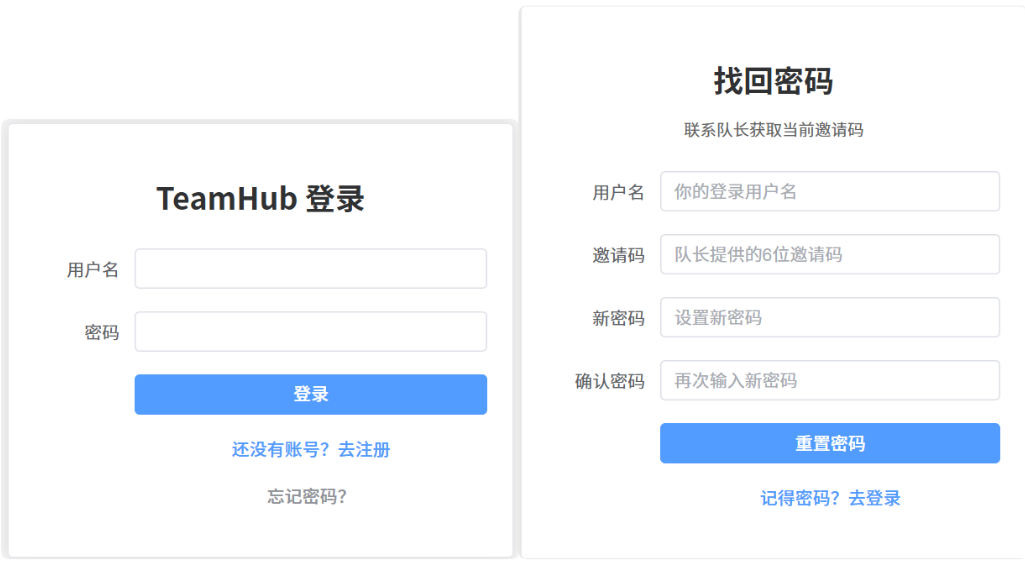
\includegraphics[width=0.85\textwidth]{截图/login.png}
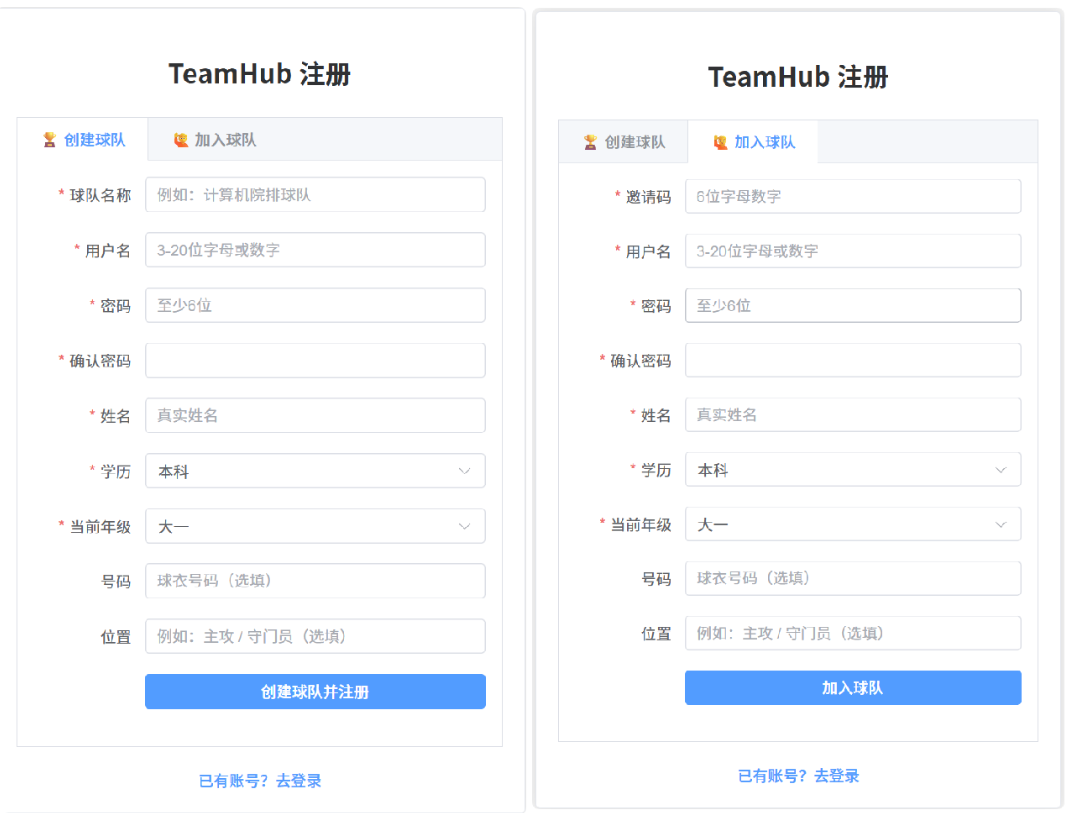
\includegraphics[width=0.85\textwidth]{截图/signup.png}
\caption{登录与注册界面}
\end{figure}
% 【图片位置】贴上登录页面截图

\textbf{首页仪表盘。}登录后进入主页，左侧展示个人信息卡片（头像、姓名、号码、年级）、最新自评和修改密码入口；中间展示本周训练列表（含报名状态标签）；右侧展示出勤率卡片、最近比赛和队友建议。队长额外看到待处理球队建议。

\begin{figure}[H]
\centering
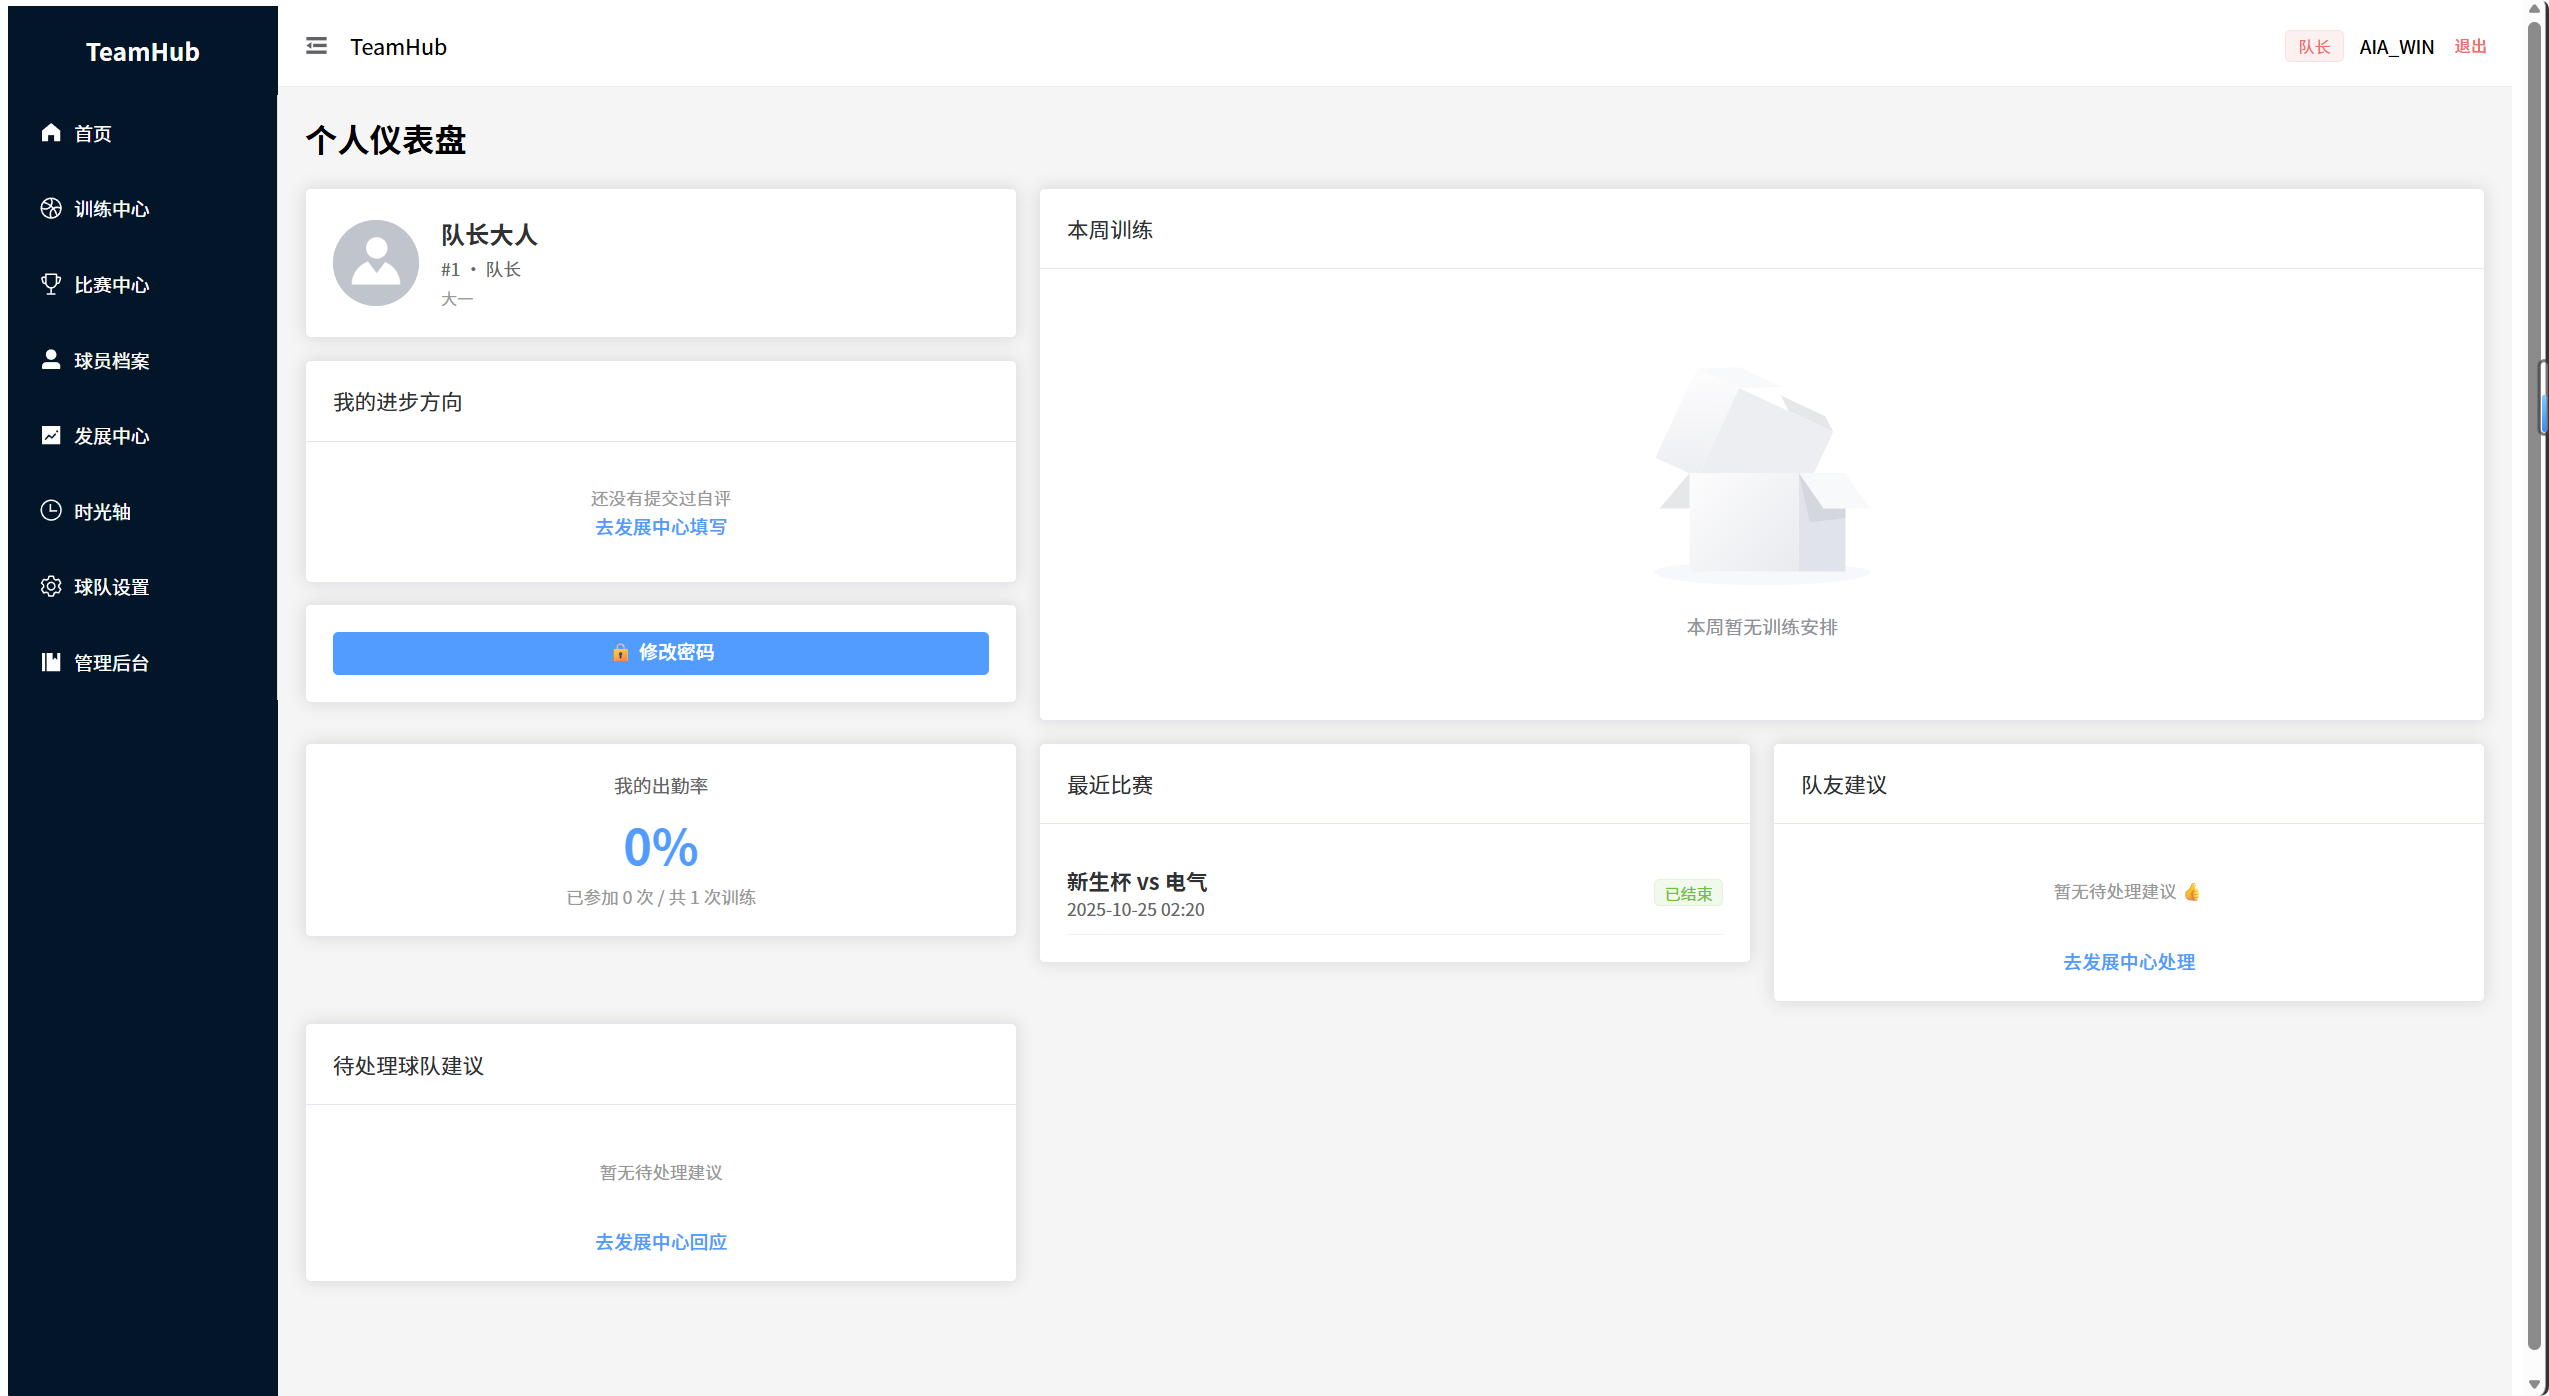
\includegraphics[width=0.85\textwidth]{截图/yibiaopan.png}
\caption{首页仪表盘原型}
\end{figure}
% 【图片位置】贴上首页仪表盘截图

\textbf{训练中心。}训练列表页按时间倒序展示所有训练，每条记录显示标题、地点、时间和当前用户的报名状态标签。队长可见"发布训练"按钮，点击后弹出el-dialog表单（标题、地点、时间选择器、内容文本域、视频链接）。点击训练卡片进入详情页，可查看训练计划、视频链接，并完成接龙报名（参加/请假/待定三个选项，请假需填理由）。

\begin{figure}[H]
\centering
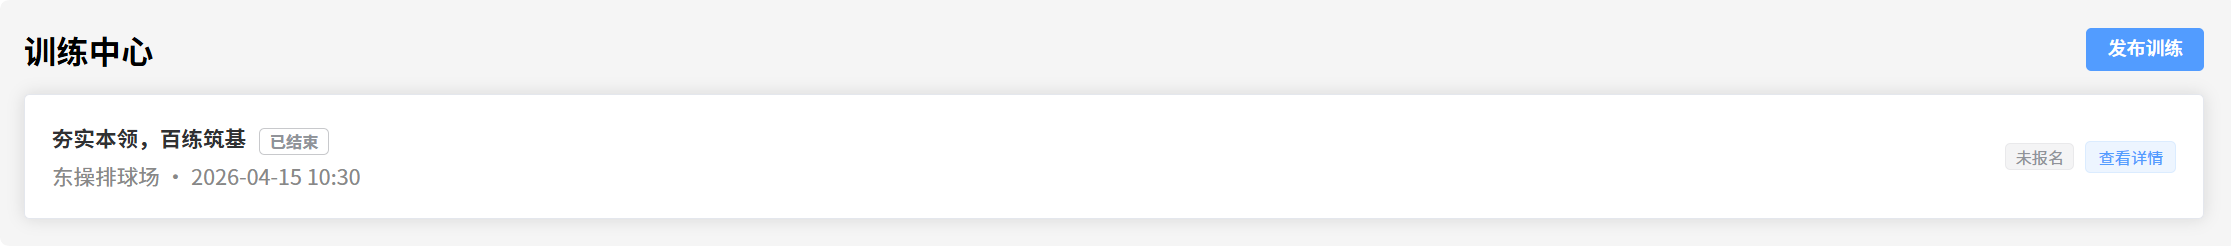
\includegraphics[width=0.85\textwidth]{截图/xunlian1.png}

\vspace{0.2cm}


\includegraphics[width=0.85\textwidth]{截图/xunlian2.png}

\vspace{0.2cm}

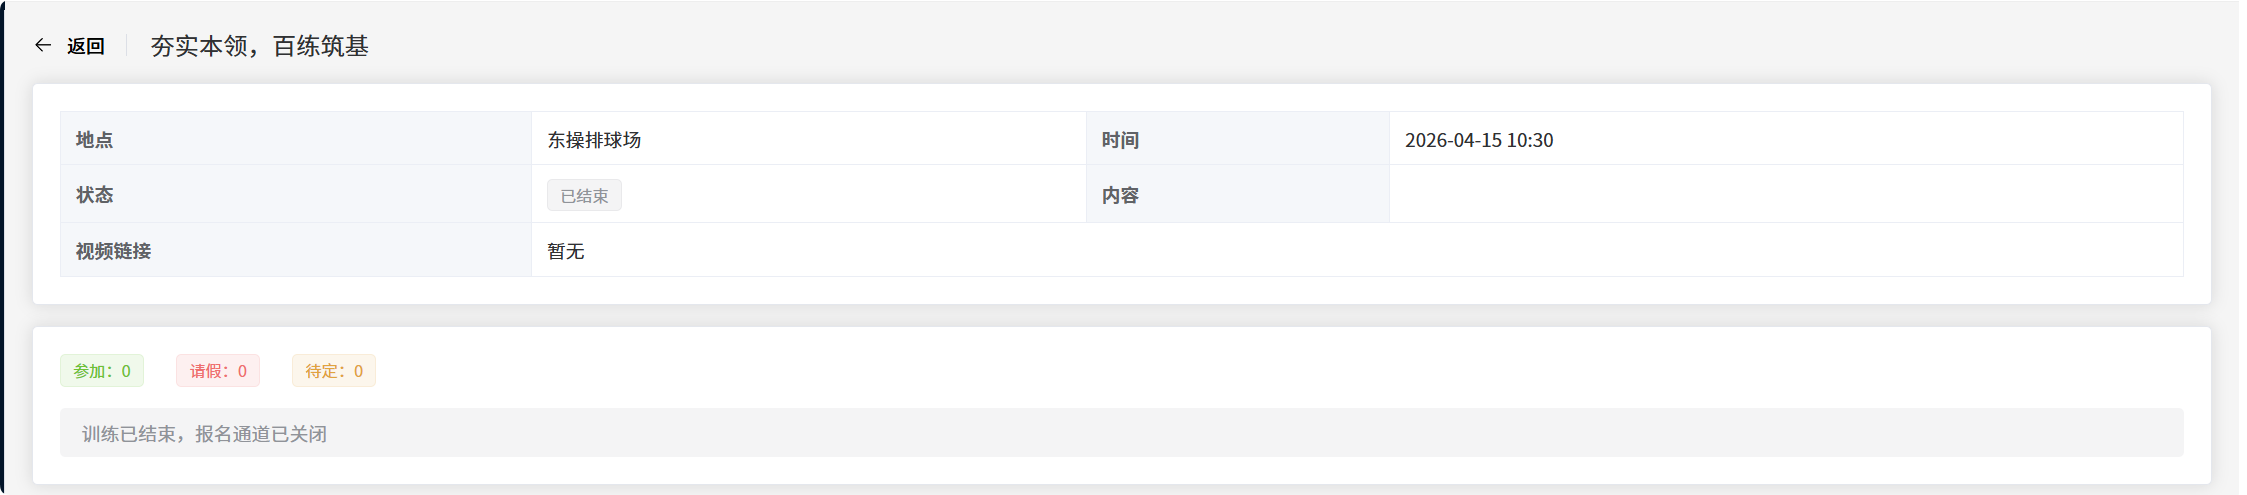
\includegraphics[width=0.85\textwidth]{截图/xunlian3.png}
\caption{训练列表与详情原型}
\end{figure}
% 【图片位置】贴上训练中心和训练详情页截图

\textbf{比赛中心。}比赛列表页顶部为el-radio-group赛事类型筛选栏（全部/训练赛/新生杯/华工杯/其他），下方为比赛卡片列表。点击进入比赛详情页，展示对手、时间、地点、比分（多局制时逐行显示局号和双方分数）、首发名单文本、战术总结和视频链接。队长可编辑比分（"先删后插"策略）、更新比赛状态（UPCOMING→ONGOING→FINISHED）、修改首发名单和视频链接。

\begin{figure}[H]
\centering
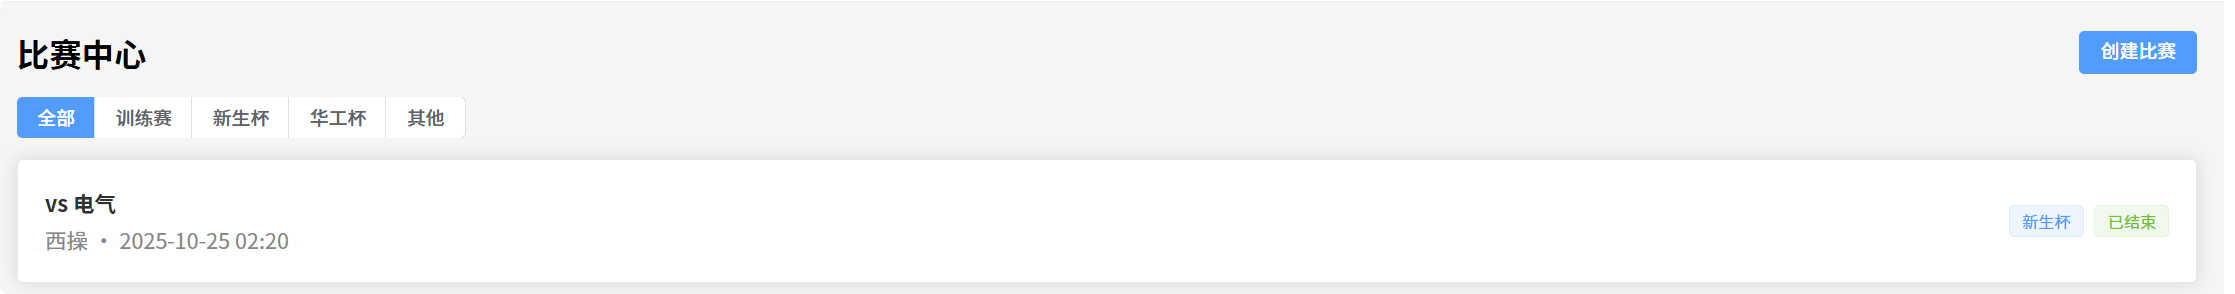
\includegraphics[width=0.85\textwidth]{截图/bisai1.png}

\vspace{0.2cm}

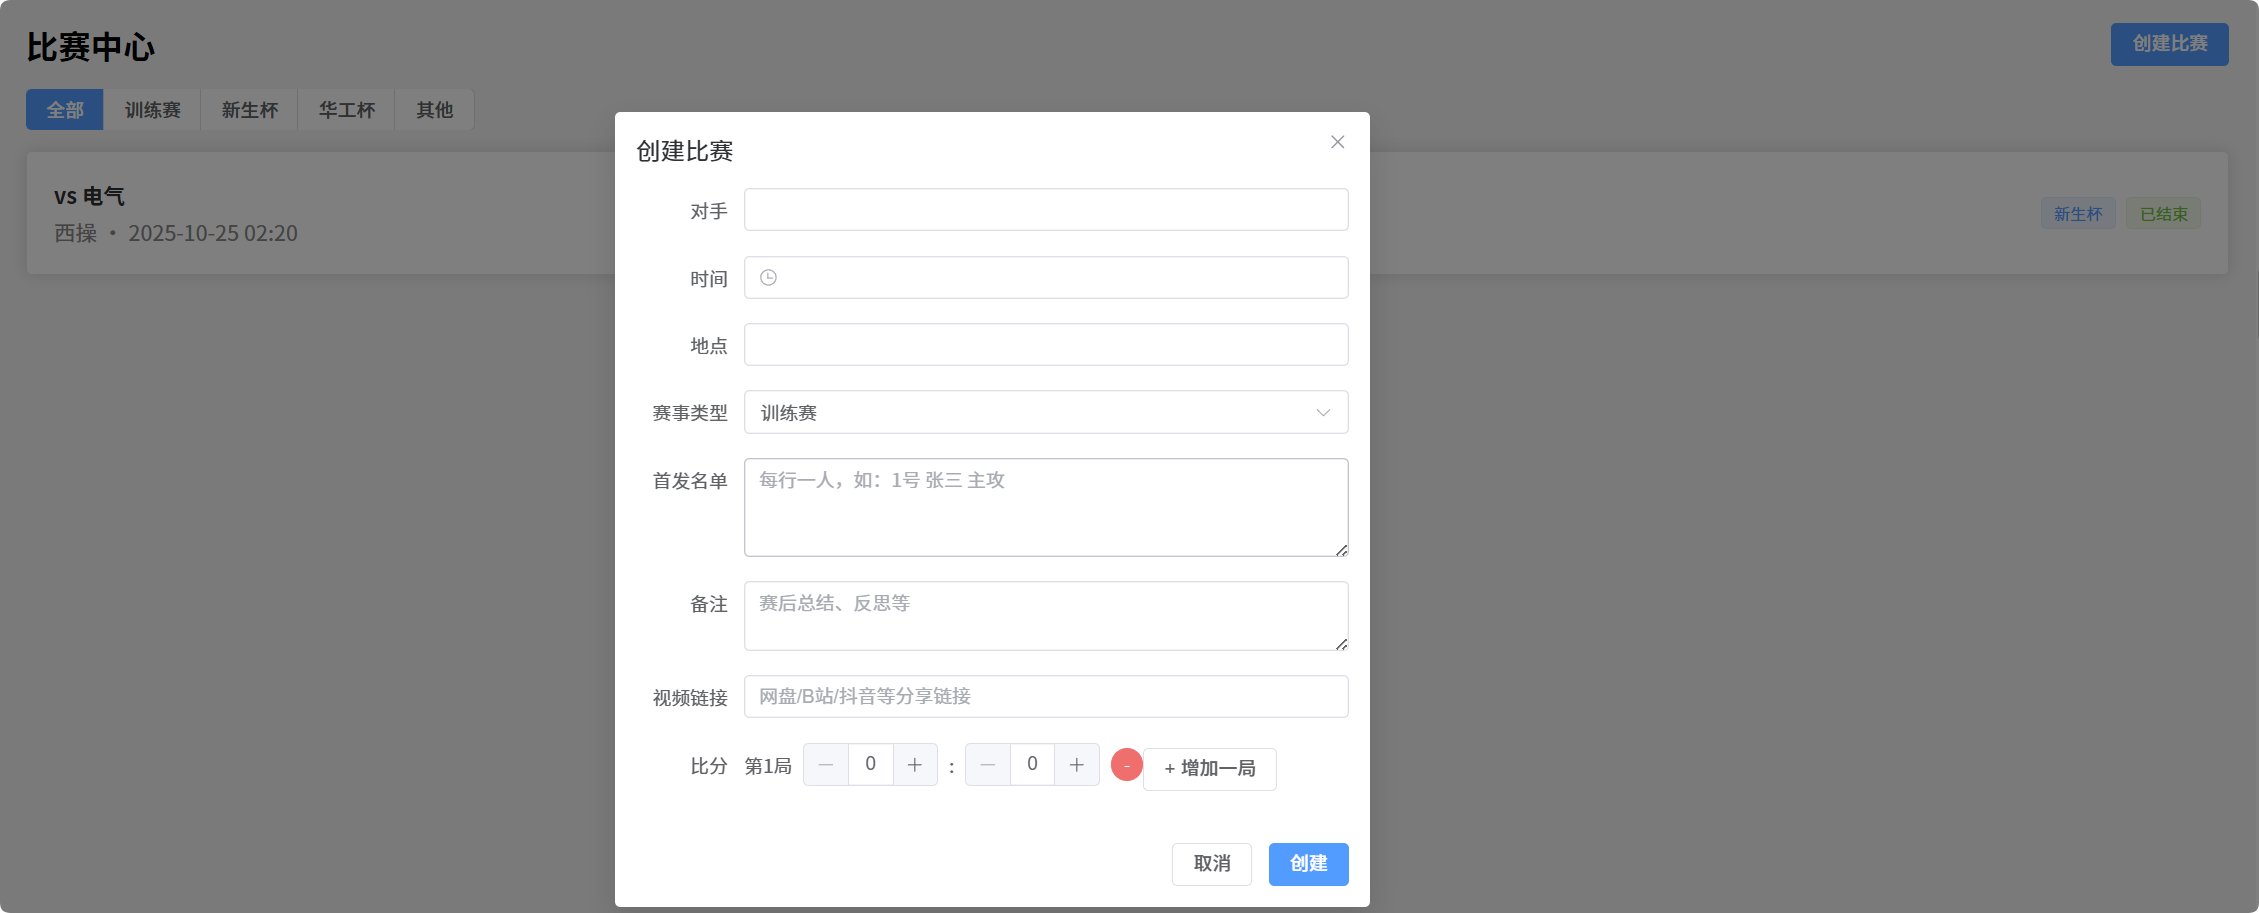
\includegraphics[width=0.85\textwidth]{截图/bisai2.png}

\vspace{0.2cm}

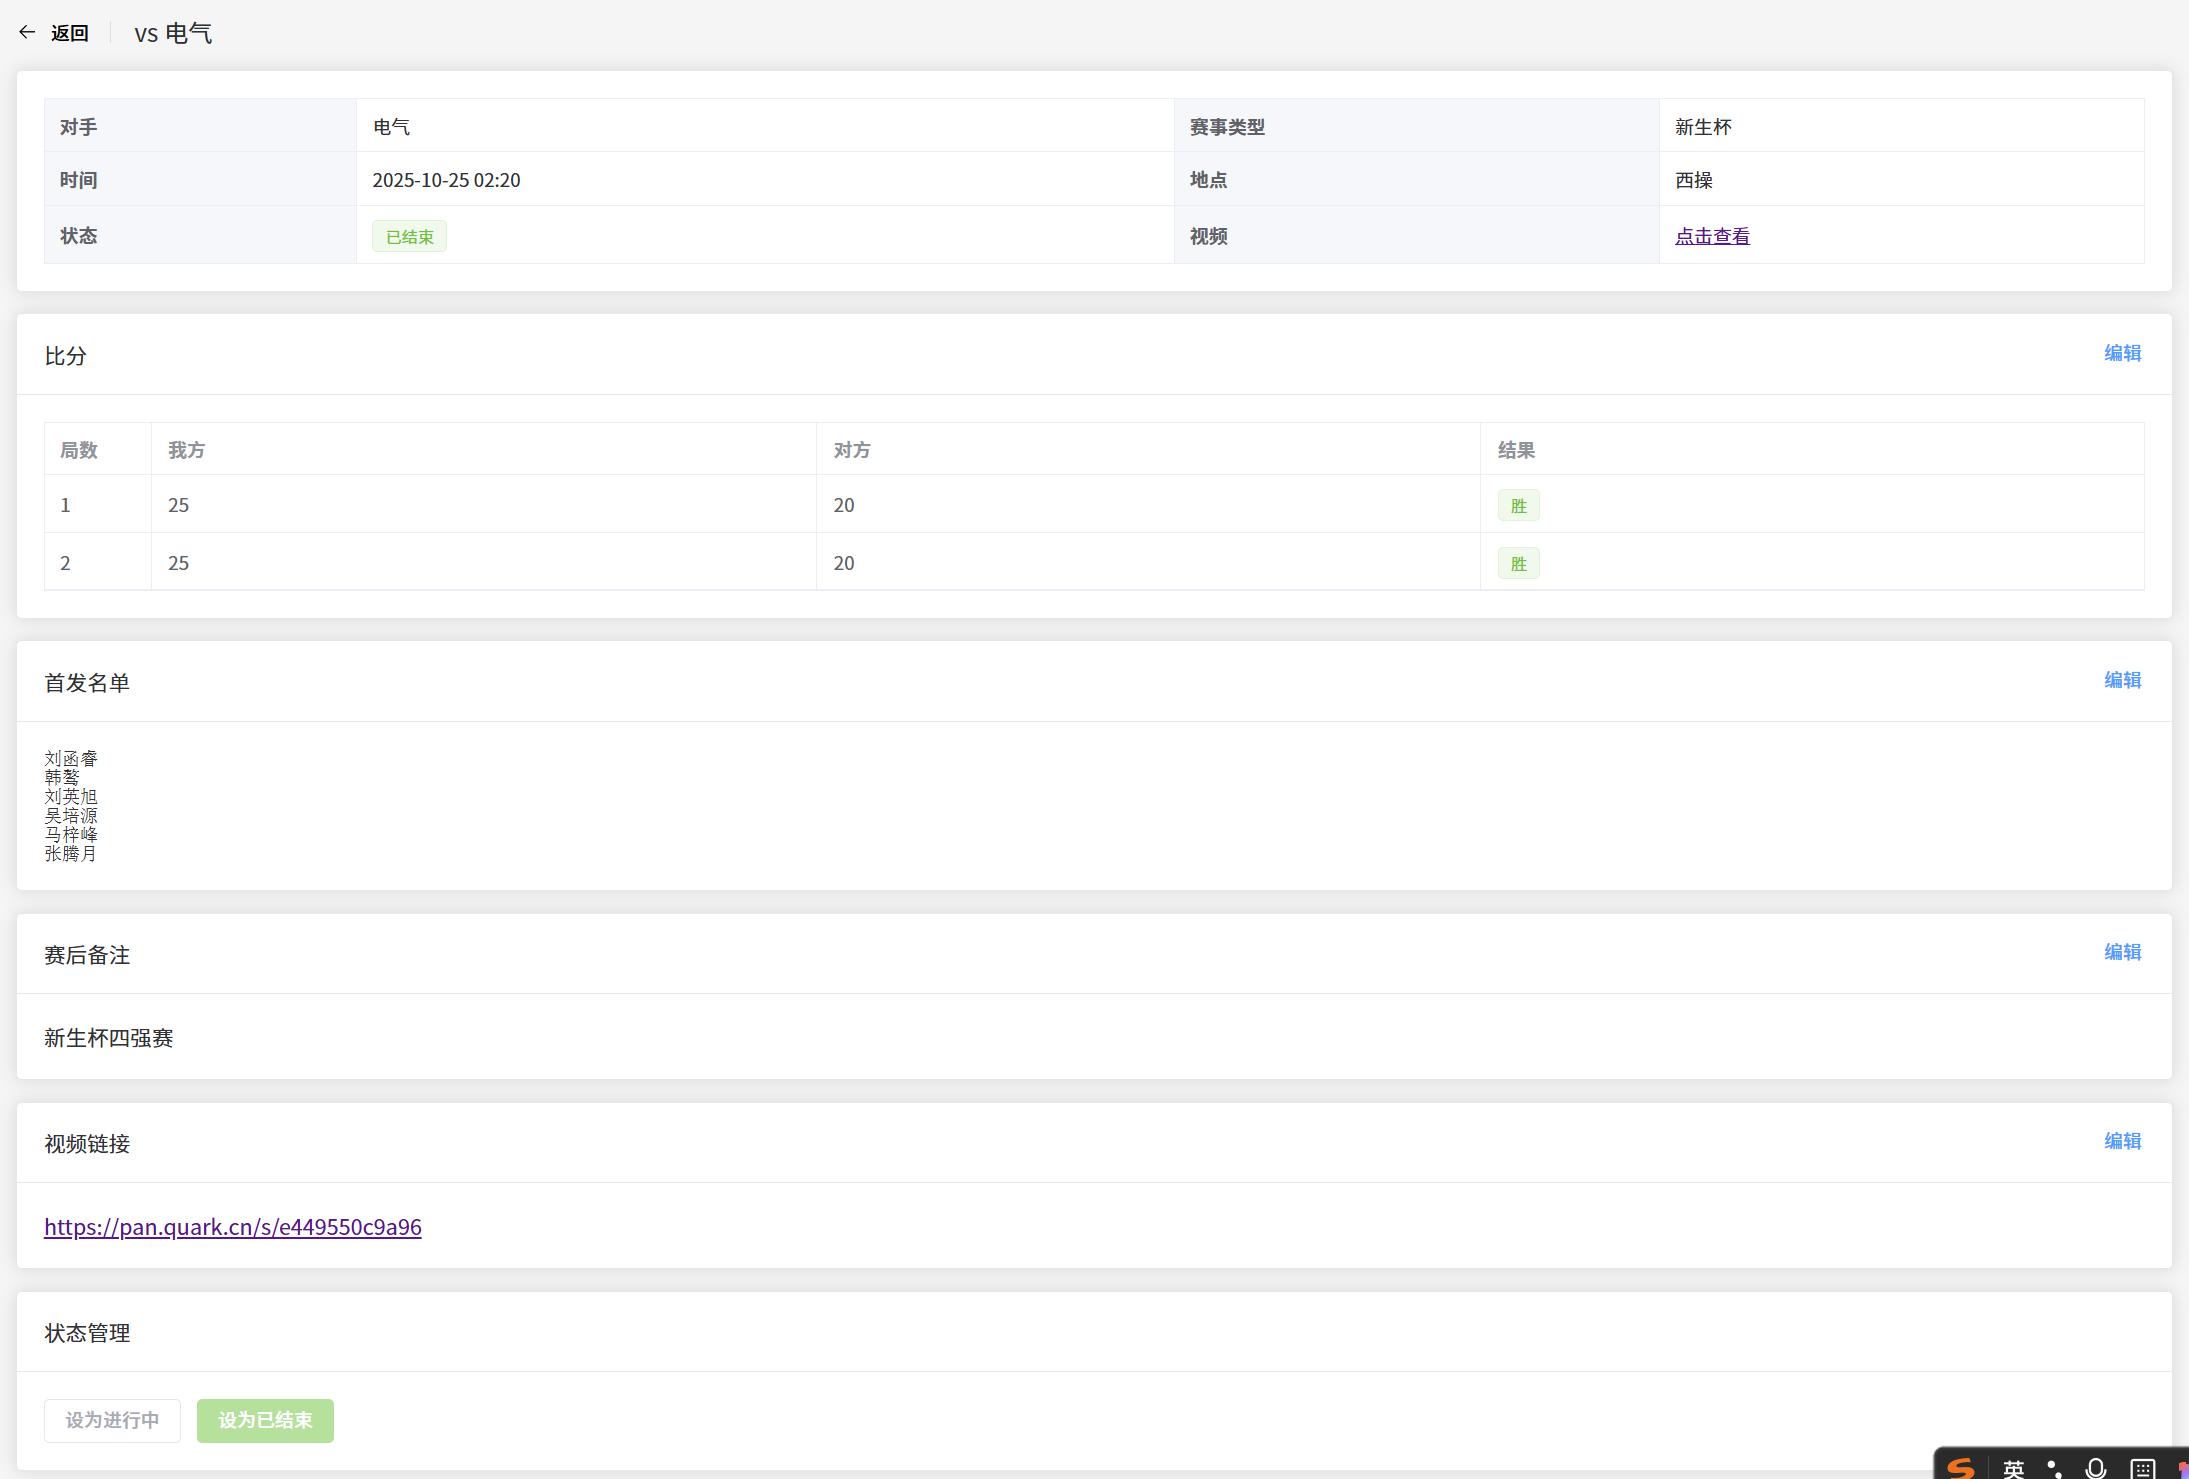
\includegraphics[width=0.85\textwidth]{截图/bisai3.png}

\caption{比赛列表与详情原型}
\end{figure}
% 【图片位置】贴上比赛中心和比赛详情页截图

\textbf{球员档案。}球员列表页分为"当打之年"和"功勋人物"两个el-tabs标签页，以el-row/el-col卡片网格展示球员头像、姓名、号码、位置和实时计算出的年级标签。点击卡片进入球员详情页查看完整信息。队长可编辑任一球员资料（含姓名），队员仅可编辑自己的部分信息（不含姓名）。队长可点击"毕业迁移"将球员从ACTIVE移至ALUMNI。

\begin{figure}[H]
\centering
% 上面两张上下排列
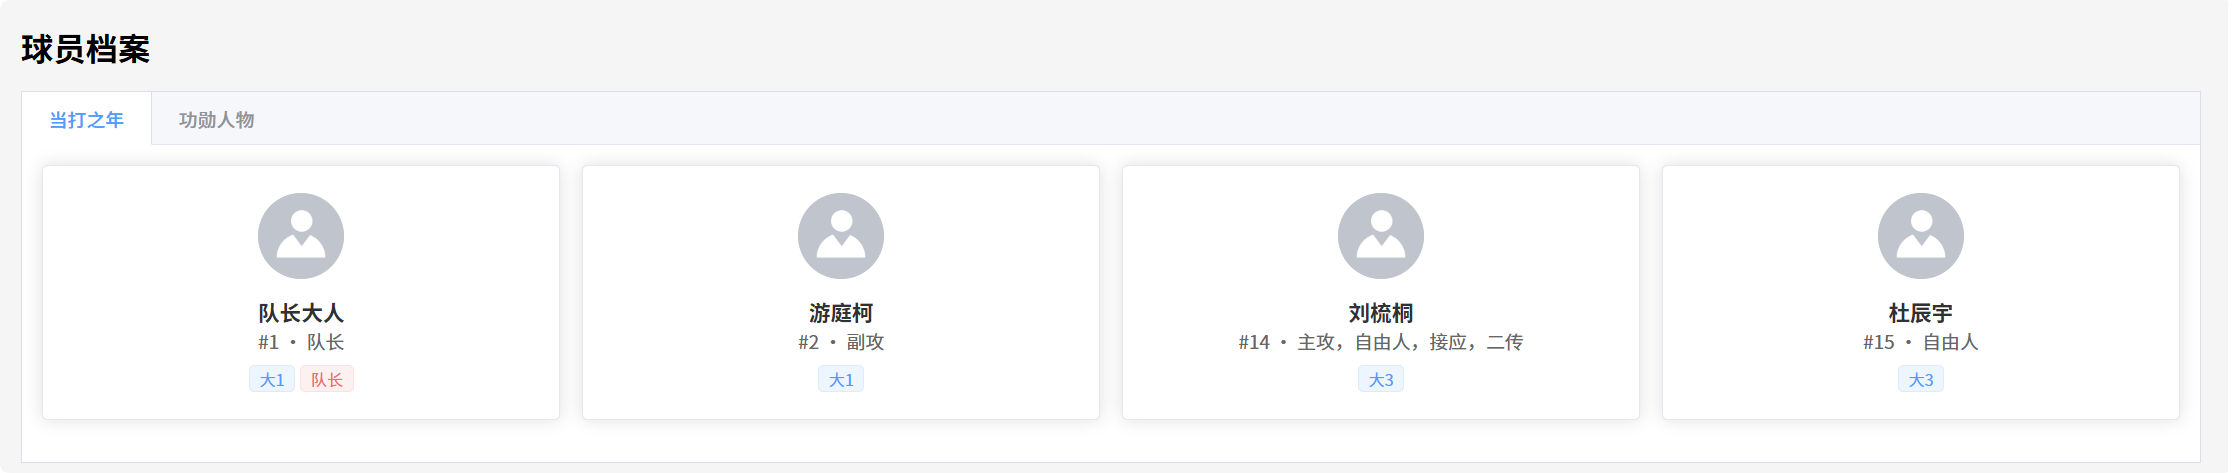
\includegraphics[width=0.85\textwidth]{截图/qiuyuan1.png}

\vspace{0.2cm}

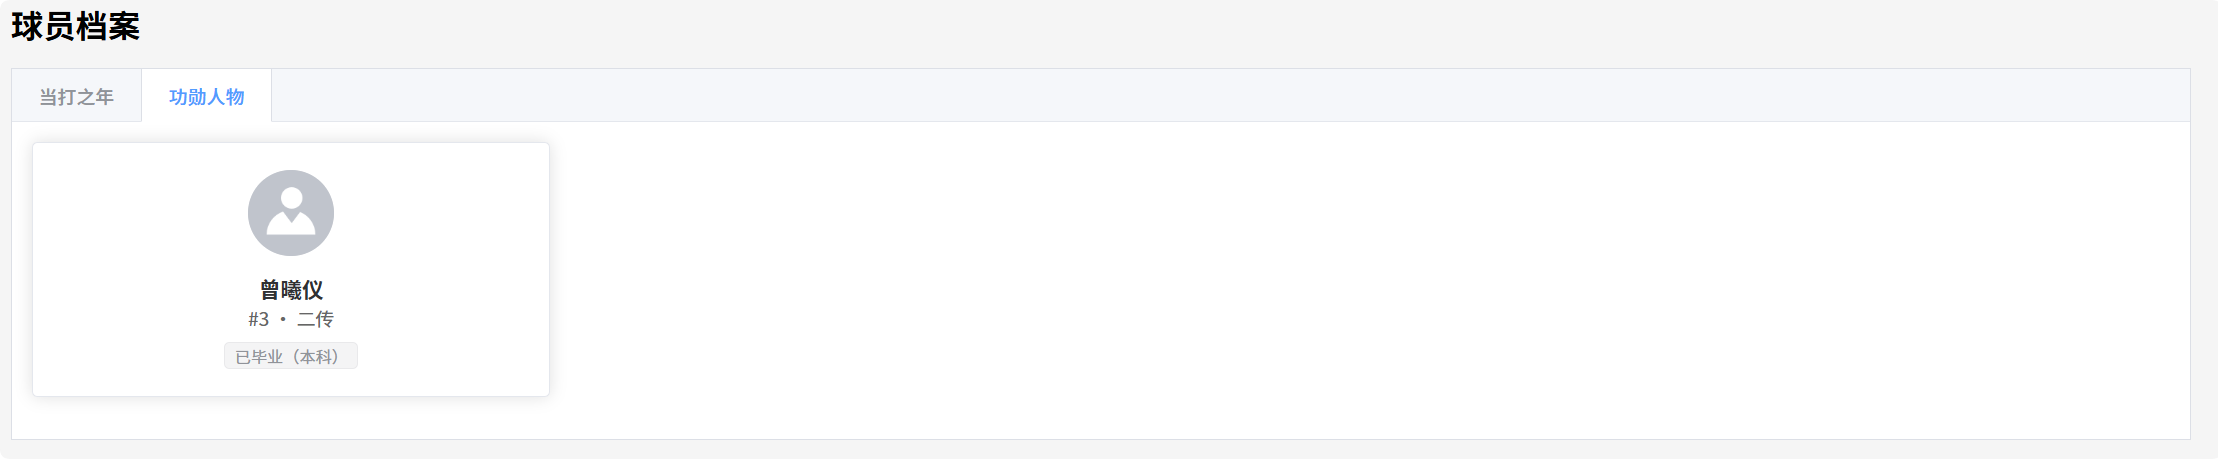
\includegraphics[width=0.85\textwidth]{截图/qiuyuan2.png}

\vspace{0.2cm}

% 下面两张左右并列
\begin{minipage}{0.42\textwidth}
    \centering
    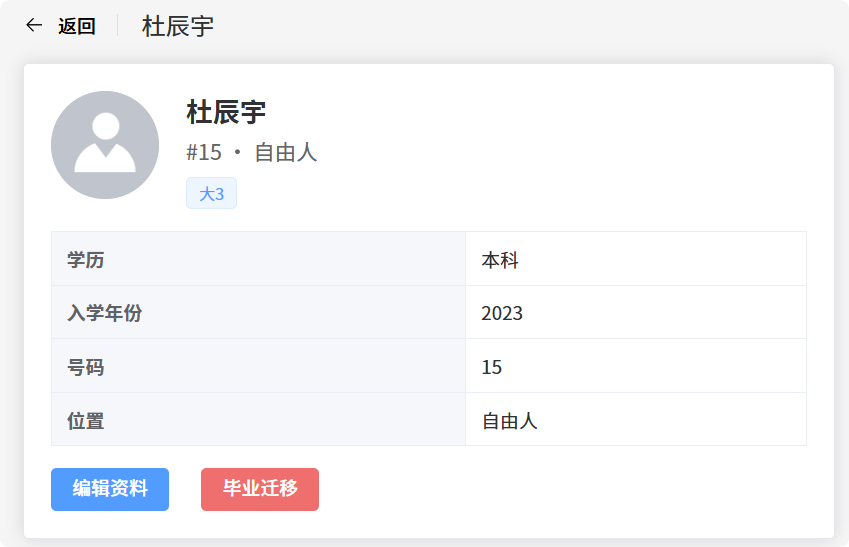
\includegraphics[width=\textwidth]{截图/qiuyuan3.png}
\end{minipage}

\hspace{1cm}

\begin{minipage}{0.42\textwidth}
    \centering
    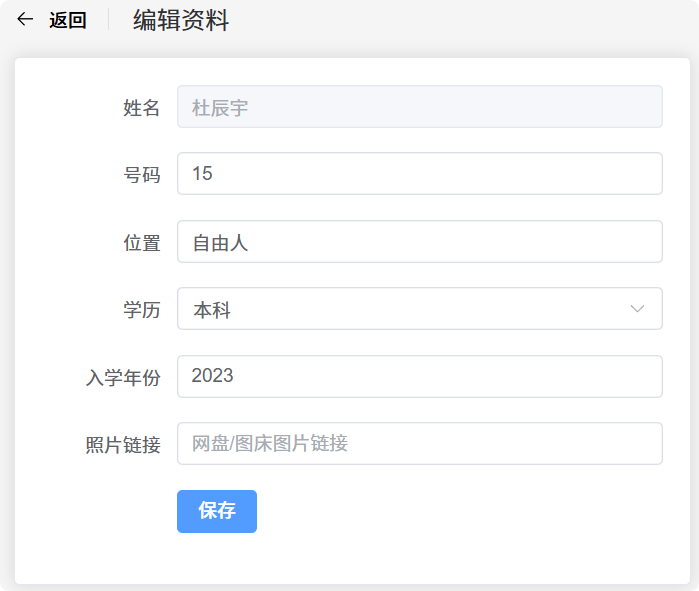
\includegraphics[width=\textwidth]{截图/qiuyuan4.png}
\end{minipage}

\caption{球员档案原型}
\end{figure}
% 【图片位置】贴上球员列表页截图

\textbf{发展中心。}分为三个el-tabs标签页。个人发展页包含自评表单（分类下拉、当前问题、改进目标、期望训练）、历史自评时间轴（el-timeline）和队友建议列表（每条建议显示分类标签、内容、点赞按钮、状态选择器、举报按钮）。全队自评页以卡片网格展示每个队员的最新自评摘要。球队建议页包含分类/状态筛选器、建议列表（含点赞、队长回应区），队长可在待处理建议上直接填写回应并选择采纳/暂不采纳/已落实。

{
\centering
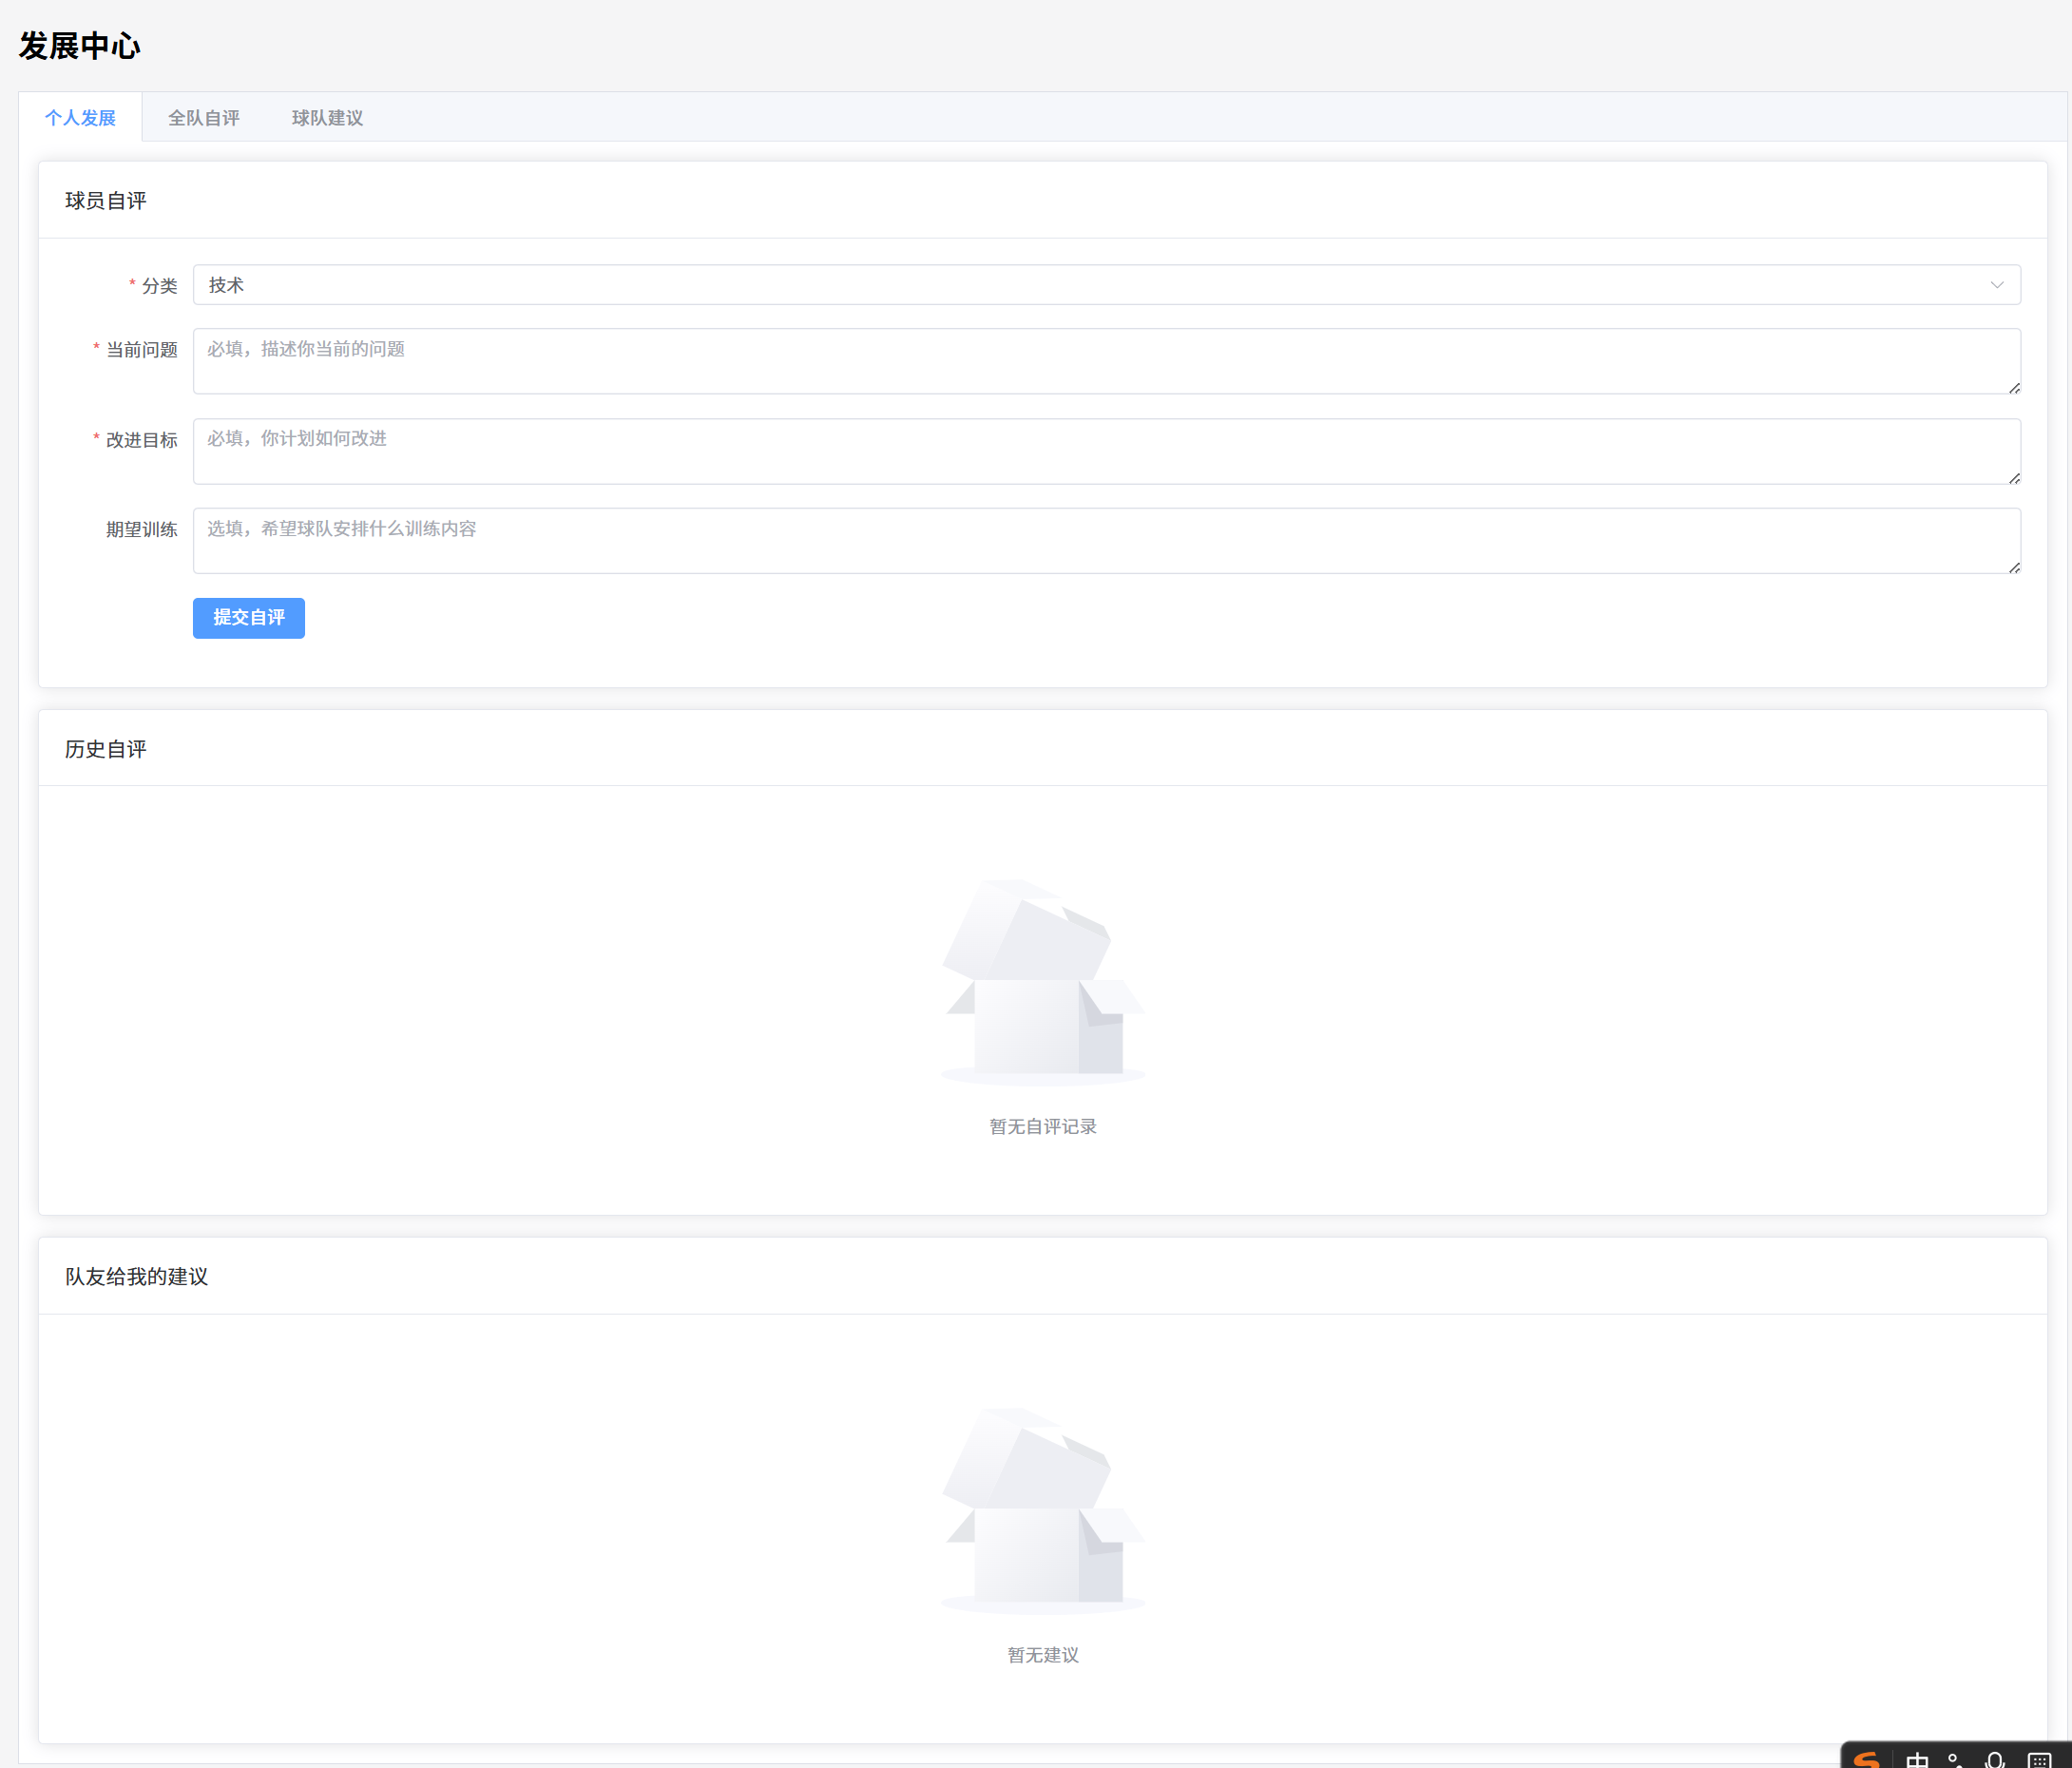
\includegraphics[width=0.85\textwidth]{截图/pinjia1.png}

\vspace{0.2cm}

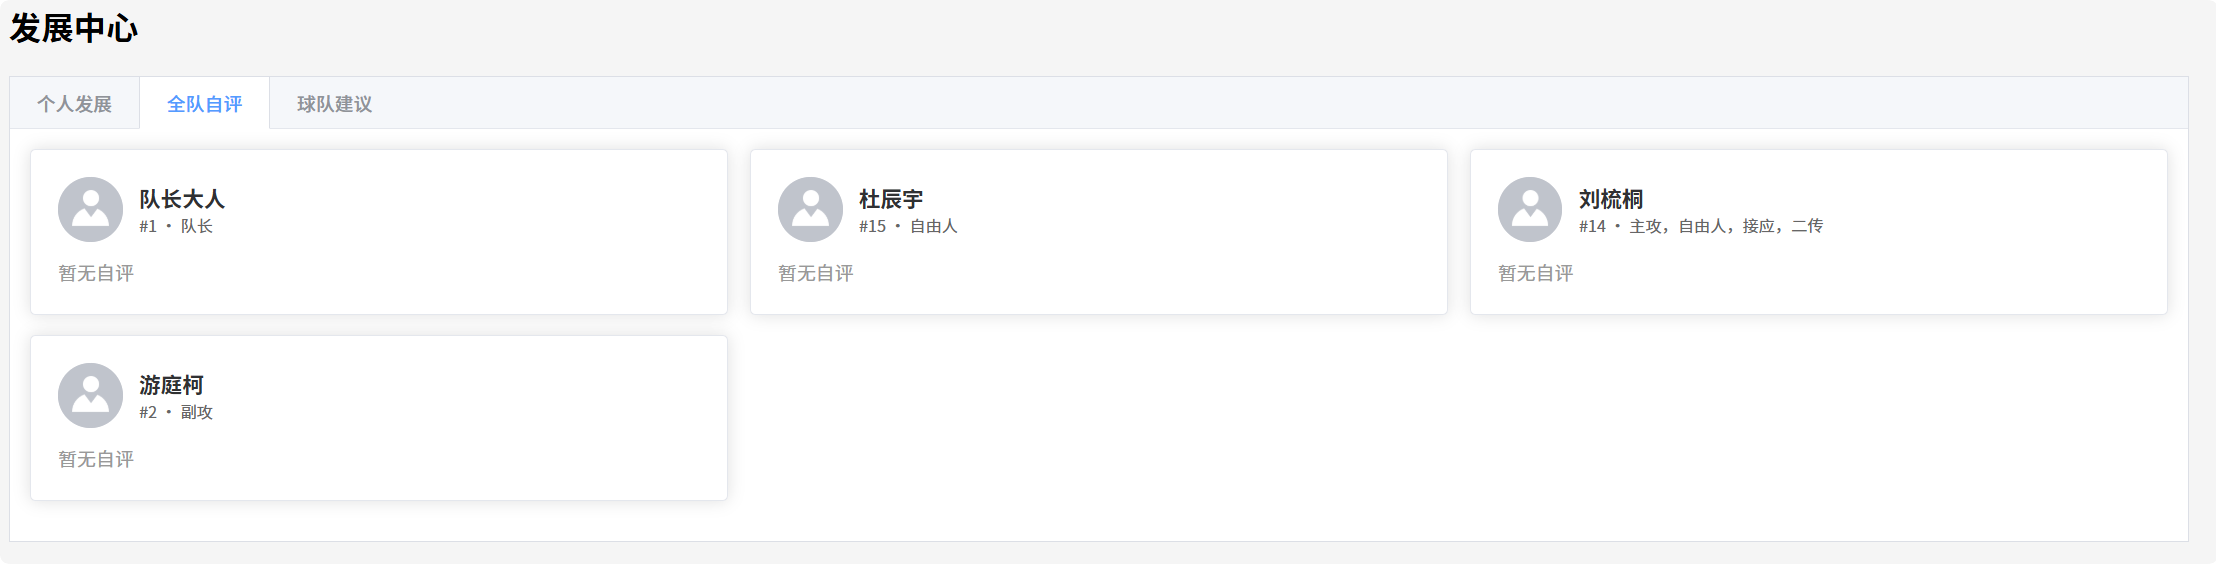
\includegraphics[width=0.85\textwidth]{截图/pinjia2.png}

\vspace{0.2cm}

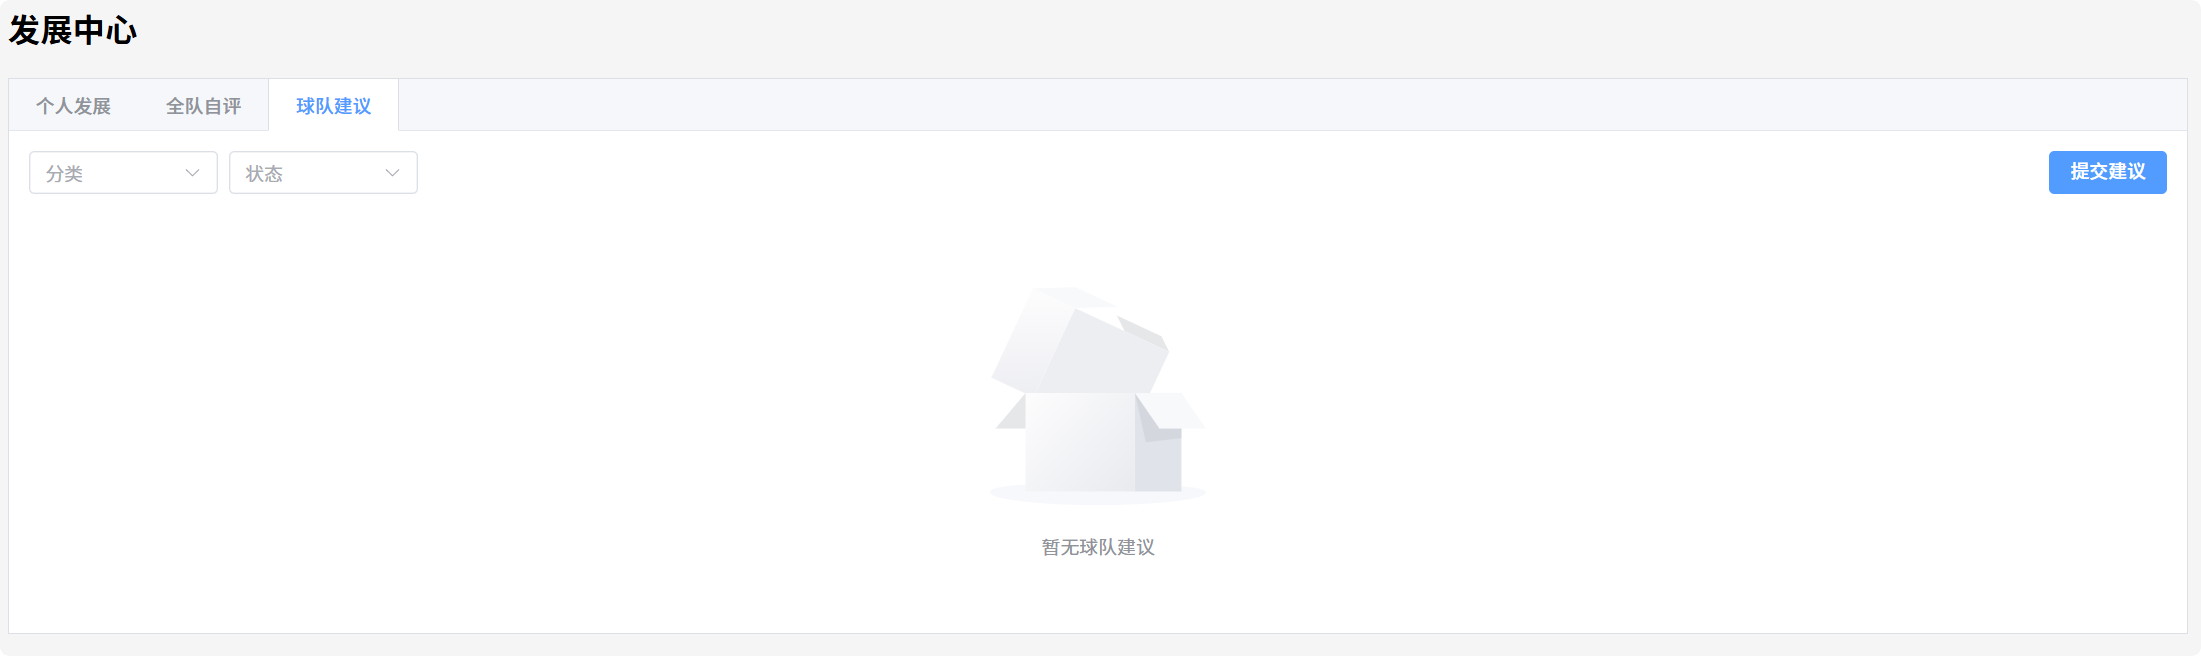
\includegraphics[width=0.85\textwidth]{截图/pinjia3.png}

\vspace{0.2cm}

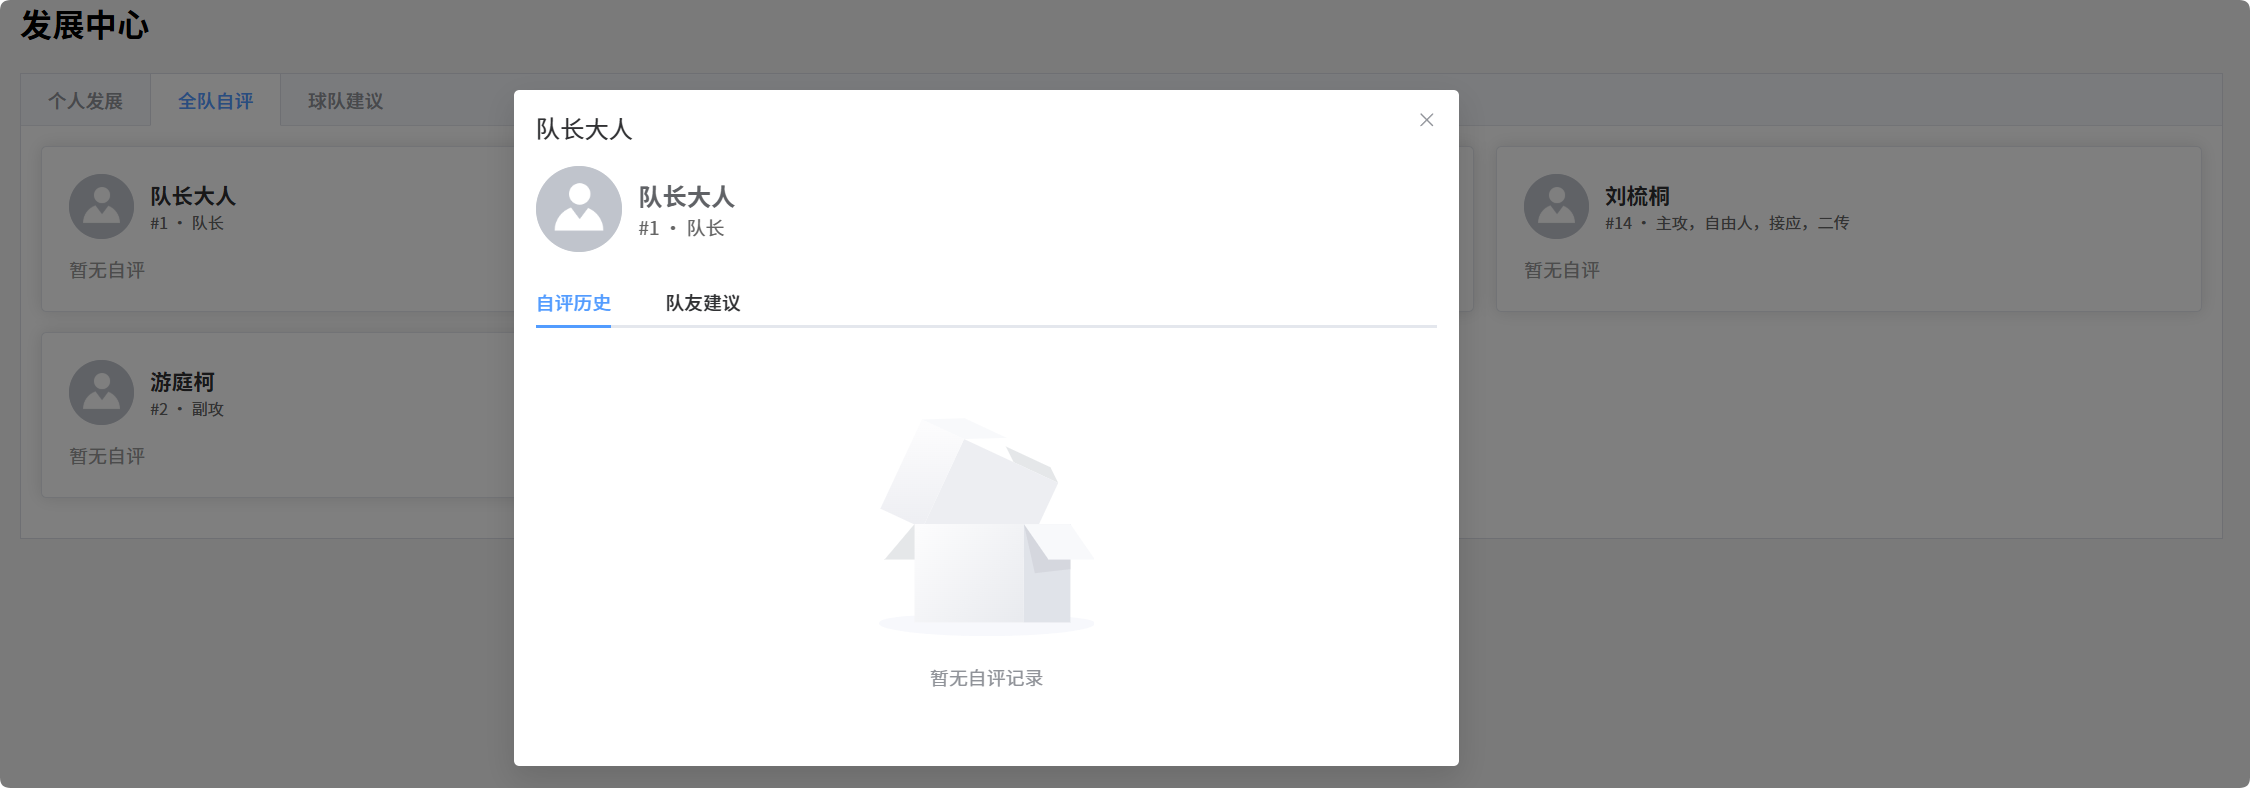
\includegraphics[width=0.85\textwidth]{截图/pinjia4.png}

\newpage


\includegraphics[width=0.85\textwidth]{截图/pinjia5.png}

\captionof{figure}{发展中心原型}
\par
}

% 【图片位置】贴上发展中心截图

\textbf{时光轴。}页面顶部为年份/月份选择器和重置按钮，下方为el-timeline时间河流。自动事件以灰色细线标记，人工事件以蓝色高亮显示。每条事件卡片可展开查看详情（标题、描述、图片、关联链接）。人工事件可编辑（仅作者和队长），发布时需选择关联类型（训练/比赛/球员）并填写对应ID。

\begin{figure}[H]
\centering
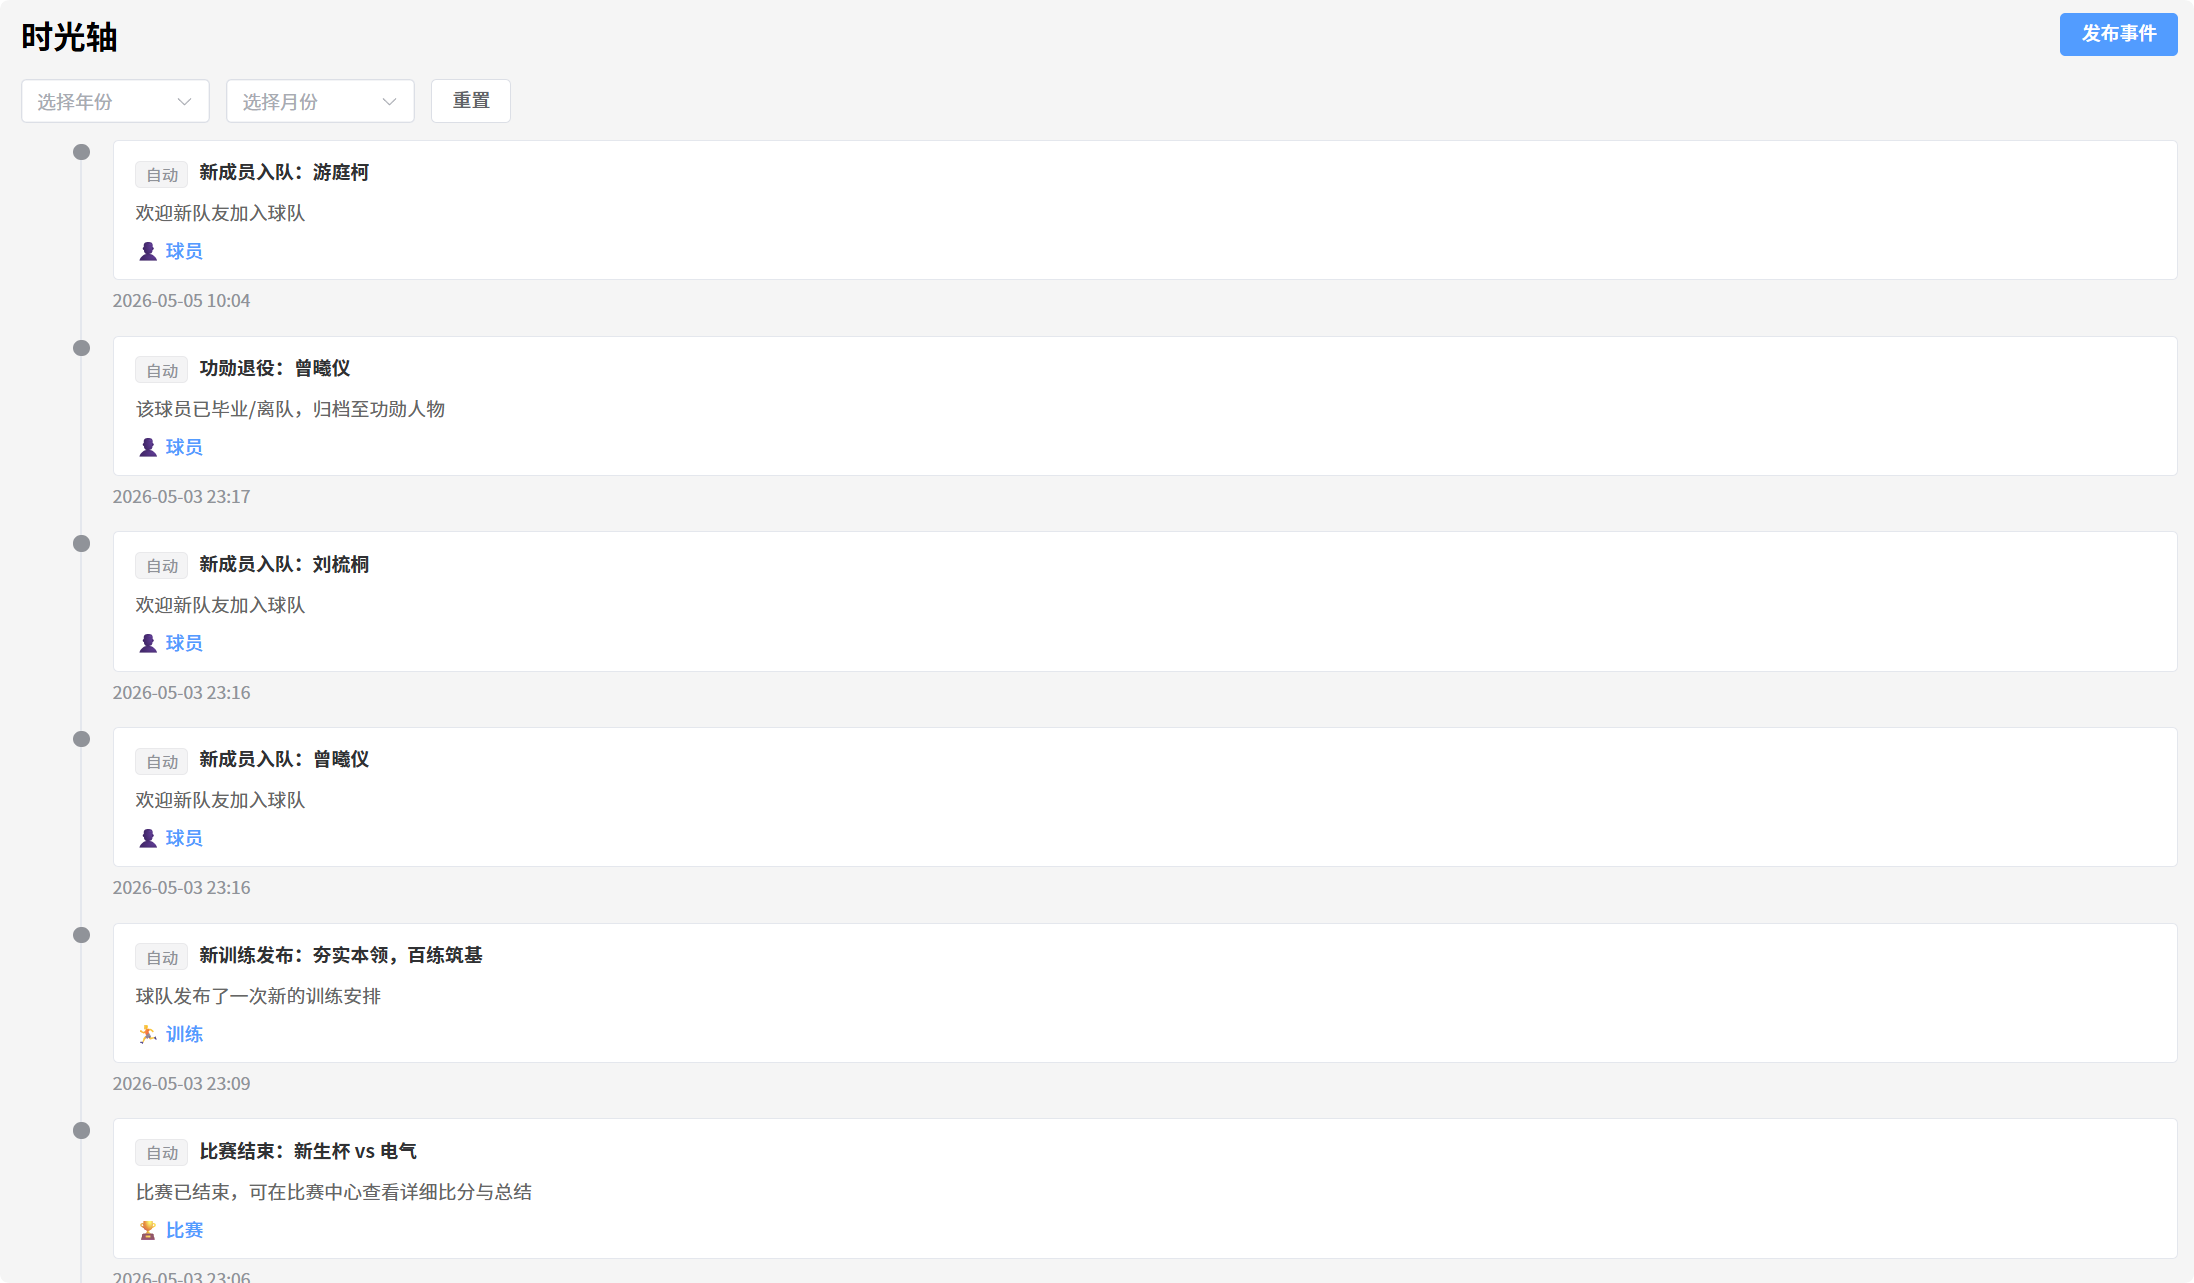
\includegraphics[width=0.85\textwidth]{截图/time1.png}

\vspace{0.2cm}

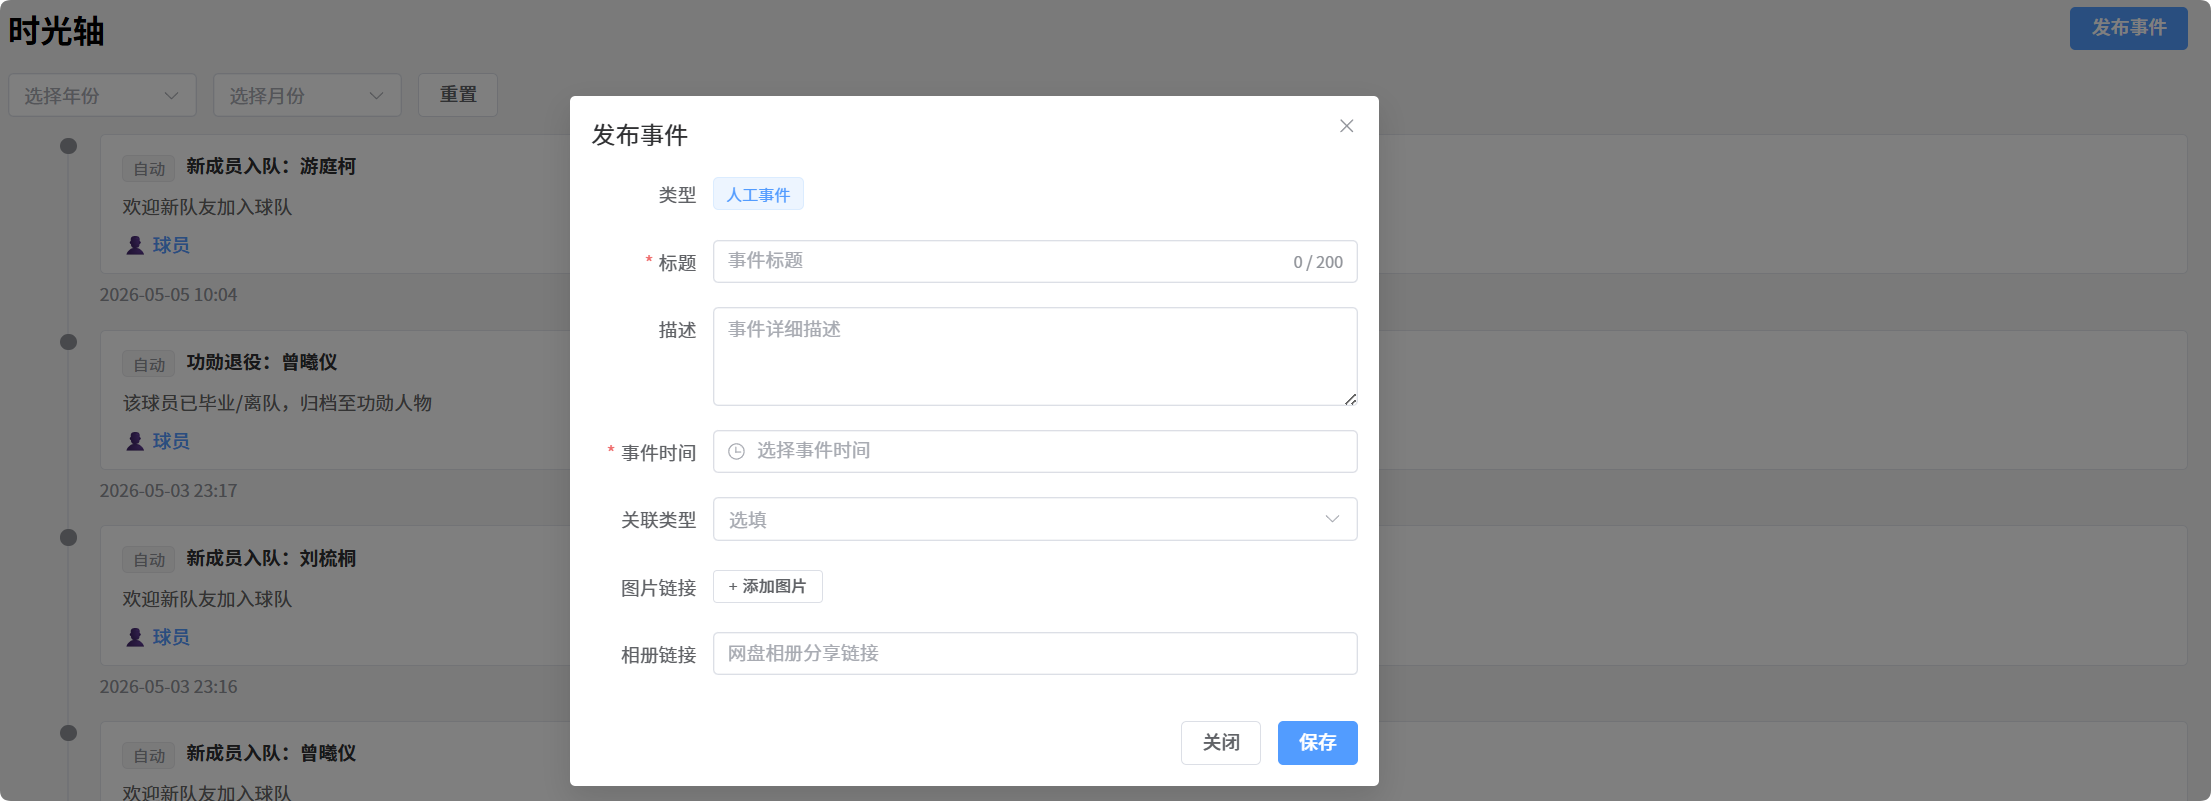
\includegraphics[width=0.85\textwidth]{截图/time2.png}
\caption{时光轴原型}
\end{figure}
% 【图片位置】贴上时光轴截图

\textbf{球队设置。}仅对队长开放，包含四大功能：邀请码管理（查看当前邀请码、有效期、剩余时间、重新生成）、修改队名、队长传承（选择队员后交接权限，原队长降级为MEMBER，新队长升级为CAPTAIN，双方需重新登录）、成员管理（表格展示所有成员，支持编辑姓名/学历/入学年份/号码/位置，或直接删除成员）、解散球队（仅当球队只剩队长一人时可执行，级联删除所有关联数据并清空登录态）。

\begin{figure}[H]
\centering

\caption{球队设置原型}
\end{figure}
{
\centering
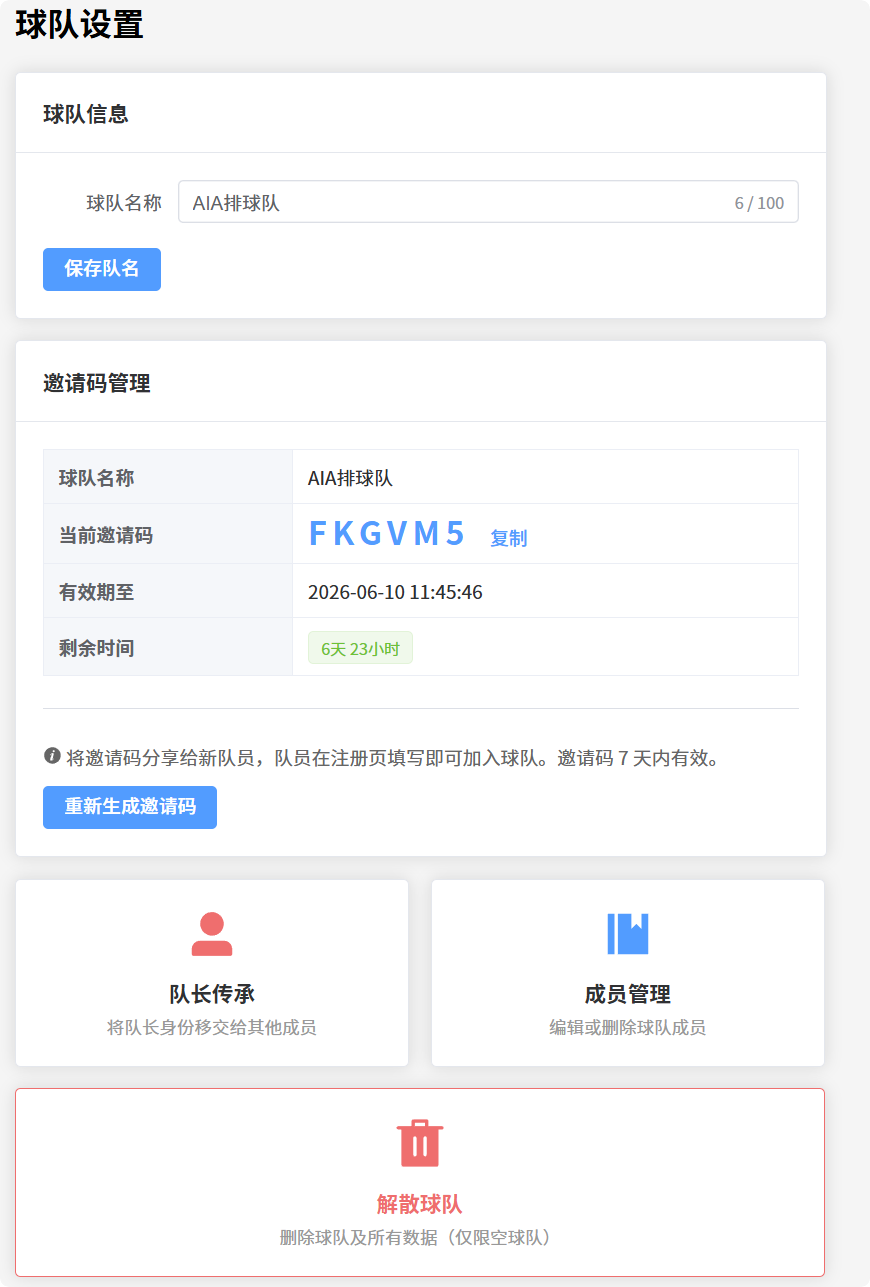
\includegraphics[width=0.60\textwidth]{截图/set1.png}

\vspace{0.2cm}

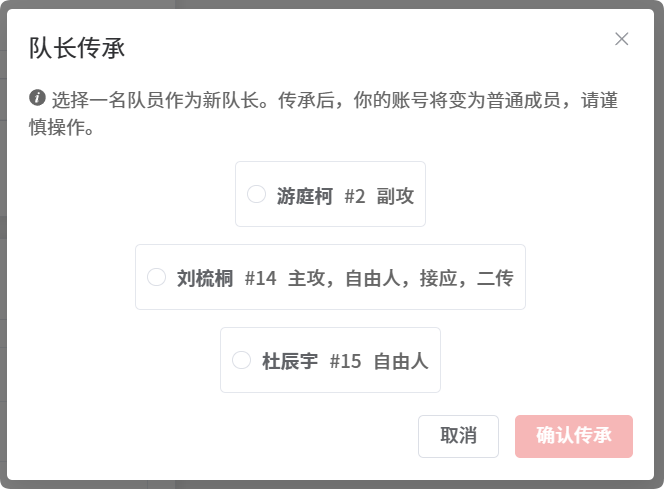
\includegraphics[width=0.50\textwidth]{截图/set2.png}

\newpage

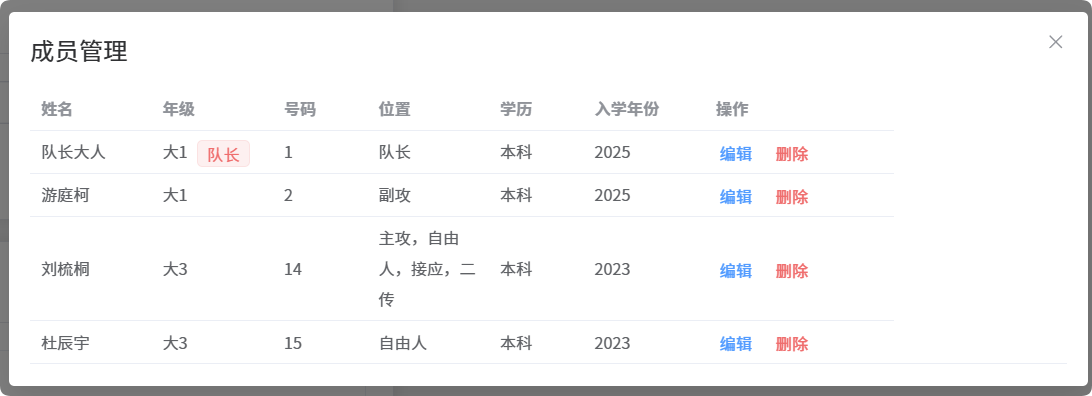
\includegraphics[width=0.55\textwidth]{截图/set3.png}

\captionof{figure}{发展中心原型}
\par
}
% 【图片位置】贴上球队设置页面截图

\textbf{管理后台。}仅对队长开放，包含被举报建议审核（查看被举报的建议，选择忽略或删除）。

\begin{figure}[H]
\centering
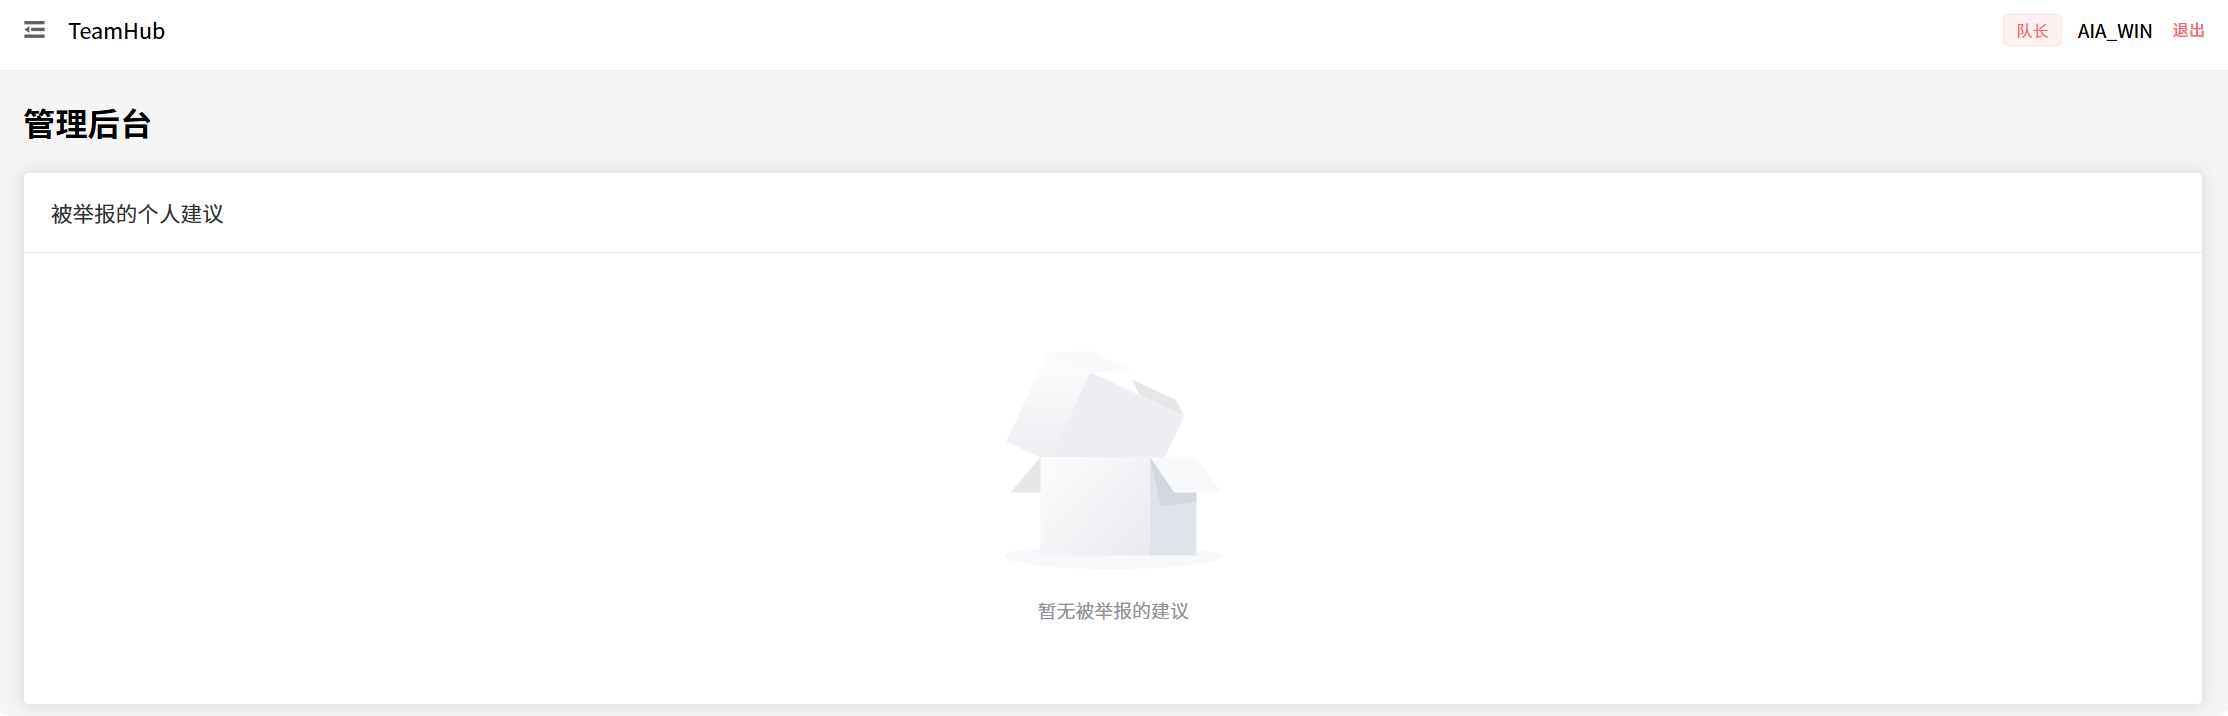
\includegraphics[width=0.85\textwidth]{截图/houtai1.png}
\caption{管理后台原型}
\end{figure}

% ==============================
%  第3章 概要设计和详细设计
% ==============================
\newpage
\section{概要设计和详细设计}

\subsection{系统整体结构}

\subsubsection{前后端分层架构}

系统采用前后端分离的B/S架构。前端为Vue 3单页应用，通过Axios发送HTTP请求，经Nginx代理转发到后端Tomcat。后端采用标准的分层架构。

前端层：Vue 3 + TypeScript + Vite 8.0.8构建，Element Plus 2.13.7负责UI，Vue Router 5.0.4管理路由（带导航守卫检查Token），Axios 1.15.2封装了请求拦截器（注入Bearer Token）和响应拦截器（401跳登录、403提示无权操作、400交给业务代码处理）。Layout.vue实现了桌面端el-aside侧边栏（支持折叠）和移动端el-drawer抽屉的响应式切换（通过window.innerWidth < 768判断）。

后端层：Controller层接收HTTP请求、校验参数并委托Service处理。Service层封装业务逻辑，使用MyBatis-Plus的QueryWrapper构建动态SQL，调用Mapper层操作数据库。配置层包括SecurityConfig（无状态会话、CORS白名单、公开接口放行）、JwtUtil（HS256签名、7天过期）、JwtAuthenticationFilter（从Authorization头解析Token、校验用户存在性后设置SecurityContext）、GlobalExceptionHandler（RuntimeException→400、AccessDeniedException→403、AuthenticationException→401）。

数据层：MySQL 8 + InnoDB引擎，13张业务表，字符集UTF-8MB4。MyBatis-Plus配置驼峰转下划线，开发环境输出SQL日志。

具体技术版本为：Spring Boot 3.5.14、Java 17、MyBatis-Plus 3.5.12、Vue 3.5.32、Vite 8.0.8、Element Plus 2.13.7、MySQL 8.0。

\subsubsection{UML类图}

本系统最重要的部分为用户认证和训练比赛事务。用户认证部分的UML类图如图\ref{fig:class-auth}所示。

\begin{figure}[H]
\centering
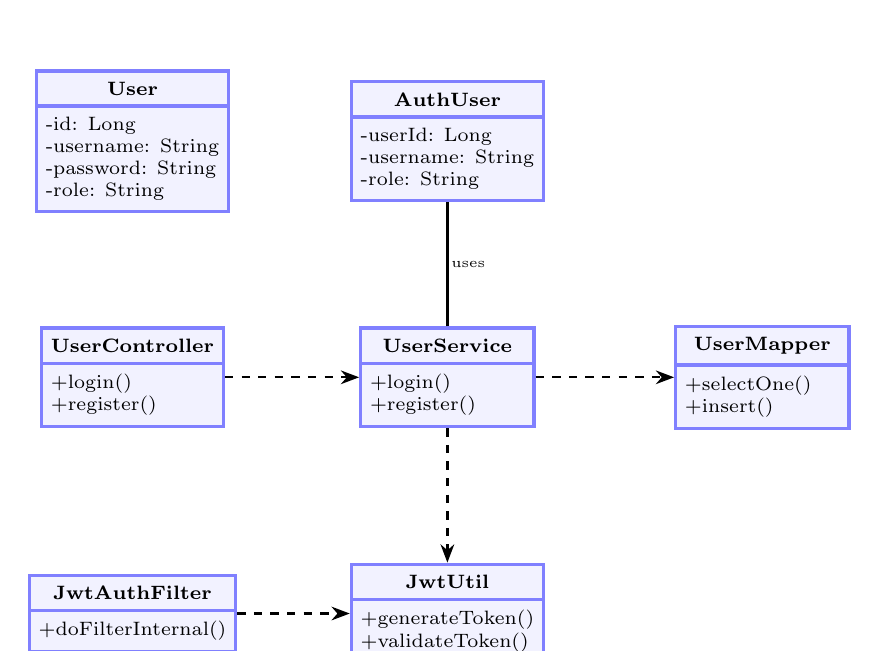
\begin{tikzpicture}[
    class/.style={rectangle split, rectangle split parts=2, draw=blue!50, fill=blue!5, very thick, minimum width=2.2cm, align=left, font=\scriptsize, rectangle split part align={center, left}},
    dep/.style={-{Stealth}, thick, dashed},
    assoc/.style={thick},
    label/.style={font=\tiny, fill=white, inner sep=1pt}]
\node[class] (user) at (0,0) {\textbf{User}\nodepart{second} -id: Long\\-username: String\\-password: String\\-role: String};
\node[class] (auth) at (4,0) {\textbf{AuthUser}\nodepart{second} -userId: Long\\-username: String\\-role: String};
\node[class] (ctrl) at (0,-3) {\textbf{UserController}\nodepart{second} +login()\\+register()};
\node[class] (svc) at (4,-3) {\textbf{UserService}\nodepart{second} +login()\\+register()};
\node[class] (mapper) at (8,-3) {\textbf{UserMapper}\nodepart{second} +selectOne()\\+insert()};
\node[class] (jwt) at (4,-6) {\textbf{JwtUtil}\nodepart{second} +generateToken()\\+validateToken()};
\node[class] (filter) at (0,-6) {\textbf{JwtAuthFilter}\nodepart{second} +doFilterInternal()};
\draw[dep] (ctrl) -- (svc);
\draw[dep] (svc) -- (mapper);
\draw[dep] (svc) -- (jwt);
\draw[dep] (filter) -- (jwt);
\draw[assoc] (svc) -- node[label, right] {uses} (auth);
\end{tikzpicture}
\caption{用户认证类图}
\label{fig:class-auth}
\end{figure}
% 【图片位置】贴上用户认证UML类图

训练比赛事务部分的UML类图如图\ref{fig:class-business}所示。

\begin{figure}[H]
\centering
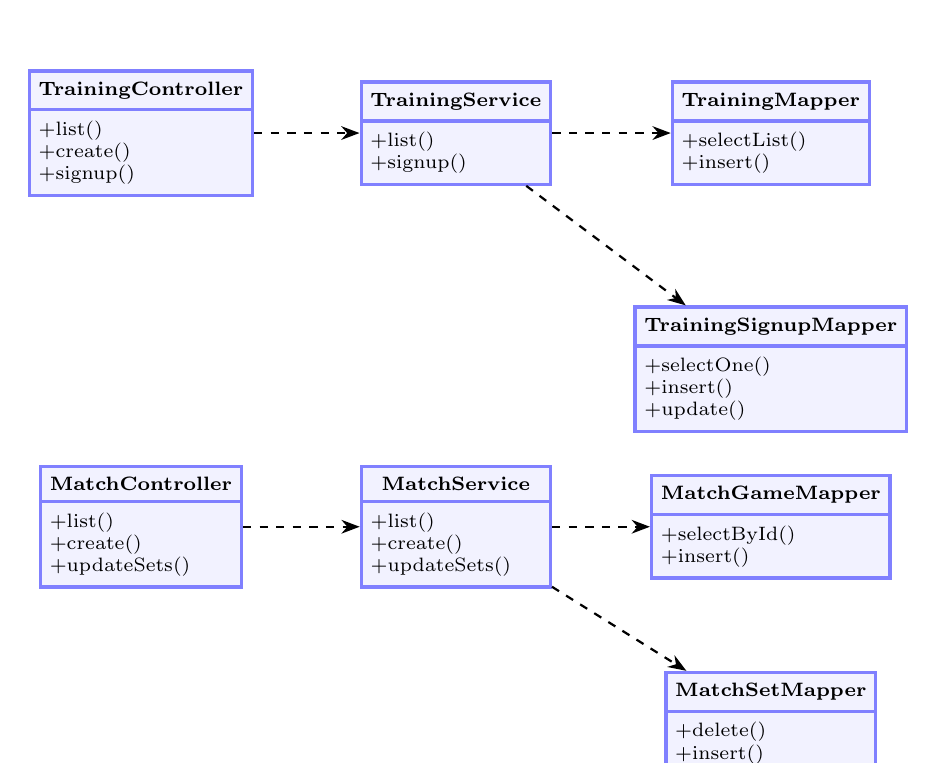
\begin{tikzpicture}[
    class/.style={rectangle split, rectangle split parts=2, draw=blue!50, fill=blue!5, very thick, minimum width=2.4cm, align=left, font=\scriptsize, rectangle split part align={center, left}},
    dep/.style={-{Stealth}, thick, dashed},
    font=\scriptsize]
\node[class] (tc) at (0,0) {\textbf{TrainingController}\nodepart{second} +list()\\+create()\\+signup()};
\node[class] (ts) at (4,0) {\textbf{TrainingService}\nodepart{second} +list()\\+signup()};
\node[class] (tm) at (8,0) {\textbf{TrainingMapper}\nodepart{second} +selectList()\\+insert()};
\node[class] (tsm) at (8,-3) {\textbf{TrainingSignupMapper}\nodepart{second} +selectOne()\\+insert()\\+update()};
\node[class] (mc) at (0,-5) {\textbf{MatchController}\nodepart{second} +list()\\+create()\\+updateSets()};
\node[class] (ms) at (4,-5) {\textbf{MatchService}\nodepart{second} +list()\\+create()\\+updateSets()};
\node[class] (mgm) at (8,-5) {\textbf{MatchGameMapper}\nodepart{second} +selectById()\\+insert()};
\node[class] (msm) at (8,-7.5) {\textbf{MatchSetMapper}\nodepart{second} +delete()\\+insert()};
\draw[dep] (tc) -- (ts);
\draw[dep] (ts) -- (tm);
\draw[dep] (ts) -- (tsm);
\draw[dep] (mc) -- (ms);
\draw[dep] (ms) -- (mgm);
\draw[dep] (ms) -- (msm);
\end{tikzpicture}
\caption{训练比赛事务类图}
\label{fig:class-business}
\end{figure}
% 【图片位置】贴上训练比赛UML类图

\subsubsection{系统模块设计}

系统主要包括训练中心、比赛中心、球员档案、发展中心、时光轴、球队设置、管理后台七个模块，如图\ref{fig:modules}所示。

\begin{figure}[H]
\centering
\begin{tikzpicture}[
    node distance=1.2cm and 1.2cm,
    box/.style={rectangle, rounded corners, draw=blue!60, fill=blue!5, very thick, minimum width=2.6cm, minimum height=0.9cm, align=center, font=\small},
    core/.style={rectangle, rounded corners, draw=red!60, fill=red!5, very thick, minimum width=2.8cm, minimum height=1cm, align=center, font=\small\bfseries}]
\node[core] (c) {TeamHub系统核心};
\node[box, above left=1.2cm and 0.8cm of c] (a) {训练中心};
\node[box, above=1.2cm of c] (b) {比赛中心};
\node[box, above right=1.2cm and 0.8cm of c] (d) {球员档案};
\node[box, below left=1.2cm and 0.8cm of c] (e) {发展中心};
\node[box, below=1.2cm of c] (f) {时光轴};
\node[box, below right=1.2cm and 0.8cm of c] (g) {球队设置};
\node[box, right=1.8cm of c] (h) {管理后台};
\foreach \dest in {a,b,d,e,f,g,h}
    \draw[-{Stealth}, thick, gray] (c) -- (\dest);
\end{tikzpicture}
\caption{系统模块图}
\label{fig:modules}
\end{figure}

训练中心模块主要功能：训练列表查询、训练详情查看、发布训练（队长）、编辑与删除训练（队长）、接龙报名（队员，三种状态）、报名统计、出勤率计算。

比赛中心模块主要功能：比赛列表查询及按赛事类型筛选、比赛详情查看、创建比赛（队长，含多小局比分）、编辑比分（先删后插）、更新比赛状态、编辑首发名单和视频链接。

球员档案模块主要功能：双标签页列表（当打之年/功勋人物）、年级自动计算、球员详情查看、编辑个人资料（权限差异：队长可改全部字段包括姓名，队员仅能修改部分字段）、毕业迁移（队长）。

发展中心模块主要功能：球员自评（含历史记录时间线）、队友建议（含点赞toggle、状态管理、举报）、全队自评卡片墙、球队建议（含分类筛选、紧急程度、队长回应、点赞）。

时光轴模块主要功能：按年份/月份筛选、查看自动与人工事件、发布人工事件（强制关联训练/比赛/球员）、编辑人工事件（仅作者和队长）、自动事件插入（训练创建/比赛结束/新成员入队/功勋退役）。

球队设置模块主要功能：邀请码管理（查看/重新生成，7天有效期）、修改队名、队长传承（老队长降级为新队长升级）、成员管理（编辑任意成员信息/删除）、解散球队（仅剩队长时级联删除）。

管理后台模块主要功能：被举报建议审核（忽略或删除）。

\subsection{关键数据结构定义}

\subsubsection{User 数据项结构设计}

User实体类对应数据库user表，表示系统中的登录用户。

\begin{lstlisting}[language=Java, caption=User.java]
@Data
@TableName("user")
public class User {
    @TableId(type = IdType.AUTO)
    private Long id;
    private String username;
    private String password;
    private String role;          // MEMBER / CAPTAIN
    private Long teamId;
    private LocalDateTime createdAt;
}
\end{lstlisting}

相关参数的解释如下：id表示用户在数据库中自增的主键，Long类型；username表示登录用户名，唯一，如"zhangsan"，VARCHAR(50)存储；password表示用户密码，通过BCryptPasswordEncoder加密后存储，VARCHAR(100)；role表示角色，枚举值MEMBER（普通队员）或CAPTAIN（队长），默认MEMBER；teamId表示所属球队的id，可为NULL（创建球队前），BIGINT存储。

\subsubsection{Player 数据项结构设计}

Player实体类对应数据库player表，表示球员档案。

\begin{lstlisting}[language=Java, caption=Player.java]
@Data
@TableName("player")
public class Player {
    @TableId(type = IdType.AUTO)
    private Long id;
    private Long userId;
    private String name;
    private Integer jerseyNumber;
    private String position;
    private Integer entryYear;     // 入学年份，核心字段
    private String photoUrl;
    private String status;         // ACTIVE / ALUMNI
    private String degree;         // 本科 / 硕士 / 博士
    private Long teamId;
    private LocalDateTime createdAt;

    @TableField(exist = false)
    private String role;           // 非数据库字段，查user表注入
}
\end{lstlisting}

相关参数的解释如下：userId关联User表的id，一对一且唯一；name表示球员姓名；jerseyNumber表示球衣号码，可为NULL；position表示主打位置，如"主攻/副攻/二传/自由人"；entryYear为入学年份（仅存年份数字，如2024），是年级自动计算的唯一数据来源；photoUrl为照片链接字符串（网盘/图床直链），VARCHAR(500)；status枚举ACTIVE或ALUMNI，决定球员出现在哪个标签页；degree枚举本科/硕士/博士，参与年级前缀计算（大一~大四，研一~研三）；role使用@TableField(exist = false)标注为虚拟字段，在PlayerService.list()中通过批量查询user表的role字段注入到每个Player对象。

\subsubsection{Training 与 TrainingSignup 数据项结构设计}

Training实体类表示一次训练安排。

\begin{lstlisting}[language=Java, caption=Training.java]
@Data
@TableName("training")
public class Training {
    @TableId(type = IdType.AUTO)
    private Long id;
    private String title;
    private String location;
    private LocalDateTime trainTime;
    private String content;
    private String videoUrl;
    private Long createdBy;

    @TableField(exist = false)
    private String signupStatus;   // 虚拟字段
    @TableField(exist = false)
    private Boolean isFinished;    // 虚拟字段
}
\end{lstlisting}

TrainingSignup实体类表示一次训练的报名记录。

\begin{lstlisting}[language=Java, caption=TrainingSignup.java]
@Data
@TableName("training_signup")
public class TrainingSignup {
    @TableId(type = IdType.AUTO)
    private Long id;
    private Long trainingId;
    private Long userId;
    private String status;    // ATTEND / ABSENT / PENDING
    private String reason;
}
\end{lstlisting}

训练表的signupStatus字段不在数据库中存储，在TrainingController.list()遍历训练列表时，通过trainingService.getSignupStatus(trainingId, userId)动态查询signup表的status字段注入。isFinished通过trainTime加上3小时判断是否早于当前时间。

训练报名表使用联合唯一约束uk\_training\_user(training\_id, user\_id)，保证每个队员对每场训练只有一条报名记录。报名状态取值为ATTEND（参加）、ABSENT（请假）、PENDING（待定）。当队员再次报名同一训练时，TrainingService.signup()先查是否存在记录，存在则updateById修改status和reason，不存在则insert新增。

\subsubsection{MatchGame 与 MatchSet 数据项结构设计}

MatchGame实体类表示一场比赛。

\begin{lstlisting}[language=Java, caption=MatchGame.java]
@Data
@TableName("match_game")
public class MatchGame {
    @TableId(type = IdType.AUTO)
    private Long id;
    private String opponent;
    private LocalDateTime gameTime;
    private String location;
    private String gameType;     // 训练赛/新生杯/华工杯/其他
    private String status;       // UPCOMING/ONGOING/FINISHED
    private String lineup;       // 首发名单，纯文本
    private String notes;
    private String videoUrl;
    private Long createdBy;
}
\end{lstlisting}

MatchSet实体类表示一局比赛的比分。

\begin{lstlisting}[language=Java, caption=MatchSet.java]
@Data
@TableName("match_set")
public class MatchSet {
    @TableId(type = IdType.AUTO)
    private Long id;
    private Long matchId;
    private Integer setNumber;   // 第几局，从1开始
    private Integer ourScore;
    private Integer oppScore;
}
\end{lstlisting}

相关参数解释：opponent为对手名称；gameType为赛事类型，供前端筛选栏使用；status控制比赛的可编辑状态，一旦标记为FINISHED则状态不可回退（MatchService.updateStatus()中直接return）；lineup为首发名单，以纯文本形式存储（如"1号 张三 主攻\\n2号 李四 副攻"），不生成战术图；setNumber从1开始递增，排球多局制比赛会有多条match\_set记录（如3条），足球单局制只有1条。

\subsubsection{发展中心相关数据项结构设计}

PlayerSelfReview实体类表示球员自评记录。

\begin{lstlisting}[language=Java, caption=PlayerSelfReview.java]
@Data
@TableName("player_self_review")
public class PlayerSelfReview {
    @TableId(type = IdType.AUTO)
    private Long id;
    private Long userId;
    private String category;
    private String currentProblem;     // 必填
    private String improvementGoal;    // 必填
    private String expectedTraining;   // 选填
    private LocalDateTime createdAt;
}
\end{lstlisting}

PlayerSuggestion实体类表示一条队友互评建议。

\begin{lstlisting}[language=Java, caption=PlayerSuggestion.java]
@Data
@TableName("player_suggestion")
public class PlayerSuggestion {
    @TableId(type = IdType.AUTO)
    private Long id;
    private Long targetUserId;
    private Long fromUserId;
    private Boolean isAnonymous;
    private String category;     // 技术/体能/意识/态度/配合
    private String content;
    private String status;       // PENDING/ADOPTED/TRYING/SKIP
    private Integer likes;
    private Boolean isReported;

    @TableField(exist = false)
    private Boolean likedByMe;   // 虚拟字段，查like表注入
}
\end{lstlisting}

likedByMe字段为虚拟字段。在DevelopmentService.getPlayerSuggestions()中，先批量查询当前用户的点赞记录（查player\_suggestion\_like表），再将已点赞的建议ID列表注入对应记录的likedByMe属性，前端据此渲染点赞按钮的颜色。

\subsubsection{TimelineEvent 数据项结构设计}

\begin{lstlisting}[language=Java, caption=TimelineEvent.java]
@Data
@TableName("timeline_event")
public class TimelineEvent {
    @TableId(type = IdType.AUTO)
    private Long id;
    private String eventType;      // AUTO / MANUAL
    private String title;
    private String description;
    private String imageUrls;      // JSON数组字符串
    private String albumUrl;
    private Long refTrainingId;
    private Long refMatchId;
    private Long refPlayerId;
    private Long teamId;
    private LocalDateTime eventTime;
    private Long createdBy;
}
\end{lstlisting}

eventType枚举AUTO（系统自动生成）或MANUAL（用户手动发布）。AUTO事件产生于各Service业务方法成功后同步调用TimelineService的四个快捷方法。imageUrls以JSON数组字符串形式存储，如["https://...","https://..."],最多3个链接。refTrainingId、refMatchId、refPlayerId为关联字段，人工事件必须至少关联其中一个，列表查询通过YEAR()和MONTH() SQL函数进行筛选。

\subsubsection{Team 数据项结构设计}

\begin{lstlisting}[language=Java, caption=Team.java]
@Data
@TableName("team")
public class Team {
    @TableId(type = IdType.AUTO)
    private Long id;
    private String name;
    private Long captainId;
    private String inviteCode;               // 6位
    private LocalDateTime inviteCodeExpiresAt; // 7天有效
    private LocalDateTime createdAt;
}
\end{lstlisting}

邀请码使用do-while循环保证唯一性：TeamService.generateUniqueInviteCode()从字符集"A-Z + 0-9"中随机取6位，查数据库确认不存在后返回，存在则重新生成。refreshInviteCode()重置邀请码并延长7天有效期（LocalDateTime.now().plusDays(7)）。队长注册时创建Team并生成首个邀请码；队员注册时通过inviteCode查team表，用gt(invite\_code\_expires\_at, now)验证未过期。

\subsection{关键算法设计}

\subsubsection{用户注册算法}

用户注册算法包含两个分支：队长注册和队员注册，由UserService.register()根据RegisterRequest中是否包含teamName字段进行分流。

队长注册流程：校验username唯一性→BCryptPasswordEncoder.encode()加密password→创建User(role="CAPTAIN")→调用teamService.createTeam()创建Team（在此过程中generateUniqueInviteCode()生成6位邀请码、setInviteCodeExpiresAt为当前时间+7天、insert team记录）→更新user.setTeamId()→创建Player(status="ACTIVE", entryYear由用户填写)→调用timelineService.autoPlayerJoined()写入时光轴→返回Map含inviteCode。

队员注册流程：通过inviteCode查询team（selectOne where invite\_code = ? and invite\_code\_expires\_at > now）→校验username唯一性→BCryptPasswordEncoder加密→创建User(role="MEMBER", teamId=team.id)→创建Player→写入时光轴。

\subsubsection{用户登录算法}

登录算法流程图如图\ref{fig:flow-login}所示。

\begin{figure}[H]
\centering
\begin{tikzpicture}[
    node distance=0.9cm and 2cm,
    startstop/.style={rectangle, rounded corners, minimum width=2.2cm, minimum height=0.7cm, text centered, draw=black, fill=red!20, font=\small},
    process/.style={rectangle, minimum width=3.5cm, minimum height=0.8cm, text centered, draw=black, fill=blue!8, font=\small},
    decision/.style={diamond, aspect=2.2, minimum width=2.8cm, minimum height=0.9cm, text centered, draw=black, fill=green!15, font=\small},
    arrow/.style={thick,-{Stealth}}]
\node (start) [startstop] {开始};
\node (input) [process, below=of start] {输入用户名、密码};
\node (query) [process, below=of input] {查询用户表 selectOne};
\node (exist) [decision, below=of query] {用户存在？};
\node (err1) [startstop, right=2.2cm of exist] {抛出异常};
\node (match) [decision, below=of exist] {密码匹配？};
\node (err2) [startstop, right=2.2cm of match] {抛出异常};
\node (gen) [process, below=of match] {生成JWT Token};
\node (return) [process, below=of gen] {返回Token和用户信息};
\node (end) [startstop, below=of return] {结束};
\draw [arrow] (start) -- (input);
\draw [arrow] (input) -- (query);
\draw [arrow] (query) -- (exist);
\draw [arrow] (exist) -- node[above, font=\scriptsize] {否} (err1);
\draw [arrow] (exist) -- node[left, font=\scriptsize] {是} (match);
\draw [arrow] (match) -- node[above, font=\scriptsize] {否} (err2);
\draw [arrow] (match) -- node[left, font=\scriptsize] {是} (gen);
\draw [arrow] (gen) -- (return);
\draw [arrow] (return) -- (end);
\end{tikzpicture}
\caption{用户登录算法流程图}
\label{fig:flow-login}
\end{figure}

输入：用户名、密码。

输出：若登录成功，返回JWT Token和用户信息（id、username、role、teamId）；若登录失败，通过RuntimeException返回"用户名或密码错误"。

算法思想：首先通过userMapper.selectOne(new QueryWrapper<User>().eq("username", req.getUsername()))查询用户。若查询结果为null，则抛异常。若用户存在，则用passwordEncoder.matches()比对密码。若匹配成功，调用jwtUtil.generateToken()生成Token（HS256签名，payload含userId/username/role/teamId，7天过期），返回{token, user}。前端Login.vue将token和user存入localStorage后调用router.push('/')跳转到首页。前端路由守卫router.beforeEach在每次导航前检查localStorage中是否有token，无token且目标不是登录/注册/重置密码页面时，强制跳转到/login。

\subsubsection{JWT认证过滤算法}

JwtAuthenticationFilter继承OncePerRequestFilter，在doFilterInternal()中实现核心认证逻辑。

流程如下：首先判断请求URI是否为/api/user/login或/api/user/register或请求方法为OPTIONS，若是则直接filterChain.doFilter()放行。否则从request.getHeader("Authorization")中提取Token（去掉"Bearer "前缀）。调用jwtUtil.validateToken()验证Token有效性。若有效，调用jwtUtil.getUserId()获取userId，通过userMapper.selectById()校验用户是否存在——这一步是为了防止用户被删除后旧Token还能使用。若用户不存在，则SecurityContextHolder.clearContext()清空认证上下文，设置response状态码为401，返回JSON错误信息"登录已失效，请重新登录"。若用户存在，则构建AuthUser对象（含userId, username, role, teamId），构建UsernamePasswordAuthenticationToken（authority列表含"ROLE\_"+role），注入SecurityContextHolder。整个try-catch外层包裹，Token解析失败时异常被吞掉，不中断过滤器链，交给后续的AuthorizationFilter决定。

\subsubsection{训练报名算法}

输入：训练id（路径变量）、报名状态status、请假理由reason（选填）。

输出：报名成功返回{message: "报名成功"}，失败则抛RuntimeException。

算法：先从SecurityUtil.getCurrentUserId()获取当前用户id。再通过trainingMapper.selectById()查询训练。判断训练是否已结束（trainTime.plusHours(3).isBefore(LocalDateTime.now())），若已结束，抛RuntimeException"训练已结束，无法修改报名状态"。若训练未结束，则通过signupMapper.selectOne查询当前用户对该训练是否已有报名记录。若已有记录，则updateById修改status和reason；若无记录，则insert新的TrainingSignup记录。

\subsubsection{比赛比分更新算法}

MatchService.updateSets()采用"先删后插"策略。

流程：先通过matchGameMapper.selectById()校验比赛存在。若存在，则matchSetMapper.delete(new QueryWrapper<MatchSet>().eq("match\_id", matchId))删除该比赛的全部旧比分记录。然后遍历新的sets列表：将每条MatchSet的id设为null（避免MyBatis-Plus误认为更新操作）、setMatchId设为matchId、setNumber从1开始递增（for循环索引i+1），逐条matchSetMapper.insert()。这种策略让前端不需要区分增、删、改操作，只需把当前的整组比分数组POST到后端即可。

\subsubsection{球员编辑权限控制算法}

PlayerController.update()中实现了按角色的字段级权限控制。

流程：从SecurityUtil.getCurrentUser()获取当前用户AuthUser。通过playerService.getById()查询要编辑的目标球员。计算isCaptain = "CAPTAIN".equals(currentUser.getRole())，isSelf = existing.getUserId().equals(currentUser.getId())。两个条件都不满足则抛RuntimeException"无权编辑他人资料"。若isCaptain为true，则允许修改全部字段（含name、jerseyNumber、position、photoUrl、degree、entryYear）。若isSelf为true但isCaptain为false（即普通队员编辑自己），则不能修改name（姓名锁定），其余字段可修改。

\subsubsection{年级自动计算算法}

年级自动计算是TeamHub的特色功能之一，根据球员的入学年份和学位类型自动推算当前年级，无需每年手动维护。

\textbf{输入}：entry\_year（入学年份，如2024）、degree（学位：本科/硕士/博士）、current\_date（当前日期）。

\textbf{处理}：
\begin{enumerate}[label=(\arabic*)]
\item 计算年份差：$\text{diff} = \text{current\_year} - \text{entry\_year}$；
\item 若当前月份小于9月（未过秋季开学季），$\text{diff} = \text{diff} - 1$；
\item 根据degree确定学制年限：本科4年、硕士3年、博士3年；
\item 计算年级：$\text{grade} = \text{diff} + 1$；
\item 若 grade > 学制年限，输出"已毕业"；否则输出对应年级文本（如"大一""研二"）。
\end{enumerate}

\textbf{输出}：年级文本字符串。

此算法同时应用于后端PlayerService（用于数据校验）和前端Vue组件（用于实时展示），保证前后端年级显示一致。

\subsubsection{训练报名截止判定算法}

\textbf{输入}：training.train\_time（训练时间）。

\textbf{处理}：
\begin{enumerate}[label=(\arabic*)]
\item 计算截止时间：deadline = train\_time + 3小时；
\item 比较当前时间与deadline；
\item 若$\text{current\_time} > \text{deadline}$，标记为已结束（isFinished = true）。
\end{enumerate}

\textbf{输出}：布尔值（true：已结束，false：未结束）。

前端Training.vue根据isFinished字段控制报名按钮的禁用状态；后端TrainingService.signup()在接收报名请求时二次校验，防止绕过前端限制。

\subsection{数据管理说明}

\subsubsection{数据存储方式}

系统的业务数据全部存储于MySQL 8关系型数据库，采用InnoDB引擎，字符集UTF-8MB4。应用连接配置在application.yaml中，生产环境密码通过环境变量\texttt{\$\{DB\_PASSWORD\}}注入。MyBatis-Plus通过\texttt{map-underscore-to-camel-case: true}配置实现数据库下划线命名（如entry\_year）到Java驼峰命名（entryYear）的自动映射。

所有Entity使用Lombok \texttt{@Data}简化getter/setter，\texttt{@TableName}显式指定映射表名，\texttt{@TableId(type = IdType.AUTO)}指定主键自增策略。虚拟字段使用\texttt{@TableField(exist = false)}标注，由Service层在查询后注入。大文件（图片、视频）不存入数据库，仅存储网盘/图床分享链接的URL字符串，避免了数据库膨胀和存储成本。

\subsubsection{数据安全策略}

\textbf{密码安全}：采用BCrypt算法对用户密码进行单向哈希存储（\texttt{BCryptPasswordEncoder}），即使数据库泄露也无法反推明文密码。

\textbf{接口安全}：敏感接口通过Spring Security方法级注解\texttt{@PreAuthorize("hasRole('CAPTAIN')")}控制，仅允许队长角色访问；JWT Token采用HS256签名，有效期7天，防止篡改和重放攻击。

\textbf{SQL注入防护}：使用MyBatis Plus参数化查询（\texttt{\#\{param\}}占位符），完全避免字符串拼接SQL语句。

\textbf{跨域安全}：通过CorsConfigurationSource配置允许访问的域名白名单，覆盖localhost、127.0.0.1、局域网段（10.x、192.168.x）及云服务器公网地址，防止恶意跨域请求。

\subsubsection{数据备份}

云服务器配置crontab定时任务，每日凌晨3点自动执行\texttt{mysqldump}导出数据库备份，备份文件按\texttt{teamhub\_YYYYMMDD\_HHMMSS.sql}格式命名，存储于\path{/opt/teamhub/backup/}目录，保留最近7天。手动恢复时可通过\path{mysql -u teamhub -p teamhub < backup\_file.sql}命令导入。


% ==============================
%  第4章 实现与测试
% ==============================
\newpage
\section{实现与测试}

\subsection{实现环境与代码管理}

\subsubsection{实现环境}

\begin{enumerate}[label=(\arabic*)]
\item \textbf{前端开发环境}：Windows 11，VS Code，Node.js 20.19.0+，Vite 8.0.8，Vue 3.5.32，Vue Router 5.0.4，Element Plus 2.13.7，Axios 1.15.2，TypeScript $\sim$6.0.0。
\item \textbf{后端开发环境}：Windows 11，IntelliJ IDEA Community，JDK 17 (Temurin)，Maven 3.9+，Spring Boot 3.5.14，MyBatis-Plus 3.5.12，Spring Security，JWT (jjwt 0.12.6)。
\item \textbf{数据库环境}：MySQL 8.0本地实例，端口3306。\\API调试工具Knife4j 4.4.0（\texttt{http://localhost:8080/doc.html}）。
\item \textbf{版本管理}：Git + GitHub。前后端分别建立teamhub-backend和teamhub-frontend两个独立仓库。提交信息使用feat/fix/refactor等前缀。
\end{enumerate}

\subsubsection{部署环境}

系统部署于腾讯云/阿里云2核4G云服务器，操作系统Ubuntu 22.04 LTS。服务器已安装JDK 17（Temurin）、MySQL 8.0、Nginx 1.24和Maven 3.9。生产环境数据库密码通过系统环境变量注入，不硬编码在配置文件中。

\textbf{Nginx反向代理配置。}Nginx作为静态资源服务器和反向代理网关，配置文件位于\path{/etc/nginx/sites-available/teamhub}。前端Vue构建产物（\texttt{dist/}目录）托管于\path{/var/www/teamhub/dist/}，Nginx直接提供静态文件访问；所有以\texttt{/api}开头的请求被反向代理到本地8080端口的Spring Boot服务。配置同时开启了gzip压缩和静态资源缓存，以提升首屏加载速度。关键配置片段如下：

\begin{lstlisting}[language=bash, caption=Nginx站点配置片段]
server {
    listen 80;
    server_name 124.222.51.177;

    location / {
        root /var/www/teamhub/dist;
        index index.html;
        try_files $uri $uri/ /index.html;
    }

    location /api/ {
        proxy_pass http://127.0.0.1:8080;
        proxy_set_header Host $host;
        proxy_set_header X-Real-IP $remote_addr;
    }
}
\end{lstlisting}

\textbf{systemd服务守护。}后端Spring Boot应用以独立的systemd服务运行，配置文件位于\path{/etc/systemd/system/teamhub.service}。服务配置了\texttt{Restart=always}，确保进程异常退出后自动重启；配置了\texttt{After=network.target}，保证网络就绪后才启动。服务启动时加载\path{/opt/teamhub/application.yml}作为外部配置文件，便于在不重新打包的情况下调整数据库连接等参数。

\begin{lstlisting}[language=bash, caption=teamhub.service配置]
[Unit]
Description=TeamHub Spring Boot Application
After=network.target

[Service]
User=root
ExecStart=/usr/bin/java -jar /opt/teamhub/teamhub-0.0.1-SNAPSHOT.jar
SuccessExitStatus=143
Restart=always
RestartSec=10

[Install]
WantedBy=multi-user.target
\end{lstlisting}

\textbf{部署流程。}日常更新代码时，遵循"本地打包→上传→备份旧版本→替换→重启"的流程：
\begin{enumerate}[label=(\arabic*)]
\item 本地执行\texttt{mvn clean package -DskipTests}生成jar包；
\item 本地执行\texttt{npm run build}生成前端\texttt{dist/}；
\item 上传前在服务器备份旧jar（加时间戳移至\texttt{/opt/teamhub/backup/}）；
\item 使用\texttt{scp}上传新jar至\texttt{/opt/teamhub/}，上传新\texttt{dist/}至\texttt{/var/www/teamhub/}；
\item 执行\texttt{systemctl restart teamhub}重启后端，Nginx无需重启（静态文件热更新）。
\end{enumerate}

\textbf{数据库定时备份。}云服务器配置crontab定时任务，每日凌晨3点自动执行\texttt{mysqldump}导出数据库备份，备份文件按\texttt{teamhub\_YYYYMMDD\_HHMMSS.sql}格式命名，存储于\path{/opt/teamhub/backup/}目录，保留最近7天。手动恢复时可通过\path{mysql -u teamhub -p teamhub < backup\_file.sql}命令导入。

\subsubsection{代码文件结构}

后端核心代码在com.teamhub.teamhub路径中，其文件夹内的文件结构如下：

\begin{verbatim}
com.teamhub.teamhub/
+-- config/
|   +-- AuthUser.java                # 认证用户DTO
|   +-- GlobalExceptionHandler.java  # 全局异常处理
|   +-- JwtAuthenticationFilter.java # JWT过滤器
|   +-- JwtUtil.java                 # JWT工具类
|   +-- SecurityConfig.java          # Spring Security配置
|   +-- SecurityUtil.java            # 安全上下文工具
+-- controller/
|   +-- DashboardController.java     # 首页仪表盘
|   +-- DevelopmentController.java   # 发展中心
|   +-- MatchController.java         # 比赛管理
|   +-- PlayerController.java        # 球员管理
|   +-- TeamController.java          # 球队设置
|   +-- TimelineController.java      # 时光轴
|   +-- TrainingController.java      # 训练管理
|   +-- UserController.java          # 用户认证
+-- dto/
|   +-- LoginRequest.java
|   +-- MatchCreateRequest.java
|   +-- RegisterRequest.java
+-- entity/                          # 12个实体类
+-- mapper/                          # 13个数据访问接口
+-- service/                         # 8个业务逻辑类
\end{verbatim}

前端核心代码在src路径中：

\begin{verbatim}
.
+-- main.ts                # 入口
+-- App.vue                 # 根组件
+-- router/index.ts         # 路由配置+导航守卫
+-- utils/request.ts        # Axios封装+拦截器
+-- stores/counter.ts       # Pinia状态（备用）
+-- views/
    +-- Layout.vue          # 全局布局（侧边栏+导航+响应式）
    +-- Home.vue            # 首页仪表盘
    +-- Login.vue           # 登录页
    +-- Register.vue        # 注册页
    +-- ResetPassword.vue   # 密码重置
    +-- Training.vue        # 训练列表+发布
    +-- TrainingDetail.vue  # 训练详情+报名
    +-- Match.vue           # 比赛列表+创建
    +-- MatchDetail.vue     # 比赛详情+比分编辑
    +-- Player.vue          # 球员列表+年级计算
    +-- PlayerDetail.vue    # 球员详情
    +-- PlayerEdit.vue      # 球员编辑
    +-- Development.vue     # 发展中心（自评+建议+球队建议）
    +-- Timeline.vue        # 时光轴
    +-- TeamSetting.vue     # 球队设置
    +-- Admin.vue           # 管理后台
\end{verbatim}

\subsubsection{代码管理}

本项目在GitHub平台管理，前后端分别建立独立仓库，由两名组员共同维护。\\\textbf{后端仓库}：\url{https://github.com/uaena-IT/teamhub-backend}\\\textbf{前端仓库}：\url{https://github.com/uaena-IT/teamhub-frontend}



\subsection{关键函数说明}

该部分分几个模块介绍系统中的部分函数，由于篇幅有限，在此只展示部分重要函数的完整代码。

\subsubsection{用户认证模块}

\textbf{1. generateToken()函数}

输入：Long userId, String username, String role, Long teamId。

输出：String类型的JWT Token。

功能：将userId作为subject，username、role、teamId作为claims，使用HS256算法签名，设置7天过期时间，返回完整的Bearer Token字符串。

\begin{lstlisting}[language=Java]
public String generateToken(Long userId, String username,
        String role, Long teamId) {
    return Jwts.builder()
            .subject(String.valueOf(userId))
            .claim("username", username)
            .claim("role", role)
            .claim("teamId", teamId)
            .issuedAt(new Date())
            .expiration(new Date(
                System.currentTimeMillis() + 7*24*60*60*1000))
            .signWith(Keys.hmacShaKeyFor(SECRET.getBytes(
                StandardCharsets.UTF_8)))
            .compact();
}
\end{lstlisting}

\textbf{2. doFilterInternal()函数}

输入：HttpServletRequest request, HttpServletResponse response, FilterChain filterChain。

输出：无。

功能：对每个HTTP请求执行JWT认证过滤。首先放行登录、注册接口和OPTIONS预检请求。对于其他请求，从Authorization头提取Bearer Token，解析并校验用户存在性。校验通过则将AuthUser封装为Authentication对象注入SecurityContextHolder；校验失败则清空上下文或返回401。

\begin{lstlisting}[language=Java]
@Override
protected void doFilterInternal(HttpServletRequest request,
        HttpServletResponse response, FilterChain filterChain)
        throws ServletException, IOException {
    String uri = request.getRequestURI();
    if ("/api/user/login".equals(uri)
            || "/api/user/register".equals(uri)
            || "OPTIONS".equals(request.getMethod())) {
        filterChain.doFilter(request, response);
        return;
    }
    try {
        String header = request.getHeader("Authorization");
        if (header != null && header.startsWith("Bearer ")) {
            String token = header.substring(7);
            if (jwtUtil.validateToken(token)) {
                Long userId = jwtUtil.getUserId(token);
                User user = userMapper.selectById(userId);
                if (user == null) {
                    SecurityContextHolder.clearContext();
                    response.setStatus(401);
                    response.getWriter()
                        .write("{\"message\":\"登录已失效\"}");
                    return;
                }
                AuthUser authUser = new AuthUser(userId,
                    jwtUtil.getUsername(token),
                    jwtUtil.getRole(token),
                    jwtUtil.getTeamId(token));
                UsernamePasswordAuthenticationToken auth =
                    new UsernamePasswordAuthenticationToken(
                        authUser, null,
                        Collections.singletonList(
                            new SimpleGrantedAuthority(
                                "ROLE_" + authUser.getRole())));
                SecurityContextHolder.getContext()
                    .setAuthentication(auth);
            }
        }
    } catch (Exception ignored) {}
    filterChain.doFilter(request, response);
}
\end{lstlisting}

\textbf{3. login()函数}

输入：LoginRequest req（含username、password）。

输出：登录成功返回Map{token, user}，登录失败抛出RuntimeException。

功能：根据用户名查询user表，若不存在或密码不匹配则抛异常；若通过则生成JWT Token并构造userInfo Map返回。

\begin{lstlisting}[language=Java]
public Map<String, Object> login(LoginRequest req) {
    User user = userMapper.selectOne(
        new QueryWrapper<User>().eq("username", req.getUsername()));
    if (user == null || !passwordEncoder.matches(
            req.getPassword(), user.getPassword())) {
        throw new RuntimeException("用户名或密码错误");
    }
    String token = jwtUtil.generateToken(user.getId(),
        user.getUsername(), user.getRole(), user.getTeamId());
    Map<String, Object> userInfo = new HashMap<>();
    userInfo.put("id", user.getId());
    userInfo.put("username", user.getUsername());
    userInfo.put("role", user.getRole());
    userInfo.put("teamId", user.getTeamId());

    Map<String, Object> result = new HashMap<>();
    result.put("token", token);
    result.put("user", userInfo);
    return result;
}
\end{lstlisting}

\subsubsection{训练模块}

\textbf{4. signup()函数}

输入：Long trainingId, Long userId, String status, String reason。

输出：无。

功能：实现训练接龙报名逻辑，支持三种状态（ATTEND/ABSENT/PENDING）的切换和请假理由填写。

处理流程：
\begin{enumerate}[label=(\arabic*)]
\item 通过trainingMapper.selectById()校验训练是否存在；
\item 调用trainTime.plusHours(3).isBefore(LocalDateTime.now())判定训练是否已结束，若已结束则抛RuntimeException拒绝操作；
\item 查询training\_signup表的联合唯一约束记录（training\_id + user\_id）；
\item 若记录已存在，执行updateById更新status和reason（修改报名状态）；
\item 若记录不存在，执行insert新增报名记录（首次报名）。
\end{enumerate}

\begin{lstlisting}[language=Java]
public void signup(Long trainingId, Long userId, String status,
        String reason) {
    Training training = trainingMapper.selectById(trainingId);
    if (training == null)
        throw new RuntimeException("训练不存在");
    if (training.getTrainTime().plusHours(3)
            .isBefore(LocalDateTime.now())) {
        throw new RuntimeException("训练已结束，无法修改报名状态");
    }
    TrainingSignup existing = signupMapper.selectOne(
        new QueryWrapper<TrainingSignup>()
            .eq("training_id", trainingId)
            .eq("user_id", userId));
    if (existing != null) {
        existing.setStatus(status);
        existing.setReason(reason);
        signupMapper.updateById(existing);
    } else {
        TrainingSignup signup = new TrainingSignup();
        signup.setTrainingId(trainingId);
        signup.setUserId(userId);
        signup.setStatus(status);
        signup.setReason(reason);
        signupMapper.insert(signup);
    }
}
\end{lstlisting}

\textbf{5. update()与delete()函数}

update()输入：Training对象（含id及待修改字段）。输出：无。功能：调用MyBatis-Plus的updateById()更新训练信息。仅队长可调用，由Spring Security的@PreAuthorize注解拦截。

delete()输入：Long id（训练ID）。输出：无。功能：采用@Transactional事务注解保证原子性，先通过signupMapper.delete()级联删除该训练的全部报名记录，再通过trainingMapper.deleteById()删除训练本身，避免外键孤儿数据。

\begin{lstlisting}[language=Java]
public void update(Training training) {
    trainingMapper.updateById(training);
}

@Transactional
public void delete(Long id) {
    signupMapper.delete(
        new QueryWrapper<TrainingSignup>()
            .eq("training_id", id));
    trainingMapper.deleteById(id);
}
\end{lstlisting}

\subsubsection{比赛模块}

\textbf{6. updateSets()函数}

输入：Long matchId, List<MatchSet> sets。

输出：无。

功能：实现比赛比分的"先删后插"更新。先校验比赛存在，再delete该matchId的全部旧比分记录，然后遍历新数组逐条insert。

\begin{lstlisting}[language=Java]
public void updateSets(Long matchId, List<MatchSet> sets) {
    MatchGame game = matchGameMapper.selectById(matchId);
    if (game == null)
        throw new RuntimeException("比赛不存在");
    matchSetMapper.delete(
        new QueryWrapper<MatchSet>().eq("match_id", matchId));
    if (sets != null) {
        for (int i = 0; i < sets.size(); i++) {
            MatchSet s = sets.get(i);
            s.setId(null);
            s.setMatchId(matchId);
            s.setSetNumber(i + 1);
            matchSetMapper.insert(s);
        }
    }
}
\end{lstlisting}

\subsubsection{球员模块}

\textbf{7. graduate()函数}

输入：Long playerId, Long createdBy。

输出：无。

功能：将球员从当打之年（ACTIVE）迁移至功勋人物（ALUMNI），同时调用timelineService.autoPlayerGraduated()在时光轴记录退役事件。

\begin{lstlisting}[language=Java]
public void graduate(Long playerId, Long createdBy) {
    Player player = playerMapper.selectById(playerId);
    if (player == null)
        throw new RuntimeException("球员不存在");
    player.setStatus("ALUMNI");
    playerMapper.updateById(player);
    timelineService.autoPlayerGraduated(
        playerId, player.getName(), createdBy);
}
\end{lstlisting}

\subsubsection{发展中心模块}

\textbf{8. likePlayerSuggestion()函数}

输入：Long suggestionId, Long userId。

输出：无。

功能：实现个人建议的点赞toggle。先查player\_suggestion\_like表是否存在(userId, suggestionId)记录。若存在，则deleteById取消点赞，suggestion的likes字段减1（Math.max(0, likes-1)防止负数）；若不存在，则insert新增点赞记录，likes字段加1。

\begin{lstlisting}[language=Java]
public void likePlayerSuggestion(Long id, Long userId) {
    PlayerSuggestion s = playerSuggestionMapper.selectById(id);
    if (s == null) return;
    PlayerSuggestionLike existing =
        playerSuggestionLikeMapper.selectOne(
            new QueryWrapper<PlayerSuggestionLike>()
                .eq("user_id", userId)
                .eq("suggestion_id", id));
    if (existing != null) {
        playerSuggestionLikeMapper.deleteById(existing.getId());
        s.setLikes(Math.max(0, s.getLikes() - 1));
    } else {
        PlayerSuggestionLike like = new PlayerSuggestionLike();
        like.setUserId(userId);
        like.setSuggestionId(id);
        playerSuggestionLikeMapper.insert(like);
        s.setLikes(s.getLikes() + 1);
    }
    playerSuggestionMapper.updateById(s);
}
\end{lstlisting}

\subsubsection{数据展示模块}

\textbf{9. getDashboard()函数}

输入：无（通过SecurityUtil.getCurrentUserId()获取当前用户ID）。

输出：Map<String, Object>，包含upcomingTrainings、recentMatches、attendance、pendingPlayerSuggestions、playerInfo、latestSelfReview等字段。若当前用户为队长，额外包含pendingTeamSuggestions。

功能：一次性聚合首页仪表盘所需的多项数据。getUpcomingTrainings()查询未来7天的训练（ge(train\_time, now) and le(train\_time, now+7days)），getRecentMatches()查询最近3场比赛（orderByDesc + LIMIT 3），getAttendanceRate()计算出席率（attendCount / totalTrainingCount，保留一位小数），getPendingPlayerSuggestions()查询待处理的个人建议（targetUserId = currentUser and status = 'PENDING'，LIMIT 5）。

\subsection{测试计划和测试用例}

\subsubsection{常用测试方法}

测试策略根据测试活动中是否执行软件区分，可以分为静态测试和动态测试；按测试用例的设计思路区分，可分为白盒测试与黑盒测试；按测试时是否自动化区分，可分为手工测试与自动测试。

黑盒测试又称为功能测试，主要检测软件每一个功能是否能够正常使用。黑盒测试法有4种常用技术：等价分类法、边界值分析法、错误猜测法、因果图法。测试计划分为对流程的测试和对功能的测试。

由于Web应用的特点，我们难以对前后端每个函数进行逐一测试，因此采用黑盒测试的方法，对重要的模块用多种不同情况的实例去测试，观察它们是否能够正确实现预期的功能。

\subsubsection{黑盒测试}

\textbf{登录功能。}测试用户登录功能，首先要判断用户输入的账号密码是否正确，若错误则应弹出相应的错误提示；若正确则应跳转至首页仪表盘。测试结果如表\ref{tab:test-login}所示。

\begin{table}[H]
\centering
\caption{登录功能测试用例表}
\label{tab:test-login}
\begin{tabular}{p{4.5cm}p{4.5cm}p{5.5cm}}
\toprule
\textbf{用例1} & \textbf{用例2} & \textbf{用例3}\\
\midrule
用户输入的信息正确（正确的用户名和密码）。 & 用户输入的用户名或密码错误。 & 用户输入的部分信息为空。\\
\midrule
通过ElMessage提示登录成功，且能够正确跳转至首页仪表盘。 & 返回错误信息，通过ElMessage提示用户名或密码错误。 & 返回错误信息，通过ElMessage提示用户名或密码错误。\\
\bottomrule
\end{tabular}
\end{table}

\begin{figure}[H]
\centering
\begin{minipage}{0.4\textwidth}\centering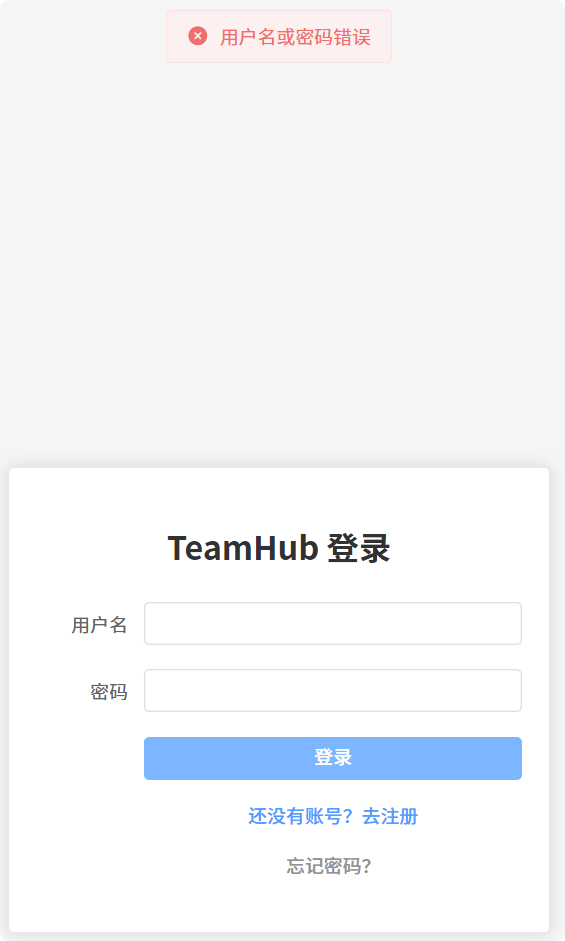
\includegraphics[width=\textwidth]{截图/dl1.png}\end{minipage}
\begin{minipage}{0.4\textwidth}\centering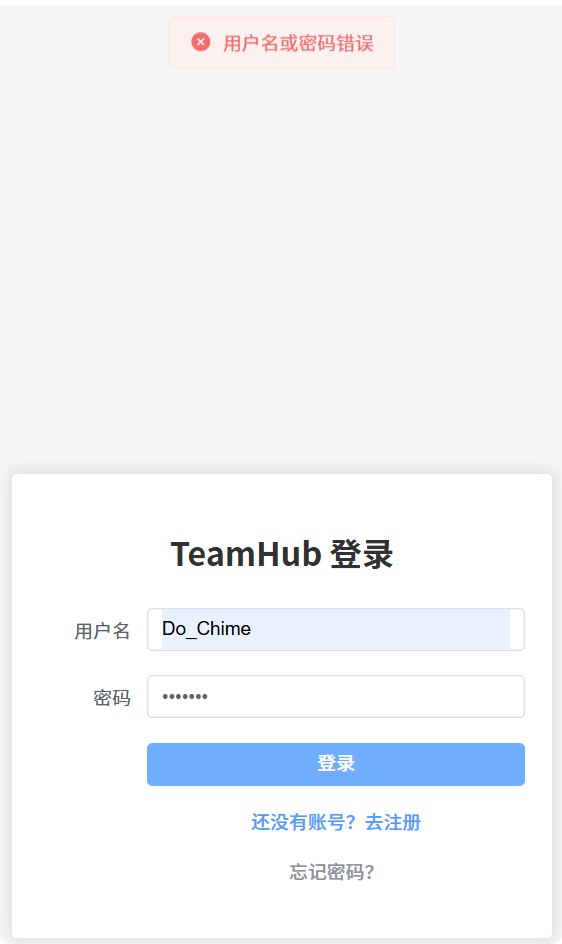
\includegraphics[width=\textwidth]{截图/dl2.png}\end{minipage}


\includegraphics[width=14cm]{截图/dl3.png}
\caption{登录功能测试截图}
\end{figure}
% 【图片位置】贴上登录测试三个用例的运行截图

\textbf{注册功能。}测试用户注册功能。队长注册时需填写球队名称，系统自动生成邀请码；队员注册时需填写邀请码加入已有球队。测试结果如表\ref{tab:test-register}所示。

\begin{table}[H]
\centering
\caption{注册功能测试用例表}
\label{tab:test-register}
\begin{tabular}{p{4.5cm}p{4.5cm}p{5.5cm}}
\toprule
\textbf{用例1} & \textbf{用例2} & \textbf{用例3}\\
\midrule
队长注册：填写用户名、密码、姓名、入学年份、球队名称，信息合法。 & 队员注册：填写用户名、密码、姓名、入学年份、正确的邀请码。 & 队员注册：填写用户名、密码、姓名、入学年份、过期的邀请码。\\
\midrule
注册成功，返回role=CAPTAIN和inviteCode，可登录。 & 注册成功，返回role=MEMBER和teamName，可登录。 & 返回400，提示"邀请码无效或已过期"。\\
\bottomrule
\end{tabular}
\end{table}

% 第一行左右并列
\begin{center}
\begin{minipage}{0.4\textwidth}\centering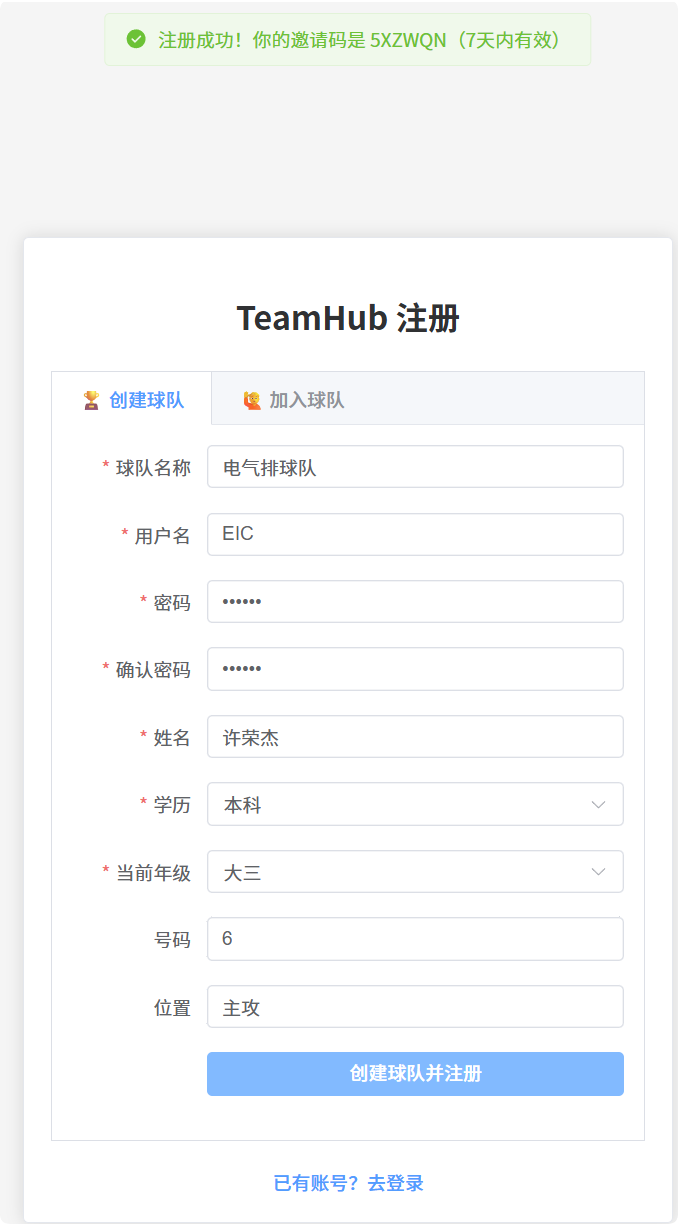
\includegraphics[width=\textwidth]{截图/zc0.png}\end{minipage}
\hspace{0.4cm}
\begin{minipage}{0.4\textwidth}\centering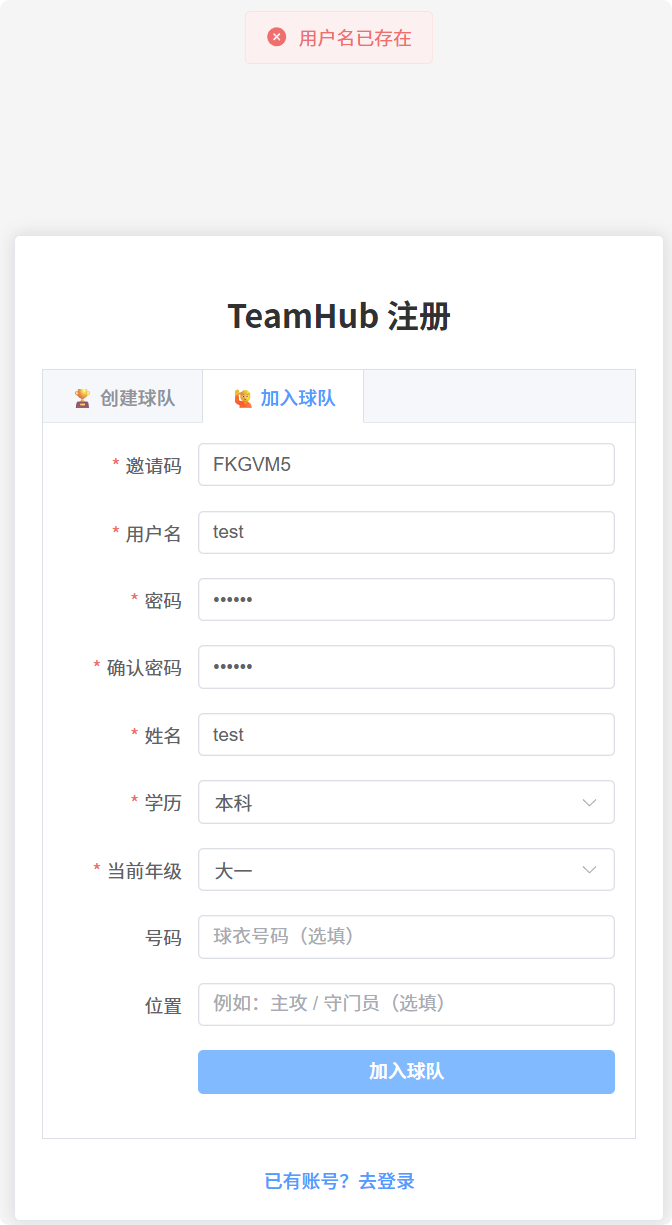
\includegraphics[width=\textwidth]{截图/zc1.png}\end{minipage}
\end{center}

\vspace{0.2cm}

% 第二行左右并列
\begin{center}
\begin{minipage}{0.4\textwidth}\centering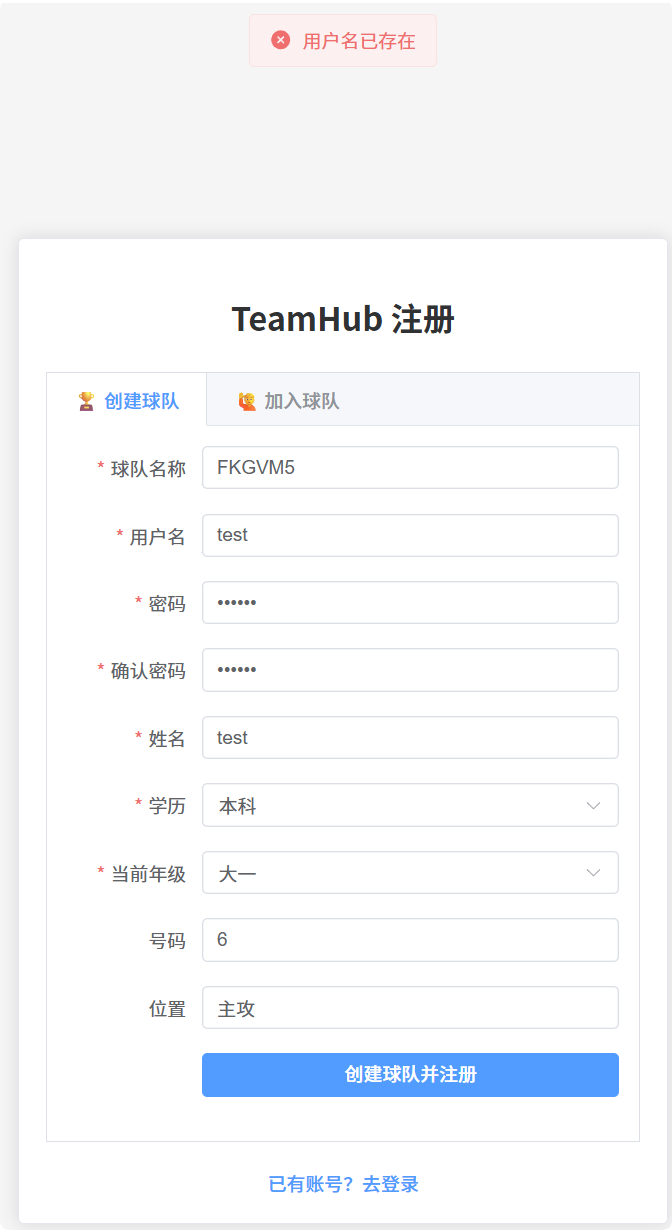
\includegraphics[width=\textwidth]{截图/zc2.png}\end{minipage}
\hspace{0.4cm}
\begin{minipage}{0.4\textwidth}\centering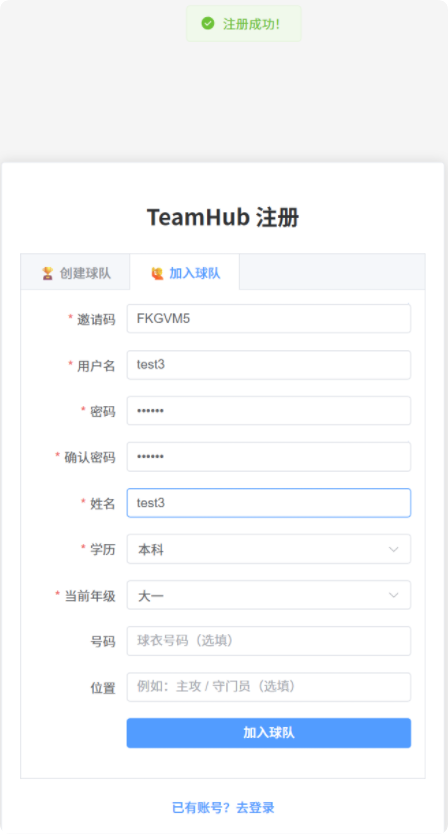
\includegraphics[width=\textwidth]{截图/zc3.png}\end{minipage}
\end{center}
\captionof{figure}{注册功能测试截图}

% 【图片位置】贴上注册测试三个用例的运行截图

\textbf{训练报名功能。}测试训练报名功能，首先要判断训练是否已结束（trainTime+3小时），其次要判断报名动作是新增还是修改已有记录。测试结果如表\ref{tab:test-training}所示。

\begin{table}[H]
\centering
\caption{训练报名功能测试用例表}
\label{tab:test-training}
\begin{tabular}{p{5cm}p{5cm}p{4.5cm}}
\toprule
\textbf{用例1} & \textbf{用例2} & \textbf{用例3}\\
\midrule
队员对一场未结束的训练点击"参加"。此前该队员无报名记录。 & 队员对一场已报名的训练修改状态为"请假"，并填写原因。 & 队员对一场已结束的训练（trainTime+3h已过）尝试修改报名状态。\\
\midrule
signup表新增一条status=ATTEND的记录。 & signup表同一条记录的status更新为ABSENT，reason有值。 & 返回400，提示"训练已结束，无法修改报名状态"。\\
\bottomrule
\end{tabular}
\end{table}

% ========== 训练报名（1张图） ==========
\begin{figure}[H]
\centering
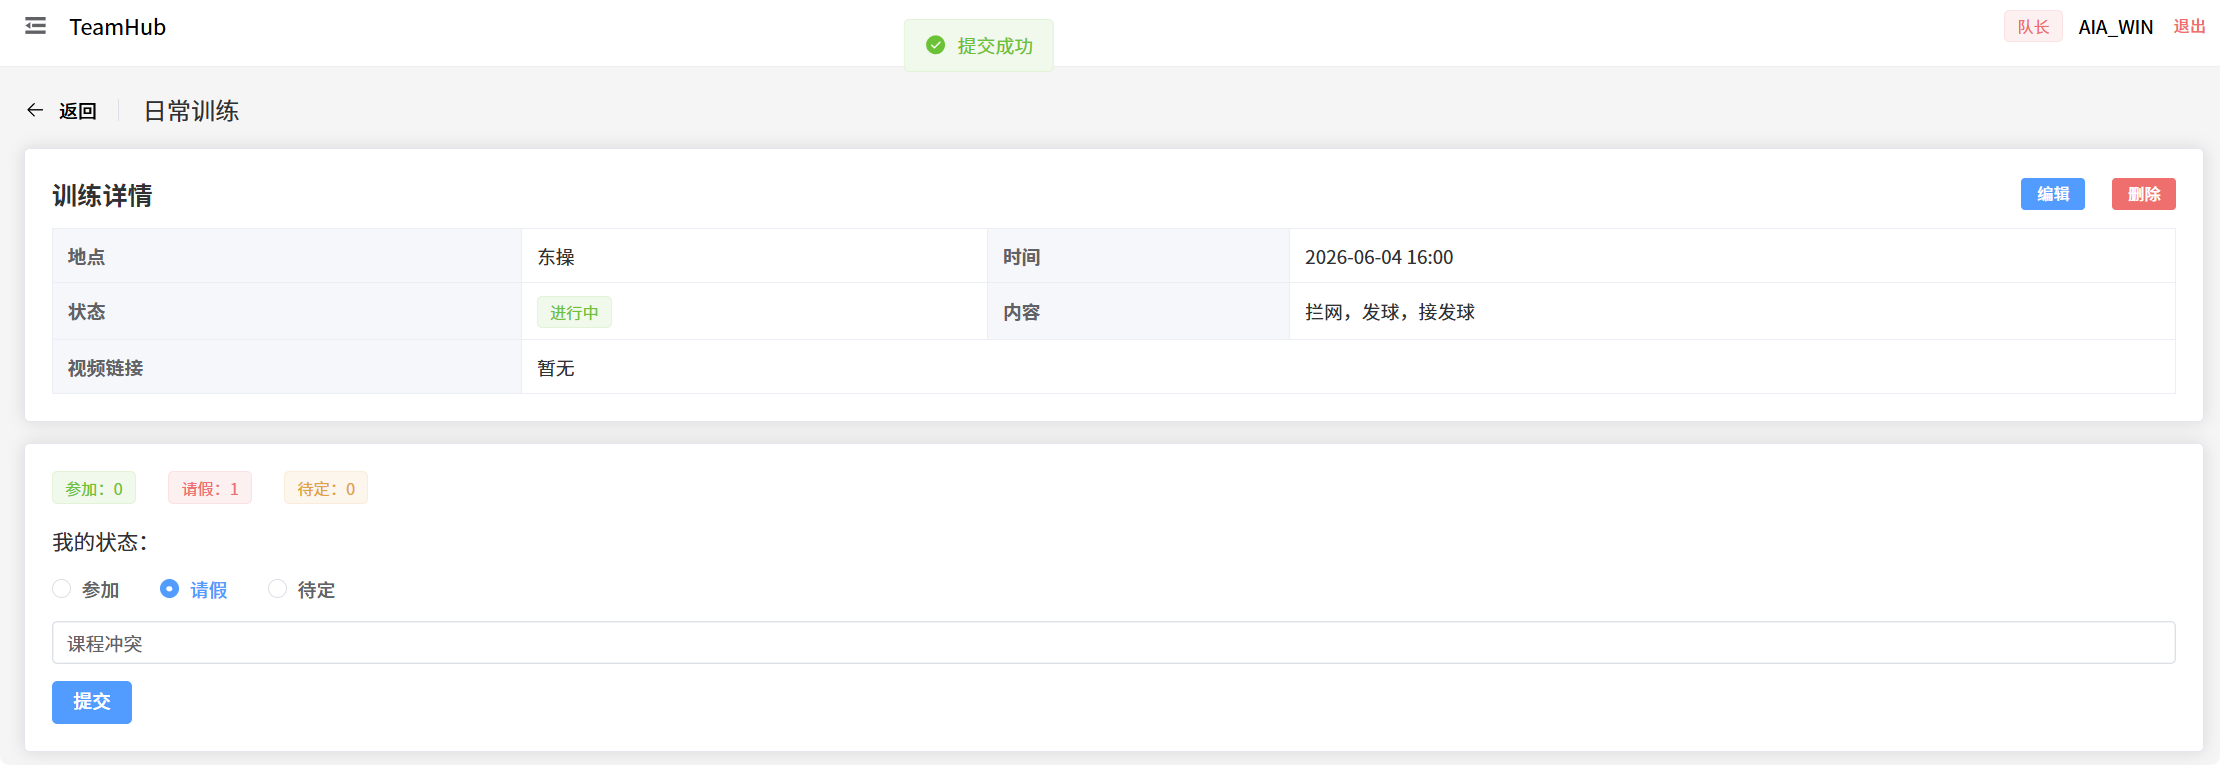
\includegraphics[width=0.85\textwidth]{截图/xl1.png}
\caption{训练报名功能测试截图}
\end{figure}
% 【图片位置】贴上训练报名测试截图（展示训练详情页及报名状态）

\textbf{比赛比分编辑功能。}测试比赛的多小局比分编辑，采用"先删后插"策略。测试结果如表\ref{tab:test-match}所示。

\begin{table}[H]
\centering
\caption{比赛比分编辑功能测试用例表}
\label{tab:test-match}
\begin{tabular}{p{4.5cm}p{4.5cm}p{5.5cm}}
\toprule
\textbf{用例1} & \textbf{用例2} & \textbf{用例3}\\
\midrule
创建一场排球训练赛，录入3局比分（25:20, 23:25, 15:10）。 & 编辑已有比赛的比分，将3局改为5局。 & 将比赛状态标记为FINISHED后尝试再次修改比分。\\
\midrule
match\_set表新增3条记录，set\_number分别为1/2/3。 & match\_set表中旧3条被删除，新5条被insert，set\_number从1到5递增。 & 可以修改（比分更新的updateSets不检查状态，仅updateStatus检查）。\\
\bottomrule
\end{tabular}
\end{table}

% ========== 比赛比分（1张图） ==========
\begin{figure}[H]
\centering
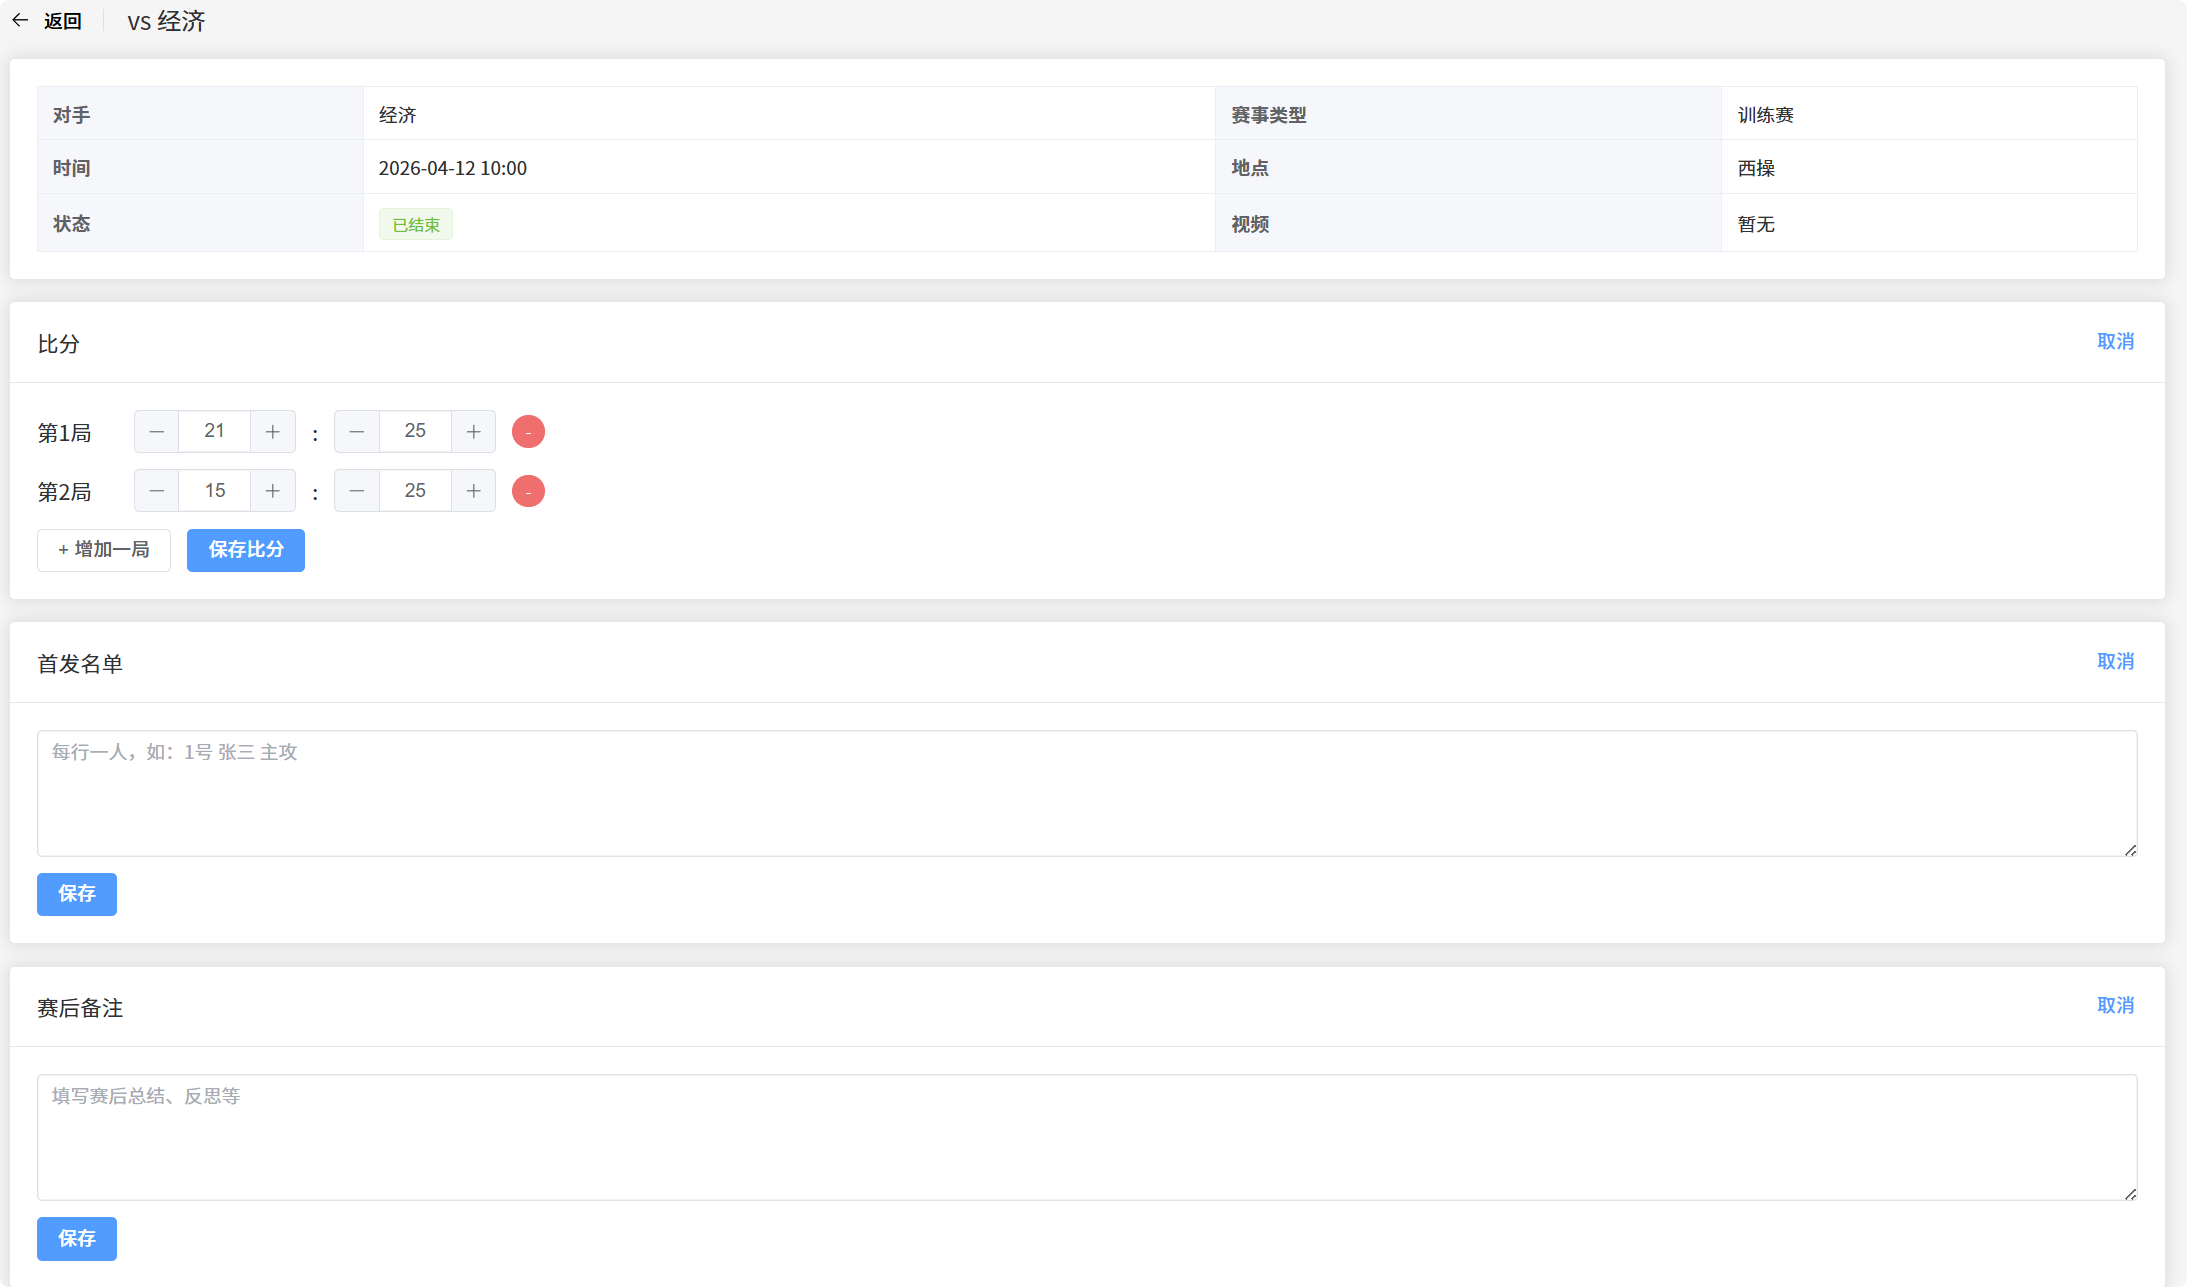
\includegraphics[width=0.85\textwidth]{截图/bs1.png}
\caption{比赛比分编辑功能测试截图}
\end{figure}
% 【图片位置】贴上比赛比分编辑测试截图（展示比赛详情及比分）

\textbf{权限控制功能。}测试CAPTAIN和MEMBER两类角色对敏感操作的权限差异。测试结果如表\ref{tab:test-perm}所示。

\begin{table}[H]
\centering
\caption{权限控制测试用例表}
\label{tab:test-perm}
\begin{tabular}{p{4.5cm}p{4.5cm}p{5.5cm}}
\toprule
\textbf{用例1} & \textbf{用例2} & \textbf{用例3}\\
\midrule
MEMBER调用POST /api/training/create（发布训练，标注@PreAuthorize("hasRole('CAPTAIN')")）。 & CAPTAIN调用POST /api/training/create。 & MEMBER尝试编辑另一位球员的资料（PUT /api/player/:id）。\\
\midrule
返回403，通过Spring Security的AccessDeniedException拦截，ElMessage提示"无权操作"。 & 返回200，训练创建成功，并自动在时光轴记录autoTrainingCreated事件。 & 返回400，PlayerController.update()中判断既非队长也非本人，抛RuntimeException"无权编辑他人资料"。\\
\bottomrule
\end{tabular}
\end{table}

\textbf{发展中心点赞功能。}测试建议点赞的toggle机制。测试结果如表\ref{tab:test-like}所示。

\begin{table}[H]
\centering
\caption{点赞功能测试用例表}
\label{tab:test-like}
\begin{tabular}{p{4.5cm}p{4.5cm}p{5.5cm}}
\toprule
\textbf{用例1} & \textbf{用例2} & \textbf{用例3}\\
\midrule
用户对某条未点赞的个人建议点击点赞按钮。 & 用户对已点赞的同一条建议再次点击。 & 用户对球队建议执行同样的点赞/取消操作。\\
\midrule
player\_suggestion\_like表新增记录，likes字段+1，前端按钮变蓝。 & player\_suggestion\_like表该记录被deleteById，likes字段-1（Math.max(0, likes-1)），前端按钮恢复灰色。 & 逻辑完全相同，操作表切换为team\_suggestion\_like和team\_suggestion。\\
\bottomrule
\end{tabular}
\end{table}

\begin{figure}[H]
\centering
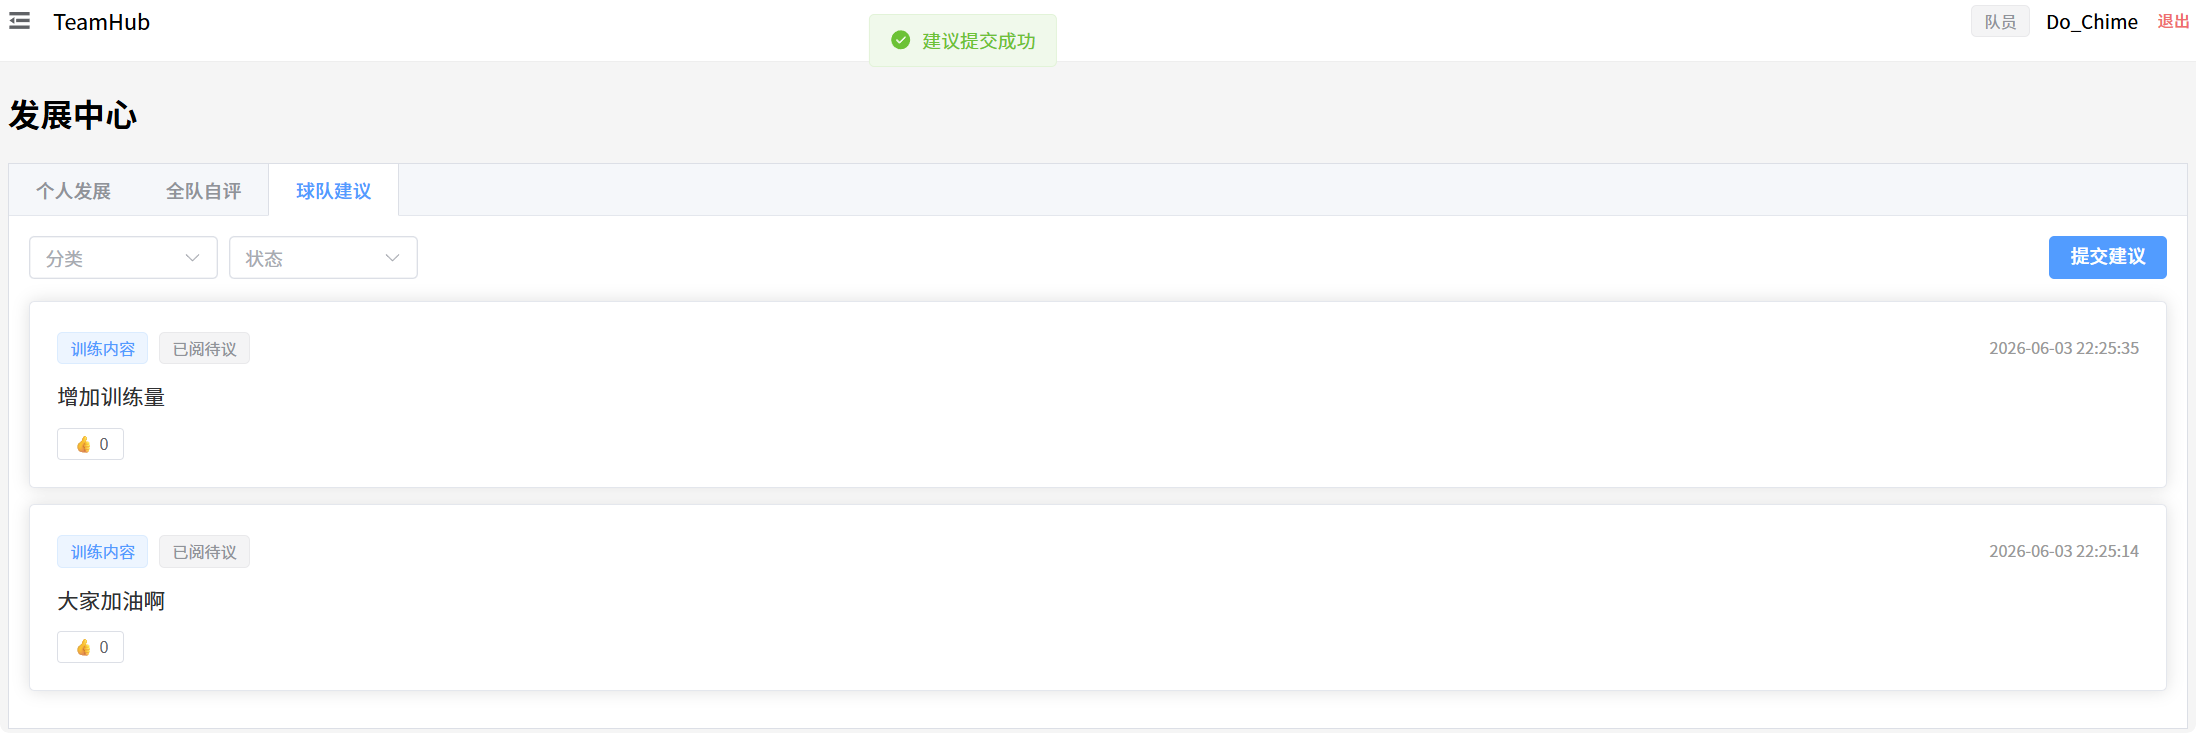
\includegraphics[width=0.85\textwidth]{截图/jy1.png}

\vspace{0.4cm}

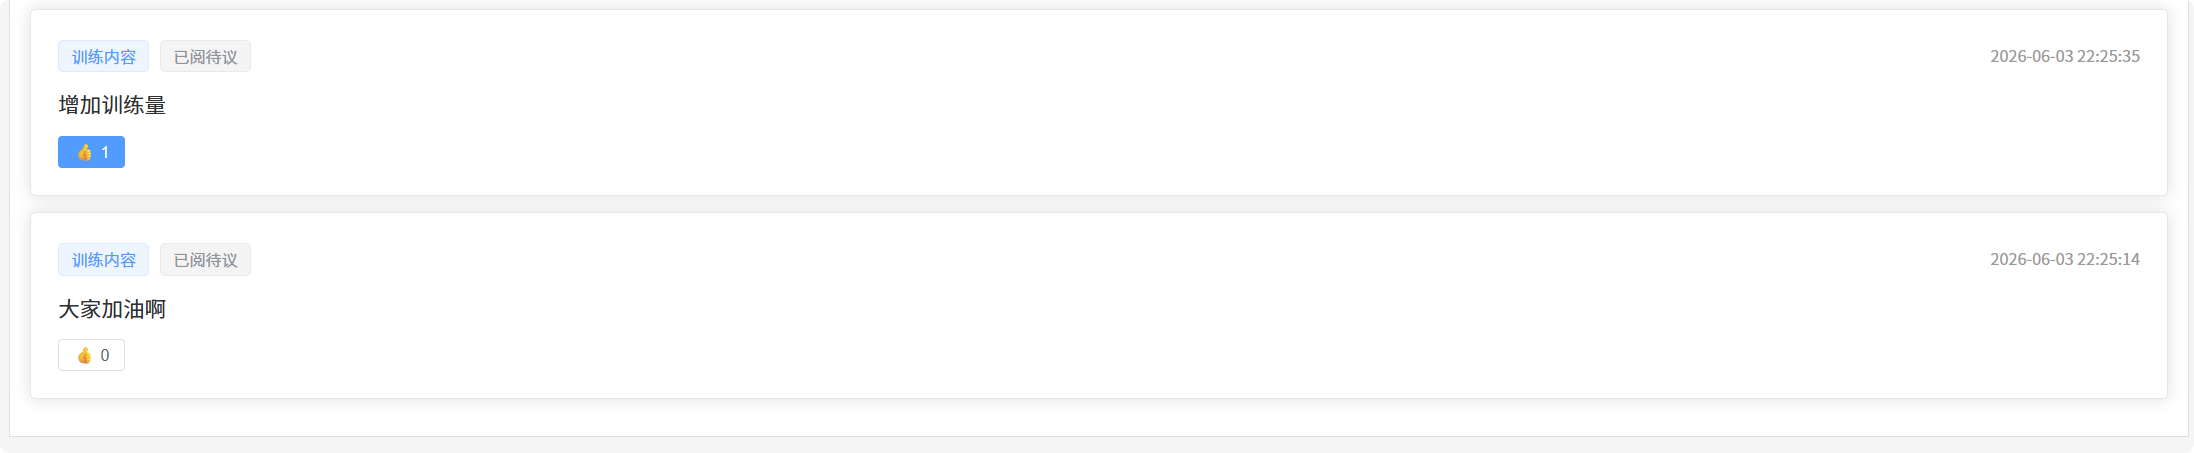
\includegraphics[width=0.85\textwidth]{截图/dz1.png}
\caption{点赞功能测试截图}
\end{figure}

% 【图片位置】贴上点赞测试截图

\textbf{毕业迁移功能。}测试队长将球员从当打之年（ACTIVE）迁移至功勋人物（ALUMNI）的权限与数据一致性。测试结果如表\ref{tab:test-graduate}所示。

\begin{table}[H]
\centering
\caption{毕业迁移功能测试用例表}
\label{tab:test-graduate}
\begin{tabular}{p{4.5cm}p{4.5cm}p{5.5cm}}
\toprule
\textbf{用例1} & \textbf{用例2} & \textbf{用例3}\\
\midrule
队长对一位ACTIVE状态的球员点击"毕业迁移"。 & 队长对一位已经是ALUMNI状态的球员再次点击"毕业迁移"。 & MEMBER尝试调用PUT /api/player/:id/graduate。\\
\midrule
player表该记录status变为ALUMNI，timeline\_event表自动插入一条AUTO类型的退役事件。 & 状态已是ALUMNI，重复迁移无实际数据变化（updateById幂等）。 & 返回403，Spring Security的@PreAuthorize拦截，提示"无权操作"。\\
\bottomrule
\end{tabular}
\end{table}


\textbf{时光轴功能。}测试人工事件的发布、编辑权限及自动事件生成。测试结果如表\ref{tab:test-timeline}所示。

\begin{table}[H]
\centering
\caption{时光轴功能测试用例表}
\label{tab:test-timeline}
\begin{tabular}{p{4.5cm}p{4.5cm}p{5.5cm}}
\toprule
\textbf{用例1} & \textbf{用例2} & \textbf{用例3}\\
\midrule
队长发布一条人工事件，选择关联类型为"训练"并填写trainingId。 & 事件的原始作者（MEMBER）修改自己发布的人工事件的标题和描述。 & MEMBER尝试编辑另一位队员发布的人工事件。\\
\midrule
timeline\_event表新增一条MANUAL记录，ref\_training\_id有值，事件在时间轴正确展示。 & 调用PUT /api/timeline/:id成功，事件内容更新，eventTime不变。 & 返回400，后端校验当前用户既不是作者也不是队长，抛RuntimeException"无权编辑"。\\
\bottomrule
\end{tabular}
\end{table}

% ========== 时光轴（1张图） ==========
\begin{figure}[H]
\centering
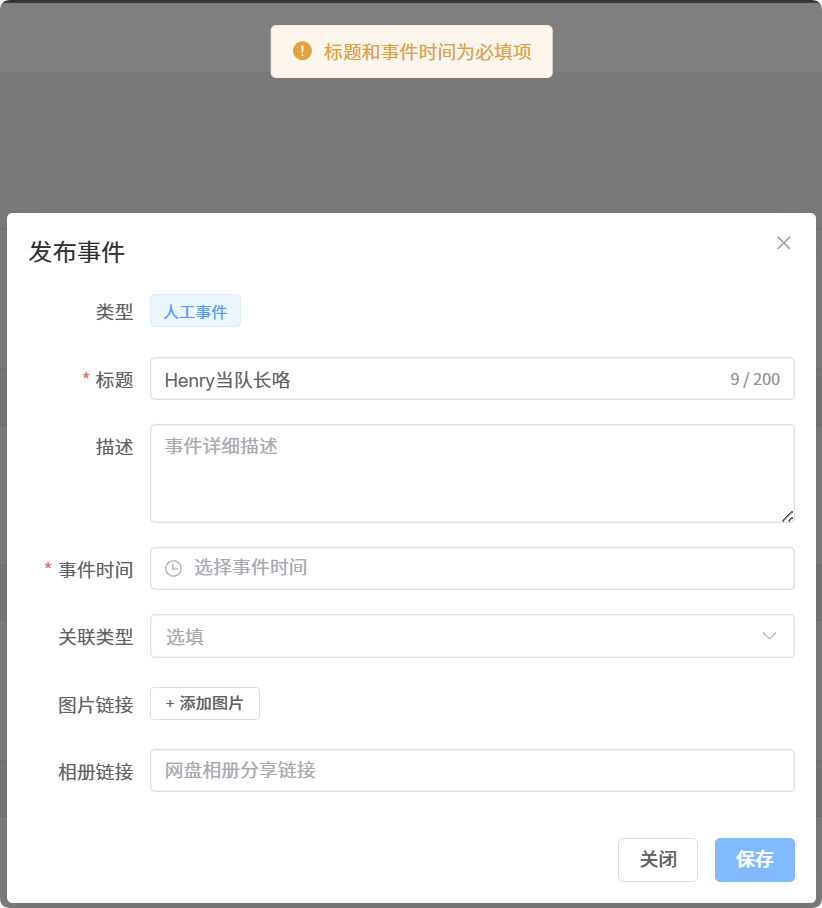
\includegraphics[width=0.85\textwidth]{截图/sgz1.png}
\caption{时光轴功能测试截图}
\end{figure}
% 【图片位置】贴上时光轴测试截图


\subsection{结果分析}

系统可以正确实现登录功能。当用户输入的用户名或密码为空或不匹配时，系统都能正确通知用户错误信息；当用户输入正确时，也能正确跳转至首页仪表盘。

系统可以正确实现注册功能。队长注册时自动生成6位邀请码，队员注册时校验邀请码有效性（检查invite\_code\_expires\_at是否晚于当前时间）。邀请码过期或无效时正确报错。

系统可以正确实现训练发布、接龙报名、报名统计功能。训练发布后时光轴自动产生AUTO事件。报名时正确判断训练是否已结束（trainTime+3小时截止机制）。报名列表实时显示各状态人数。出勤率按"已参加次数/总训练次数"计算，结果保留一位小数。

系统可以正确实现比赛的创建、多小局比分编辑、状态流转功能。比分的"先删后插"策略在多次修改后数据保持一致（无冗余记录，set\_number递增正确）。比赛一旦标记FINISHED则状态不可回退。

系统可以正确实现球员档案的双标签页展示和年级自动推算。年级计算算法在本科/硕士/博士三种学位、不同入学年份和跨月份（9月开学季前后）的组合下均输出正确结果（如2024级本科在2025年3月显示"大一"，2025年9月显示"大二"）。毕业迁移功能触发后球员从ACTIVE变为ALUMNI并写入时光轴退役事件，历史数据完整保留。

系统可以正确实现发展中心的自评、互评建议、球队建议功能。点赞toggle机制在点赞和取消之间正确切换，likes字段通过Math.max(0, likes-1)防止出现负数。被举报建议正确进入队长审核列表。

系统可以正确实现时光轴的按年份/月份筛选和自动/人工事件展示。自动事件不可编辑，人工事件仅作者和队长可编辑。年份筛选通过SQL的YEAR()和MONTH()函数实现。

系统可以正确实现球队设置的邀请码管理、队长传承、成员管理功能。队长传承后老队长角色自动降级为MEMBER，新队长升级为CAPTAIN，双方Token失效需重新登录。

\textbf{已知问题与改进方向。}测试过程中发现以下可改进点：
\begin{enumerate}[label=(\arabic*)]
\item \textbf{分页加载}：训练列表、比赛列表、时光轴目前为一次性全量加载，数据量增大时可能影响性能，后续应接入MyBatis-Plus分页和el-pagination；
\item \textbf{出勤率学期分段}：当前出勤率统计全部历史训练（不分学期），导致新学期初出勤率偏低，后续应按学年/学期分段计算；
\item \textbf{图床集成}：图片字段依赖用户手动粘贴外部URL，门槛较高，后续可集成SM.MS等免费图床API实现一键上传；
\item \textbf{时光轴精准跳转}：点击关联的训练/比赛链接目前仅跳转到列表页，未携带具体ID，后续应改为带参数的路由跳转。
\end{enumerate}


% ==============================
%  第5章 用户反馈和结论
% ==============================
\newpage
\section{用户反馈和结论}

\subsection{用户反馈}

在系统上线并运行一段时间后，为了改进系统功能、提升用户体验，我们向球队成员收集了用户反馈。根据反馈结果，总体来说用户对系统功能满意度较高，认为系统便捷、实用、好用。

\textbf{使用场景。}队长日常在系统内发布训练和比赛通知，队员通过手机或电脑登录系统查看详情并接龙报名。比赛结束后，队长及时录入比分、上传视频链接并更新比赛状态为FINISHED。发展中心的自评和互评功能在每周训练总结会上由队员填写，球队建议板块用于收集队员对整体训练安排的意见。

\textbf{具体反馈摘录如下：}
\begin{enumerate}[label=(\arabic*)]
\item \textbf{训练报名管理}："系统自动算出勤率很方便，不需要人工统计Excel了，之前每次比赛前都要手动数哪些人来了，现在看仪表盘一眼就能看到。"
\item \textbf{年级自动推算}："之前维护年级表格很头疼，每年9月都要全员更新，现在系统自己算，大一到大四、研一到研三都能自动出来，还能看到已经毕业的学长学姐。"
\item \textbf{多局比分记录}："排球比赛打满5局很常见，以前用共享文档每次都要手写比分，现在可以直接在线录入，比分的增删改很灵活。"
\item \textbf{时光轴}："球队的历史可视化做的不错，特别是新队员入队时能看到前辈的成长轨迹，很有归属感。自动事件很方便，不需要手动记录每一次训练和比赛。"
\item \textbf{发展中心}："匿名建议这个功能挺好的，有些意见当面不太好说，通过匿名可以传达出来。点赞和采纳状态也能看出大家普遍关注什么问题。"
\end{enumerate}

\subsection{测试结论}

在单元测试和集成测试的基础上，我们对系统进行系统测试。对于用户多次输入同样的测试用例，系统始终返回一致的结果，响应时间在可接受范围内（绝大多数接口小于100ms，复杂聚合接口如首页仪表盘小于300ms）。

经过全面的功能测试与性能验证，TeamHub高校球队数字化档案管理系统各项功能运行稳定，在交互体验、数据管理、权限控制等方面均达到了预期设计目标。系统能够有效支撑高校球队日常训练安排、比赛记录、人员管理和成长追踪等核心业务场景，为球队的信息化管理提供了有力支持。

\subsection{总结}

本项目为高校球队开发了一款数字化档案管理系统，采用前后端分离架构，实现了训练中心、比赛中心、球员档案、发展中心、时光轴、球队设置、管理后台七大功能模块。

\textbf{队友A}负责后端开发，完成了Spring Boot项目骨架搭建、13张数据库表设计、全部8个Controller/Service/Mapper实现、JWT认证、全局异常处理、Spring Security权限配置以及Linux云服务器部署。队友A设计的后端架构清晰分层，复用性高，为前端开发提供了稳定的REST API支撑。

\textbf{队友B}负责前端开发与完善工作，实现了全部页面组件开发、Vue Router路由与导航守卫、Axios请求/响应拦截器封装、响应式布局适配、ECharts图表绘制以及前后端联调。队友B在开发与完善过程中发现并及时修复了若干边界情况（如训练截止时间的毫秒级精度问题），对提升系统健壮性起到了关键作用。

项目开发过程中，两名组员分工明确、协作高效：每周进行线下同步会议，使用GitHub Issues记录待办事项和Bug追踪，采用Git分支管理进行功能开发。项目从需求分析到最终部署共历时约5周，所有核心功能均按时交付并通过测试。

系统的不足之处包括：未实现图床集成导致图片上传门槛高，未实现出勤率按学期分段统计，时光轴跳转缺少精准定位，部分长列表未做分页。这些改进方向已列入后续开发计划。



% ==============================
%  第6章 总结和体会
% ==============================
\newpage
\section{总结和体会}

\subsection{队友A的总结}

在本次软件工程课程中，我与队友B合作完成了院队数字档案系统TeamHub。我主要负责后端开发，包括数据库设计、Spring Boot项目搭建、JWT认证配置、RESTful API实现以及Linux服务器部署运维。走完整套流程后，我对软件工程的理解比单纯的写代码深了不少。

\textbf{需求分析决定方向。}以前觉得写代码才是核心，这次发现需求分析阶段的投入直接决定了后面的工作是否跑偏。例如发展中心模块，最初只考虑球员自评，后来和队友深入沟通后才补上队友互评建议和球队建议两个维度——前者解决人的问题，后者解决事的问题。如果前期不花时间理解真实场景，后面的代码写得再快也是偏离目标的。

\textbf{技术选型要务实。}技术选型时我砍掉了Redis和Docker，不是因为它们不好，而是对于这个规模的项目属于过度设计。在pom.xml里处理MyBatis-Plus 3.5.12与mybatis-spring 3.0.4的版本冲突时，我切实体会到"引入依赖容易，解决冲突才是难"。JWT认证链路的完整实现让我对安全机制有了体系化认知：Token生成→前端携带→Filter解析→SecurityContext注入→@PreAuthorize鉴权→全局异常处理，每个环节都不能缺。

\textbf{数据库设计比代码更能保证一致性。}发展中心的点赞功能最初想在player\_suggestion表里加个布尔字段标记是否点赞，后来发现并发点击会导致likes计数错乱。改成独立的player\_suggestion\_like表，用(user\_id, suggestion\_id)联合唯一约束，点赞和取消就变成了可靠的原子操作。这个经历让我意识到，很多看似代码层面的问题，根源在表结构设计阶段就已经注定了。

\textbf{部署是开发的最后一公里。}本地跑通和部署上线完全是两回事。Nginx反向代理配置、systemd服务守护、跨域白名单、服务器防火墙放行8080端口——这些细节任何一处没配好，前端请求都会404或403。印象最深的一次是jar包上传后重启服务正常，但前端访问/api报错，排查了半小时才发现是Nginx的proxy\_pass末尾多了个斜杠导致路径拼接错误。这类问题不会被单元测试捕获，只有在真实部署环境中才会暴露。

\textbf{团队协作与时间分配。}我和队友B采用前后端分离的分工，每周线下同步一次进度，用GitHub Issues记录待办事项。前期我进展较快，第1-2周就完成了JWT和数据库建表。但后期临近考试周，接口文档和测试用例的整理被压缩到很短时间，好在前期代码注释足够，最后只是把已有的素材组织成章节。下次应该边开发边产出文档，而不是攒到最后。

从敲第一行建表SQL到最终在Nginx上部署成功，这条路走完之后，再看任何一个Web系统的架构图都不会觉得陌生。数据库里一条entry\_year如何在Vue页面上变成"大三"，JWT中的role字段如何在@PreAuthorize里拦下越权请求——这种数据从后端流到前端再流回来的全景认知，是这次项目给我最大的收获。

\subsection{队友B的总结}

在本次项目中，我主要负责前端开发与完善工作，同时承担了服务器部署和运维的任务。从Vue项目初始化到最终把系统跑在云服务器上，这段经历让我对"前端不只是写页面"有了切身体会。

\textbf{前端架构与组件化思维。}项目一开始我是从零搭建Vue 3 + Vite骨架的，路由守卫、Axios拦截器封装、Layout响应式布局这些基础设施花了不少时间。特别是Layout.vue的桌面端侧边栏和移动端抽屉切换，通过window.innerWidth < 768判断，配合el-aside和el-drawer两套UI，让我理解了响应式不只是CSS媒体查询，还包括交互模式的切换。Element Plus的组件确实提高了效率，但深度定制时也会踩坑——比如el-date-picker的时区问题，JS Date对象经Axios JSON.stringify后调用toISOString()变成UTC时间，导致后端存储少8小时。最后改成手动格式化为本地时间字符串才解决。这类Bug和业务逻辑无关，但会直接影响用户体验。

\textbf{前后端联调是双向沟通。}联调阶段我最大的感受是：接口文档再详细，也替代不了面对面沟通。例如训练报名接口最初只返回字符串"报名成功"，但我前端需要刷新报名状态标签，于是又和队友A商量改成返回更新后的signup对象。还有比赛比分的"先删后插"策略，前端不需要区分增删改，只需把当前整组比分POST过去，这个设计减少了双方很多不必要的麻烦。好的API设计应该是让调用方感到舒服，而不是让实现方感到方便。

\textbf{部署是另一门课。}服务器部署之前我以为就是"上传jar包、运行、完事"，实际操作时发现Nginx配置、systemd服务守护、防火墙放行、静态资源路径，任何一处出错都会导致服务不可用。最离谱的一次是前端dist上传后页面白屏，排查半天发现是Nginx的try\_files没配好，直接访问路由时返回了404而不是index.html。这些经验让我明白，DevOps不是后端专属，前端开发者也应该了解部署链路，否则出了问题连排查方向都不知道。

\textbf{迭代开发比一步到位更现实。}项目初期我想把所有页面都设计得很完美再开始写代码，结果两周过去了还在调配色。后来改为按模块逐个交付：先让训练中心能完整跑通（列表→详情→报名），再复制模式到比赛中心、球员档案等模块。每个模块端到端可用后再做细节优化。这种增量式开发让我每周都有可见的产出，也便于及时根据队友A的接口调整前端逻辑。

这次项目让我真正理解了全栈视角的价值：写前端时知道后端的数据是怎么来的，部署时知道请求是怎么被Nginx转发的。以前看别人的系统总觉得 magically works，现在再看任何一个Web应用，脑子里会自然浮现出请求从前端出发，经过Nginx、Tomcat、Service、Mapper，最后落到数据库里那一整条链路。这种通透感，是课本和教程给不了的。

% ==============================
%  附录
% ==============================
\newpage
\section*{附录}
\addcontentsline{toc}{section}{附录}

\subsection*{A.1 \quad API接口清单}

以下是系统核心RESTful API接口概览。

\textbf{用户认证（/api/user）}
\begin{itemize}[leftmargin=2em]
\item POST /api/user/register — 注册（队长注册含teamName字段，队员注册含inviteCode）
\item POST /api/user/login — 登录（返回JWT Token + 用户信息）
\item GET /api/user/me — 获取当前登录用户信息
\end{itemize}

\textbf{训练管理（/api/training）}
\begin{itemize}[leftmargin=2em]
\item GET /api/training — 训练列表（含isFinished虚拟字段）
\item POST /api/training/create — 创建训练（仅队长）
\item PUT /api/training/:id — 编辑训练（仅队长）
\item DELETE /api/training/:id — 删除训练及关联报名记录（仅队长）
\item POST /api/training/:id/signup — 报名（ATTEND/ABSENT/PENDING）
\item GET /api/training/:id/signups — 报名统计列表
\end{itemize}

\textbf{比赛管理（/api/match）}
\begin{itemize}[leftmargin=2em]
\item GET /api/match — 比赛列表（支持gameType筛选）
\item POST /api/match/create — 创建比赛（仅队长）
\item PUT /api/match/:id/sets — 更新比分（先删后插策略）
\item PUT /api/match/:id/status — 更新比赛状态
\end{itemize}

\textbf{球员管理（/api/player）}
\begin{itemize}[leftmargin=2em]
\item GET /api/player — 球员列表（ACTIVE/ALUMNI双标签）
\item GET /api/player/:id — 球员详情（含role注入）
\item PUT /api/player/:id — 编辑球员（权限差异控制）
\item PUT /api/player/:id/graduate — 毕业迁移（仅队长）
\end{itemize}

\textbf{发展中心（/api/development）}
\begin{itemize}[leftmargin=2em]
\item POST /api/development/self-review — 提交自评
\item GET /api/development/player-suggestion — 个人建议列表（含likedByMe注入）
\item POST /api/development/player-suggestion/:id/like — 点赞toggle
\item POST /api/development/player-suggestion/:id/report — 举报建议
\item GET /api/development/team-suggestion — 球队建议列表
\item POST /api/development/team-suggestion/:id/like — 球队建议点赞
\item POST /api/development/team-suggestion/:id/response — 队长回应
\end{itemize}

\textbf{时光轴（/api/timeline）}
\begin{itemize}[leftmargin=2em]
\item GET /api/timeline — 事件列表（支持year/month筛选）
\item POST /api/timeline — 发布人工事件（必须关联训练/比赛/球员之一）
\item PUT /api/timeline/:id — 编辑人工事件（仅作者和队长）
\end{itemize}

\textbf{球队设置（/api/team）}
\begin{itemize}[leftmargin=2em]
\item GET /api/team — 获取球队信息和邀请码
\item POST /api/team/refresh-invite-code — 重新生成邀请码
\item PUT /api/team/name — 修改队名
\item PUT /api/team/captain/:userId — 队长传承
\item DELETE /api/team/member/:userId — 删除成员
\item DELETE /api/team — 解散球队（级联删除）
\end{itemize}

\textbf{管理后台（/api/admin）}
\begin{itemize}[leftmargin=2em]
\item GET /api/admin/reported-suggestions — 被举报建议列表
\item POST /api/admin/reported-suggestions/:id/ignore — 忽略举报
\item DELETE /api/admin/reported-suggestions/:id — 删除建议
\end{itemize}

\textbf{仪表盘（/api/dashboard）}
\begin{itemize}[leftmargin=2em]
\item GET /api/dashboard — 首页聚合数据（upcomingTrainings/recentMatches/attendance/pendingSuggestions等）
\end{itemize}

\subsection*{A.2 \quad 数据库表结构}

系统共包含13张业务表，表名及其简要说明如下：

\begin{table}[H]
\centering
\caption{数据库表清单}
\begin{tabular}{p{4.5cm}p{9cm}}
\toprule
\textbf{表名} & \textbf{说明} \\
\midrule
user & 用户登录信息（密码BCrypt存储，角色MEMBER/CAPTAIN） \\
player & 球员档案（entryYear是年级计算的唯一输入） \\
team & 球队信息（邀请码6位，7天有效期） \\
training & 训练安排（trainTime+3小时为截止判断依据） \\
training\_signup & 训练报名表（联合唯一约束uk\_training\_user） \\
match\_game & 比赛信息（status控制可编辑性） \\
match\_set & 比赛比分（每场比赛1~N条，先删后插策略） \\
player\_self\_review & 球员自评（currentProblem/improvementGoal必填） \\
player\_suggestion & 个人建议（含举报字段isReported） \\
player\_suggestion\_like & 个人建议点赞（联合唯一约束） \\
team\_suggestion & 球队建议（含队长回应字段） \\
team\_suggestion\_like & 球队建议点赞 \\
timeline\_event & 时光轴事件（AUTO/MANUAL，必须关联训练/比赛/球员之一） \\
\bottomrule
\end{tabular}
\end{table}

\end{document}
